\documentclass[12pt]{article}
 
\usepackage[margin=1in]{geometry} 
\usepackage{amsmath,amsthm,amssymb,float,graphicx,mathtools,tikz,hyperref}
\usepackage[at]{easylist}
\usepackage{indentfirst}
\usepackage{ragged2e}
\RaggedRightParindent = 24 pt
\setlength{\parskip}{1.5em}
\renewcommand{\baselinestretch}{1.5}
\usepackage{algorithm2e}
\usepackage{graphicx}
\usepackage{titling}
\renewcommand\maketitlehooka{\null\mbox{}\vfill}
\renewcommand\maketitlehookd{\vfill\null}
\usepackage{tocloft}
\renewcommand\cftsecafterpnum{\vskip6pt}

\usepackage{mdframed}
\usetikzlibrary{patterns,hobby}
\usepackage{tcolorbox}
\newtcolorbox{mybox}{colback=red!5!white,colframe=red!75!black,fonttitle=\bfseries,title=Box}
\newtcolorbox{imp}{colback=orange!5!white,colframe=orange!75!white}
\newcommand{\redp}[1]{\textcolor{red}{#1}}
\newcommand{\bluep}[1]{\textcolor{blue}{#1}}
    
\usepackage{xcolor}
\usepackage{listings}
\lstset{basicstyle=\ttfamily,
  showstringspaces=false,
  commentstyle=\color{red},
  keywordstyle=\color{blue}
}
\usepackage{stackengine}
\renewcommand{\theequation}{\thesection.\arabic{equation}}
\renewcommand{\thefigure}{\thesection.\arabic{figure}}
\renewcommand{\arraystretch}{0.01}

\usepackage{chngcntr}
\counterwithin{table}{section}
\counterwithin{equation}{section}
\counterwithin{figure}{section}

\usepackage{circledsteps}
\def\selfcirc{
\tikz[x=0.5pt,y=0.5pt,yscale=-1,xscale=1,baseline=-8.0ex]{
\draw   (81,85.6) .. controls (81,75.33) and (89.33,67) .. (99.6,67) .. controls (109.87,67) and (118.2,75.33) .. (118.2,85.6) .. controls (118.2,95.87) and (109.87,104.2) .. (99.6,104.2) .. controls (89.33,104.2) and (81,95.87) .. (81,85.6) -- cycle ;
%Shape: Circle [id:dp27995222268876896] 
\draw  [fill={rgb, 255:red, 0; green, 0; blue, 0 }  ,fill opacity=1 ] (76.4,85.6) .. controls (76.4,83.06) and (78.46,81) .. (81,81) .. controls (83.54,81) and (85.6,83.06) .. (85.6,85.6) .. controls (85.6,88.14) and (83.54,90.2) .. (81,90.2) .. controls (78.46,90.2) and (76.4,88.14) .. (76.4,85.6) -- cycle ;
%Shape: Triangle [id:dp3898756772562222] 
\draw  [fill={rgb, 255:red, 0; green, 0; blue, 0 }  ,fill opacity=1 ] (92,68.75) -- (105.94,59.79) -- (108.46,70.7) -- cycle ;
}}
\def\fermiloop{
\tikz[x=0.45pt,y=0.45pt,yscale=-1,xscale=1,baseline=-8.0ex]{
\draw   (374,63) .. controls (385.05,63) and (394,78.67) .. (394,98) .. controls (394,117.33) and (385.05,133) .. (374,133) .. controls (362.95,133) and (354,117.33) .. (354,98) .. controls (354,78.67) and (362.95,63) .. (374,63) -- cycle ;
%Shape: Circle [id:dp2607772888080764] 
\draw  [fill={rgb, 255:red, 0; green, 0; blue, 0 }  ,fill opacity=1 ] (369.4,63) .. controls (369.4,60.46) and (371.46,58.4) .. (374,58.4) .. controls (376.54,58.4) and (378.6,60.46) .. (378.6,63) .. controls (378.6,65.54) and (376.54,67.6) .. (374,67.6) .. controls (371.46,67.6) and (369.4,65.54) .. (369.4,63) -- cycle ;
%Shape: Circle [id:dp36338449977521137] 
\draw  [fill={rgb, 255:red, 0; green, 0; blue, 0 }  ,fill opacity=1 ] (369.4,133) .. controls (369.4,130.46) and (371.46,128.4) .. (374,128.4) .. controls (376.54,128.4) and (378.6,130.46) .. (378.6,133) .. controls (378.6,135.54) and (376.54,137.6) .. (374,137.6) .. controls (371.46,137.6) and (369.4,135.54) .. (369.4,133) -- cycle ;
%Shape: Triangle [id:dp6814504901438665] 
\draw  [fill={rgb, 255:red, 0; green, 0; blue, 0 }  ,fill opacity=1 ] (394,105.8) -- (388.4,90.2) -- (399.6,90.2) -- cycle ;
%Shape: Triangle [id:dp44737264879533356] 
\draw  [fill={rgb, 255:red, 0; green, 0; blue, 0 }  ,fill opacity=1 ] (354,90.2) -- (359.6,105.8) -- (348.4,105.8) -- cycle ;}}

\begin{document}
\title{Notes on Feynman Diagrams in Many-body Problems}
\author{Sizhe Liu\\Department of Mechanical Science and Engineering \\University of Illinois at Urbana-Champaign\\ } 
\date{Version 1.0}
\begin{titlingpage}
\maketitle
\end{titlingpage}

\newpage
\tableofcontents
\newpage
\vspace*{100pt}
\textit{We must know, especially when it is effortless to know.}
\newpage

\section{General Introduction to Feynman Diagram in Many-body Problem}
\subsection{A Brief Intro to Quasi-particle}
\redp{Quasi particles arise from the fact that when a real particle moves through the system, it pushes or pulls on its neighbours and thus becomes surrounded by a \textbf{'cloud' of agitated particles}.}

The particle cloud "shields" or "screens" the real particles so that quasi particles interact only weakly with one another. The presence of the cloud also makes the properties of the quasi particle different from that of the real particle-it may have an "\textbf{effective mass}" different from the real mass, and a "\textbf{lifetime}". These properties of quasi particles are directly observable experimentally. It should be remarked that \redp{the quasi particle is in an excited energy level of the many-body system}. Hence it is referred to as an '\textbf{elementary excitation}' of the system. We now consider some examples of quasi particles.
\begin{easylist}
\NewList

@ Quasi ion in a classical liquid
\begin{figure}[H]
    \centering
\tikzset{every picture/.style={line width=0.75pt}} %set default line width to 0.75pt        

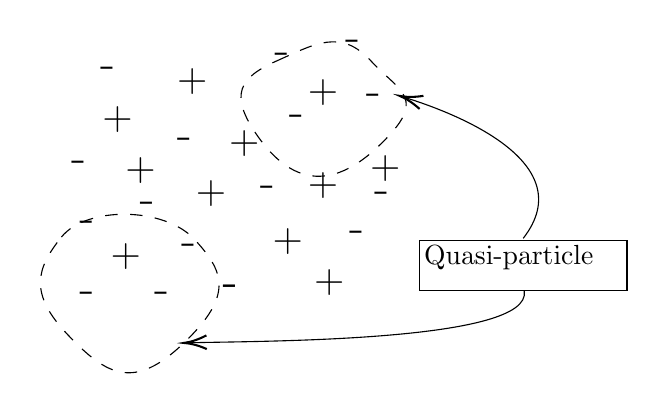
\begin{tikzpicture}[x=0.75pt,y=0.75pt,yscale=-1,xscale=1]
%uncomment if require: \path (0,300); %set diagram left start at 0, and has height of 300

%Shape: Polygon Curved [id:ds393267198766974] 
\draw  [dash pattern={on 4.5pt off 4.5pt}] (104.52,151.27) .. controls (116.52,136.27) and (154.03,136.65) .. (168.52,152.27) .. controls (183,167.88) and (187.52,179.27) .. (163.52,202.27) .. controls (139.52,225.27) and (126.52,218.27) .. (107.52,198.27) .. controls (88.52,178.27) and (92.52,166.27) .. (104.52,151.27) -- cycle ;
%Shape: Polygon Curved [id:ds5938648082047331] 
\draw  [dash pattern={on 4.5pt off 4.5pt}] (208.52,66.27) .. controls (226.52,58.27) and (239.03,50.65) .. (253.52,66.27) .. controls (268,81.88) and (281.52,84.27) .. (257.52,107.27) .. controls (233.52,130.27) and (214.52,124.27) .. (199.52,103.27) .. controls (184.52,82.27) and (190.52,74.27) .. (208.52,66.27) -- cycle ;
%Curve Lines [id:da7350178540870457] 
\draw    (327,151.88) .. controls (354.95,116) and (296.92,92.23) .. (269.18,83.77) ;
\draw [shift={(267.52,83.27)}, rotate = 376.5] [color={rgb, 255:red, 0; green, 0; blue, 0 }  ][line width=0.75]    (10.93,-3.29) .. controls (6.95,-1.4) and (3.31,-0.3) .. (0,0) .. controls (3.31,0.3) and (6.95,1.4) .. (10.93,3.29)   ;
%Curve Lines [id:da8754807282204362] 
\draw    (327.52,177.27) .. controls (331.46,201.89) and (200.54,201.29) .. (165.07,202.22) ;
\draw [shift={(163.52,202.27)}, rotate = 358.26] [color={rgb, 255:red, 0; green, 0; blue, 0 }  ][line width=0.75]    (10.93,-3.29) .. controls (6.95,-1.4) and (3.31,-0.3) .. (0,0) .. controls (3.31,0.3) and (6.95,1.4) .. (10.93,3.29)   ;

% Text Node
\draw (127,152.88) node [anchor=north west][inner sep=0.75pt]  [font=\Large] [align=left] {+};
% Text Node
\draw (141,128.88) node [anchor=north west][inner sep=0.75pt]  [font=\LARGE] [align=left] {\mbox{-}};
% Text Node
\draw (161,148.88) node [anchor=north west][inner sep=0.75pt]  [font=\LARGE] [align=left] {\mbox{-}};
% Text Node
\draw (148,171.88) node [anchor=north west][inner sep=0.75pt]  [font=\LARGE] [align=left] {\mbox{-}};
% Text Node
\draw (112,171.88) node [anchor=north west][inner sep=0.75pt]  [font=\LARGE] [align=left] {\mbox{-}};
% Text Node
\draw (112,137.88) node [anchor=north west][inner sep=0.75pt]  [font=\LARGE] [align=left] {\mbox{-}};
% Text Node
\draw (168,122.88) node [anchor=north west][inner sep=0.75pt]  [font=\Large] [align=left] {+};
% Text Node
\draw (205,145.88) node [anchor=north west][inner sep=0.75pt]  [font=\Large] [align=left] {+};
% Text Node
\draw (181,168.88) node [anchor=north west][inner sep=0.75pt]  [font=\LARGE] [align=left] {\mbox{-}};
% Text Node
\draw (181,168.88) node [anchor=north west][inner sep=0.75pt]  [font=\LARGE] [align=left] {\mbox{-}};
% Text Node
\draw (242,142.88) node [anchor=north west][inner sep=0.75pt]  [font=\LARGE] [align=left] {\mbox{-}};
% Text Node
\draw (199,120.88) node [anchor=north west][inner sep=0.75pt]  [font=\LARGE] [align=left] {\mbox{-}};
% Text Node
\draw (222,118.88) node [anchor=north west][inner sep=0.75pt]  [font=\Large] [align=left] {+};
% Text Node
\draw (184,98.88) node [anchor=north west][inner sep=0.75pt]  [font=\Large] [align=left] {+};
% Text Node
\draw (159,97.88) node [anchor=north west][inner sep=0.75pt]  [font=\LARGE] [align=left] {\mbox{-}};
% Text Node
\draw (254,123.88) node [anchor=north west][inner sep=0.75pt]  [font=\LARGE] [align=left] {\mbox{-}};
% Text Node
\draw (213,86.88) node [anchor=north west][inner sep=0.75pt]  [font=\LARGE] [align=left] {\mbox{-}};
% Text Node
\draw (250,76.88) node [anchor=north west][inner sep=0.75pt]  [font=\LARGE] [align=left] {\mbox{-}};
% Text Node
\draw (206,56.88) node [anchor=north west][inner sep=0.75pt]  [font=\LARGE] [align=left] {\mbox{-}};
% Text Node
\draw (240,50.88) node [anchor=north west][inner sep=0.75pt]  [font=\LARGE] [align=left] {\mbox{-}};
% Text Node
\draw (252,110.88) node [anchor=north west][inner sep=0.75pt]  [font=\Large] [align=left] {+};
% Text Node
\draw (222,73.88) node [anchor=north west][inner sep=0.75pt]  [font=\Large] [align=left] {+};
% Text Node
\draw (225,165.88) node [anchor=north west][inner sep=0.75pt]  [font=\Large] [align=left] {+};
% Text Node
\draw (159,68.88) node [anchor=north west][inner sep=0.75pt]  [font=\Large] [align=left] {+};
% Text Node
\draw (123,86.88) node [anchor=north west][inner sep=0.75pt]  [font=\Large] [align=left] {+};
% Text Node
\draw (108,108.88) node [anchor=north west][inner sep=0.75pt]  [font=\LARGE] [align=left] {\mbox{-}};
% Text Node
\draw (122,63.88) node [anchor=north west][inner sep=0.75pt]  [font=\LARGE] [align=left] {\mbox{-}};
% Text Node
\draw (134,111.88) node [anchor=north west][inner sep=0.75pt]  [font=\Large] [align=left] {+};
% Text Node
\draw    (277,152.88) -- (377,152.88) -- (377,176.88) -- (277,176.88) -- cycle  ;
\draw (278,153.88) node [anchor=north west][inner sep=0.75pt]   [align=left] {Quasi-particle};


\end{tikzpicture}

    \caption{Quasi particles in a Liquid of Positive and Negative Ions}
    \label{fig:quasi-particle-example}
\end{figure}
From Fig.\ref{fig:quasi-particle-example}, we know, from more powerful terminology of QFT:
\begin{center}
    "bare" particle + "clothing"/"cloud" = "dressed"/"renormalized" particle
\end{center}
For example, in quantum electrodynamics a 'bare' electron interacting with a field of photons acquires a cloud of virtual photons around it, converting it into the 'dressed' electron. In a similar manner, the interaction between real particles is called the 'bare' interaction, while the weak interaction between quasi particles is referred to as the 'effective' or "dressed" or "renormalized" interaction. \bluep{It should be noted that each bare particle is simultaneously the 'core' of a quasi particle and a transient 'member' of the cloud of several other quasi particles.}

The free quasi particles have a new energy law as 
$$\epsilon^{\prime}=\frac{p^{2}}{2 m^{*}} \quad \text { instead of } \quad \epsilon=\frac{p^{2}}{2 m}$$
where $m^*$ is the effective mass. The difference 
$$\epsilon_{quasi}-\epsilon_{bare}=\epsilon_{self}$$
is called \redp{\textbf{"self-energy"}} of the quasi particle.

@ Quantum System: quasi electreon in electron gas

The ' electron gas' is a simple model often used to describe many-body effects in metals. It consists of a box containing a large number of electrons interacting by means of the Coulomb force. In addition, there is a uniform, fixed, positive charge 'background' put into the box in order to keep the whole system electrically neutral. In the ground state, the electrons are spread out uniformly in the box.

Suppose now that we have a single, well-localized electron which we shoot into the electron gas  Because of the repulsive Coulomb interaction
between electrons, this extra electron repels other electrons away from it, so we get an empty space near the extra electron, and repelled electrons further away(Fig.\ref{fig:quasi-particle-example2}). This empty region may be viewed in a more detailed or microscopic way as composed of \redp{'holes'} in the electron gas. That is, the extra electron has "lifted out" electrons from the uniform charge distribution in its vicinity, thus creating 'holes' in this charge distribution, and has 'put down' these lifted-out electrons further away.
\begin{figure}[H]
    \centering
\tikzset {_0o14ioo3g/.code = {\pgfsetadditionalshadetransform{ \pgftransformshift{\pgfpoint{0 bp } { 0 bp }  }  \pgftransformscale{1 }  }}}
\pgfdeclareradialshading{_73ww2zakf}{\pgfpoint{0bp}{0bp}}{rgb(0bp)=(1,1,1);
rgb(12.019342694963727bp)=(1,1,1);
rgb(25bp)=(0,0,0);
rgb(400bp)=(0,0,0)}
\tikzset{_98ggw9slw/.code = {\pgfsetadditionalshadetransform{\pgftransformshift{\pgfpoint{0 bp } { 0 bp }  }  \pgftransformscale{1 } }}}
\pgfdeclareradialshading{_52d0oeat9} { \pgfpoint{0bp} {0bp}} {color(0bp)=(transparent!0);
color(12.019342694963727bp)=(transparent!0);
color(25bp)=(transparent!10);
color(400bp)=(transparent!10)} 
\pgfdeclarefading{_yzsmf2mqd}{\tikz \fill[shading=_52d0oeat9,_98ggw9slw] (0,0) rectangle (50bp,50bp); } 
\tikzset{every picture/.style={line width=0.75pt}} %set default line width to 0.75pt        

\begin{tikzpicture}[x=0.75pt,y=0.75pt,yscale=-1,xscale=1]
%uncomment if require: \path (0,300); %set diagram left start at 0, and has height of 300

%Shape: Rectangle [id:dp842398765103643] 
\draw  [fill={rgb, 255:red, 0; green, 0; blue, 0 }  ,fill opacity=1 ] (59.93,58.88) -- (235.32,58.88) -- (235.32,203.27) -- (59.93,203.27) -- cycle ;
%Shape: Circle [id:dp5878809314291961] 
\path  [shading=_73ww2zakf,_0o14ioo3g,path fading= _yzsmf2mqd ,fading transform={xshift=2}] (85.93,145.54) .. controls (85.93,131.37) and (97.42,119.88) .. (111.59,119.88) .. controls (125.76,119.88) and (137.25,131.37) .. (137.25,145.54) .. controls (137.25,159.71) and (125.76,171.2) .. (111.59,171.2) .. controls (97.42,171.2) and (85.93,159.71) .. (85.93,145.54) -- cycle ; % for fading 
 \draw   (85.93,145.54) .. controls (85.93,131.37) and (97.42,119.88) .. (111.59,119.88) .. controls (125.76,119.88) and (137.25,131.37) .. (137.25,145.54) .. controls (137.25,159.71) and (125.76,171.2) .. (111.59,171.2) .. controls (97.42,171.2) and (85.93,159.71) .. (85.93,145.54) -- cycle ; % for border 

%Shape: Circle [id:dp649192880176533] 
\draw  [fill={rgb, 255:red, 0; green, 0; blue, 0 }  ,fill opacity=1 ] (104.47,145.54) .. controls (104.47,141.61) and (107.66,138.42) .. (111.59,138.42) .. controls (115.53,138.42) and (118.72,141.61) .. (118.72,145.54) .. controls (118.72,149.48) and (115.53,152.67) .. (111.59,152.67) .. controls (107.66,152.67) and (104.47,149.48) .. (104.47,145.54) -- cycle ;
%Straight Lines [id:da47546531201986364] 
\draw [color={rgb, 255:red, 232; green, 30; blue, 12 }  ,draw opacity=1 ][line width=1.5]    (111.59,145.54) -- (135.11,122.37) ;
\draw [shift={(137.25,120.27)}, rotate = 495.43] [color={rgb, 255:red, 232; green, 30; blue, 12 }  ,draw opacity=1 ][line width=1.5]    (14.21,-4.28) .. controls (9.04,-1.82) and (4.3,-0.39) .. (0,0) .. controls (4.3,0.39) and (9.04,1.82) .. (14.21,4.28)   ;
%Shape: Rectangle [id:dp08609024153608191] 
\draw  [fill={rgb, 255:red, 0; green, 0; blue, 0 }  ,fill opacity=1 ] (261.93,58.88) -- (437.32,58.88) -- (437.32,203.27) -- (261.93,203.27) -- cycle ;
%Shape: Circle [id:dp8820237303823028] 
\draw  [fill={rgb, 255:red, 255; green, 255; blue, 255 }  ,fill opacity=1 ] (291,140.51) .. controls (291,136.3) and (294.41,132.88) .. (298.63,132.88) .. controls (302.84,132.88) and (306.25,136.3) .. (306.25,140.51) .. controls (306.25,144.72) and (302.84,148.13) .. (298.63,148.13) .. controls (294.41,148.13) and (291,144.72) .. (291,140.51) -- cycle ;
%Shape: Circle [id:dp5770389827427272] 
\draw  [fill={rgb, 255:red, 255; green, 255; blue, 255 }  ,fill opacity=1 ] (307,152.51) .. controls (307,148.3) and (310.41,144.88) .. (314.63,144.88) .. controls (318.84,144.88) and (322.25,148.3) .. (322.25,152.51) .. controls (322.25,156.72) and (318.84,160.13) .. (314.63,160.13) .. controls (310.41,160.13) and (307,156.72) .. (307,152.51) -- cycle ;
%Shape: Circle [id:dp025362450260817182] 
\draw  [fill={rgb, 255:red, 255; green, 255; blue, 255 }  ,fill opacity=1 ] (297,168.51) .. controls (297,164.3) and (300.41,160.88) .. (304.63,160.88) .. controls (308.84,160.88) and (312.25,164.3) .. (312.25,168.51) .. controls (312.25,172.72) and (308.84,176.13) .. (304.63,176.13) .. controls (300.41,176.13) and (297,172.72) .. (297,168.51) -- cycle ;
%Shape: Circle [id:dp9389847020012084] 
\draw  [fill={rgb, 255:red, 255; green, 255; blue, 255 }  ,fill opacity=1 ] (281,158.51) .. controls (281,154.3) and (284.41,150.88) .. (288.63,150.88) .. controls (292.84,150.88) and (296.25,154.3) .. (296.25,158.51) .. controls (296.25,162.72) and (292.84,166.13) .. (288.63,166.13) .. controls (284.41,166.13) and (281,162.72) .. (281,158.51) -- cycle ;
%Straight Lines [id:da4209538731972077] 
\draw [color={rgb, 255:red, 232; green, 30; blue, 12 }  ,draw opacity=1 ][line width=1.5]    (298.63,140.51) -- (293.85,117.21) ;
\draw [shift={(293.25,114.27)}, rotate = 438.42] [color={rgb, 255:red, 232; green, 30; blue, 12 }  ,draw opacity=1 ][line width=1.5]    (14.21,-4.28) .. controls (9.04,-1.82) and (4.3,-0.39) .. (0,0) .. controls (4.3,0.39) and (9.04,1.82) .. (14.21,4.28)   ;
%Straight Lines [id:da6368743975733171] 
\draw [color={rgb, 255:red, 232; green, 30; blue, 12 }  ,draw opacity=1 ][line width=1.5]    (314.63,152.51) -- (338.31,147.85) ;
\draw [shift={(341.25,147.27)}, rotate = 528.86] [color={rgb, 255:red, 232; green, 30; blue, 12 }  ,draw opacity=1 ][line width=1.5]    (14.21,-4.28) .. controls (9.04,-1.82) and (4.3,-0.39) .. (0,0) .. controls (4.3,0.39) and (9.04,1.82) .. (14.21,4.28)   ;
%Straight Lines [id:da3789740110796589] 
\draw [color={rgb, 255:red, 232; green, 30; blue, 12 }  ,draw opacity=1 ][line width=1.5]    (304.63,168.51) -- (322.7,179.69) ;
\draw [shift={(325.25,181.27)}, rotate = 211.74] [color={rgb, 255:red, 232; green, 30; blue, 12 }  ,draw opacity=1 ][line width=1.5]    (14.21,-4.28) .. controls (9.04,-1.82) and (4.3,-0.39) .. (0,0) .. controls (4.3,0.39) and (9.04,1.82) .. (14.21,4.28)   ;
%Straight Lines [id:da1630717526737726] 
\draw [color={rgb, 255:red, 232; green, 30; blue, 12 }  ,draw opacity=1 ][line width=1.5]    (288.63,158.51) -- (272.53,172.31) ;
\draw [shift={(270.25,174.27)}, rotate = 319.38] [color={rgb, 255:red, 232; green, 30; blue, 12 }  ,draw opacity=1 ][line width=1.5]    (14.21,-4.28) .. controls (9.04,-1.82) and (4.3,-0.39) .. (0,0) .. controls (4.3,0.39) and (9.04,1.82) .. (14.21,4.28)   ;

% Text Node
\draw (256,212.88) node [anchor=north west][inner sep=0.75pt]  [font=\footnotesize] [align=left] {(b)Lifted-out electrons create "holes"};
% Text Node
\draw (36,212.88) node [anchor=north west][inner sep=0.75pt]  [font=\footnotesize] [align=left] {(a)"Empty" region near the electron};


\end{tikzpicture}
    \caption{Extra Electron Pushes Other Electrons Away}
    \label{fig:quasi-particle-example2}
\end{figure}

@ Bogoliubov quasi particles ("bogolons")

These are the elementary excitations in a superconductor. We include them here since they are called quasi particles, but actually their structure is quite different from the 'particle plus cloud' picture described above. They consist of a linear combination ofan electron in state $(+k, \uparrow)$ and a hole $^{\prime}$ in $(-k, \downarrow)$.

\end{easylist}

\subsection{A Brief Intro to Collective Excitations}
As we have seen, the quasi particle consists of the original real, individual particle, plus a cloud of disturbed neighbours. It behaves very much like an
individual particle, except that it has an effective mass and a lifetime. But there also exist other kinds of fictitious particles in many-body systems, i.e., 'collective excitations'. These do not centre around individual particles, but instead involve collective, wavelike motion of all the particles in the system
simultaneously. Here are some examples:
\begin{easylist}
\NewList
@ Plasmons

If a thin metal foil is bombarded with high energy electrons, it is possible to set up sinusoidal oscillations in the density of the electron gas in the foil. This is known as a \bluep{'plasma wave'}, and it has a frequency $\omega_p$ and wavelength $\lambda_p$. \bluep{The plasma wave may be visualized as built up of 'holes' in the low-density regions and extra electrons in the high-density regions}. Just as light waves are quantized into units having energy $E=\hbar \omega$ called photons, plasma waves are quantized into units with energy $E_{p}=\hbar \omega_{p}$ called plasmons.

@ phonons

Sound waves are sinusoidal oscillations in the crystal lattice ofa solid. They are quantized into collective excitations called 'phonons'.

@ Magnons

In ferromagnets there are regular fluctuations in the density of spin angular momentum known as spin waves. The collective excitation here is the spin
wave quantum known as the 'magnon".
\end{easylist}

\subsection{Propagators-the Keys to the Many-body Problem}
The idea behind the propagator method is this: the detailed description of a many-body system requires in the classical case the position of each particle as a function of time, or in the quantum case, the time dependent wave function of the whole system. Fortunately, it turns out that \textbf{in order to find the important physical properties of a system it is not necessary to know the detailed behaviour of each particle in the system, but rather just the average behaviour of one or two typical particles.} \bluep{The quantities which describe this average behaviour are the\textit{ one-particle propagator} and \textit{two-particle propagator} respectively, and physical properties may be calculated directly from them.}

\begin{imp}
\textbf{One-particle propagator}: we put a particle into the interacting system at point $r_{1}$ at time $t_{1}$ and let it move through the system colliding with the other particles for a while (i.e., let it "propagate" through the system). Then the one-particle propagator is the probability (or in quantum systems, the probability amplitude) that the particle will be observed at the point $r_{2}$ at time $t_{2} .$ (Note that instead of putting the particle in at a definite point, it is sometimes more convenient to put it in with definite momentum, say $p_{1},$ and observe it later with momentum $p_{2} .$ ) \bluep{The single-particle propagator yields directly the energies and lifetimes of quasi particles. It also gives the momentum distribution, spin and particle density and can be used to calculate the ground state energy.}
\end{imp}
\begin{imp}
\textbf{Two-particle propagator}: the probability amplitude for observing one particle at $r_{2}, t_{2}$ and another at $r_{4}, t_{4}$ if one was put into the system at $r_{1}, t_{1}$ and another at $r_{3}, t_{3}$. This also has a wide variety of talents, \bluep{giving directly the energies and lifetimes of collective excitations, as well as the magnetic susceptibility, electrical conductivity, and a host of other non-cquilibrium properties.}
\end{imp}

\subsection{Calculate Propagator:the drunk man example}
With the aid of Feynman diagrams, we expand the propagator in an infinite series and evaluate the series approximately. This can be carried out in a general, systematic, and picturesque way.

Just to get an idea of what these diagrams are, consider the following simple example. A man who has had too much to drink, leaves a party at point 1 and on the way to his home at point 2, he can stop off at one or more bars-Alice's Bar (A), Bardot Bar (B), Club Six Bar (C), ... , etc. He can wind up either at his own home 2, or at any one of his friends' apartments, 3, 4, etc. We ask for the probability, P(2, I), that he gets home. This probability, which is just the propagator here (with time omitted for simplicity), is the sum of the probabilities for all the different ways he can propagate from I to 2 interacting with the various bars.

The first way he can prophgate is ' freely' from 1 to 2, i.e., without stopping at a bar. Call the probability for this free propagation $P_{0}(2,1)$

The second way he can propagate is to go freely from 1 to bar $A$ (the probability for this is $P_{0}(A, 1)$ ), then stop off at bar $A$ for a drink (call the probability for this $P(A))$, then go freely from $A$ to 2 (probability $=P_{0}(2, A)$ ). Assume for simplicity that the three processes here are independent. Then the total probability for this second way is the product of the probabilities for each process taken separately, i.e., $P_{0}(A, 1) \times P(A) \times P_{0}(2, A) .$ (This is like the case in coin-tossing: since each toss is independent, the probability of first tossing a head, then a tail, equals the probability of tossing a head times the probability of tossing a tail.)

The third way he can propagate is from 1 to $B$ to $2,$ with probability $P_{0}(B, 1) P(B) P_{0}(2, B) .$ Or he could go from 1 to $C$ to $2,$ etc., or from 1 to $A$ to $B$ to $2,$ or from 1 to $A,$ come out of $A,$ go back into $A,$ then go to $2,$ and so on. The total probability, $P(2,1)$ is then given by the sum of the probabilities for each way, i.e., the infinite series:
$$\begin{aligned}
P(2,1)=&P_{0}(2,1)+P_{0}(A, 1) P(A) P_{0}(2, A)+P_{0}(B, 1) P(B) P_{0}(2, B)+\cdots  \\
&+P_{0}(A, 1) P(A) P_{0}(B, A) P(B) P_{0}(2, B)+\cdots
\end{aligned}$$
\redp{This is an example of a 'perturbation series', since each interaction with a bar "perturbs" the free propagation of the drunken man.} Represent this series using the following dictionary:
\begin{figure}[H]
    \centering
\tikzset{every picture/.style={line width=0.75pt}} %set default line width to 0.75pt        

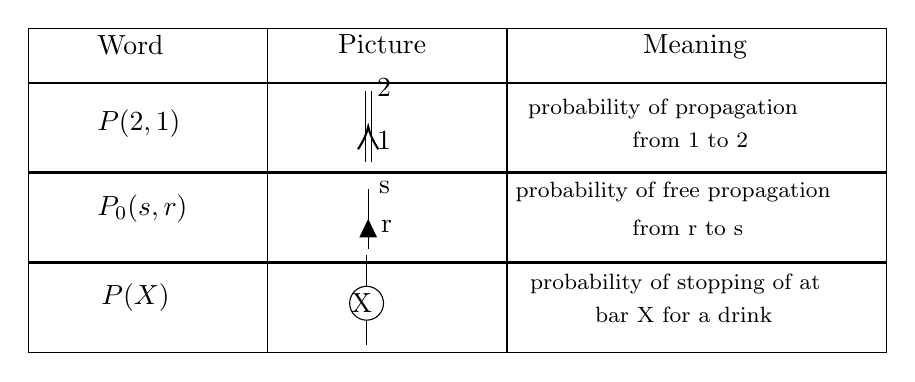
\begin{tikzpicture}[x=0.75pt,y=0.75pt,yscale=-1,xscale=1]
%uncomment if require: \path (0,349); %set diagram left start at 0, and has height of 349

%Shape: Rectangle [id:dp3972753239553969] 
\draw   (212.78,159.32) -- (328.11,159.32) -- (328.11,185.7) -- (212.78,185.7) -- cycle ;
%Shape: Rectangle [id:dp013530620031451002] 
\draw   (328.11,159.32) -- (443.44,159.32) -- (443.44,185.7) -- (328.11,185.7) -- cycle ;
%Shape: Rectangle [id:dp736076383888415] 
\draw   (443.44,159.32) -- (626.17,159.32) -- (626.17,185.7) -- (443.44,185.7) -- cycle ;
%Shape: Rectangle [id:dp018483080609867475] 
\draw   (212.78,185.32) -- (328.11,185.32) -- (328.11,229.2) -- (212.78,229.2) -- cycle ;
%Shape: Rectangle [id:dp18336509171990412] 
\draw   (328.11,185.32) -- (443.44,185.32) -- (443.44,229.2) -- (328.11,229.2) -- cycle ;
%Shape: Rectangle [id:dp5452879627568872] 
\draw   (443.44,185.32) -- (626.17,185.32) -- (626.17,229.2) -- (443.44,229.2) -- cycle ;
%Shape: Rectangle [id:dp710141061414926] 
\draw   (212.78,228.57) -- (328.11,228.57) -- (328.11,272.45) -- (212.78,272.45) -- cycle ;
%Shape: Rectangle [id:dp6981715844716105] 
\draw   (328.11,228.57) -- (443.44,228.57) -- (443.44,272.45) -- (328.11,272.45) -- cycle ;
%Shape: Rectangle [id:dp9707206740138988] 
\draw   (443.44,228.57) -- (626.17,228.57) -- (626.17,272.45) -- (443.44,272.45) -- cycle ;
%Shape: Rectangle [id:dp7188406169431831] 
\draw   (212.78,271.81) -- (328.11,271.81) -- (328.11,315.7) -- (212.78,315.7) -- cycle ;
%Shape: Rectangle [id:dp35373677352561617] 
\draw   (328.11,271.81) -- (443.44,271.81) -- (443.44,315.7) -- (328.11,315.7) -- cycle ;
%Shape: Rectangle [id:dp7761518007990666] 
\draw   (443.44,271.81) -- (626.17,271.81) -- (626.17,315.7) -- (443.44,315.7) -- cycle ;
%Straight Lines [id:da3953067075421305] 
\draw    (375.07,223.7) -- (375.07,189.7)(378.07,223.7) -- (378.07,189.7) ;
\draw [shift={(376.57,206.7)}, rotate = 450] [color={rgb, 255:red, 0; green, 0; blue, 0 }  ][line width=0.75]    (10.93,-4.9) .. controls (6.95,-2.3) and (3.31,-0.67) .. (0,0) .. controls (3.31,0.67) and (6.95,2.3) .. (10.93,4.9)   ;
%Straight Lines [id:da5701847229817978] 
\draw    (376.57,265.7) -- (376.57,236.7) ;
\draw [shift={(376.57,251.2)}, rotate = 450] [fill={rgb, 255:red, 0; green, 0; blue, 0 }  ][line width=0.08]  [draw opacity=0] (8.93,-4.29) -- (0,0) -- (8.93,4.29) -- cycle    ;
%Shape: Ellipse [id:dp16063069982491784] 
\draw   (367.64,291.82) .. controls (367.64,287.31) and (371.29,283.66) .. (375.79,283.66) .. controls (380.3,283.66) and (383.95,287.31) .. (383.95,291.82) .. controls (383.95,296.32) and (380.3,299.97) .. (375.79,299.97) .. controls (371.29,299.97) and (367.64,296.32) .. (367.64,291.82) -- cycle ;
%Straight Lines [id:da2549697012881261] 
\draw    (375.79,283.66) -- (375.79,268.7) ;
%Straight Lines [id:da05824951890975272] 
\draw    (375.79,311.7) -- (375.79,299.97) ;

% Text Node
\draw (244.78,161.32) node [anchor=north west][inner sep=0.75pt]   [align=left] {Word};
% Text Node
\draw (360.78,161.32) node [anchor=north west][inner sep=0.75pt]   [align=left] {Picture};
% Text Node
\draw (507.78,161.32) node [anchor=north west][inner sep=0.75pt]   [align=left] {Meaning};
% Text Node
\draw (244.78,197.32) node [anchor=north west][inner sep=0.75pt]    {$P( 2,1)$};
% Text Node
\draw (379.57,207.76) node [anchor=north west][inner sep=0.75pt]   [align=left] {1};
% Text Node
\draw (379.57,182.54) node [anchor=north west][inner sep=0.75pt]   [align=left] {2};
% Text Node
\draw (244.78,238.32) node [anchor=north west][inner sep=0.75pt]    {$P_{0}( s,r)$};
% Text Node
\draw (381.57,250.76) node [anchor=north west][inner sep=0.75pt]   [align=left] {r};
% Text Node
\draw (380.57,231.7) node [anchor=north west][inner sep=0.75pt]   [align=left] {s};
% Text Node
\draw (367.2,285.75) node [anchor=north west][inner sep=0.75pt]   [align=left] {X};
% Text Node
\draw (246.78,281.32) node [anchor=north west][inner sep=0.75pt]    {$P( X)$};
% Text Node
\draw (452.33,192.32) node [anchor=north west][inner sep=0.75pt]  [font=\footnotesize] [align=left] {probability of propagation };
% Text Node
\draw (502.63,208.32) node [anchor=north west][inner sep=0.75pt]  [font=\footnotesize] [align=left] {from 1 to 2};
% Text Node
\draw (446.33,232.32) node [anchor=north west][inner sep=0.75pt]  [font=\footnotesize] [align=left] {probability of free propagation };
% Text Node
\draw (502.63,250.32) node [anchor=north west][inner sep=0.75pt]  [font=\footnotesize] [align=left] {from r to s};
% Text Node
\draw (453.33,276.32) node [anchor=north west][inner sep=0.75pt]  [font=\footnotesize] [align=left] {probability of stopping of at \ };
% Text Node
\draw (484.63,292.32) node [anchor=north west][inner sep=0.75pt]  [font=\footnotesize] [align=left] {bar X for a drink};


\end{tikzpicture}

    \caption{Diagram dictionary for drunken man}
    \label{fig:drunken-man-1}
\end{figure}
The perturbation series in diagrams for this drunken man propagator is therefore
\begin{figure}[H]
    \centering
    


\tikzset{every picture/.style={line width=0.75pt}} %set default line width to 0.75pt        

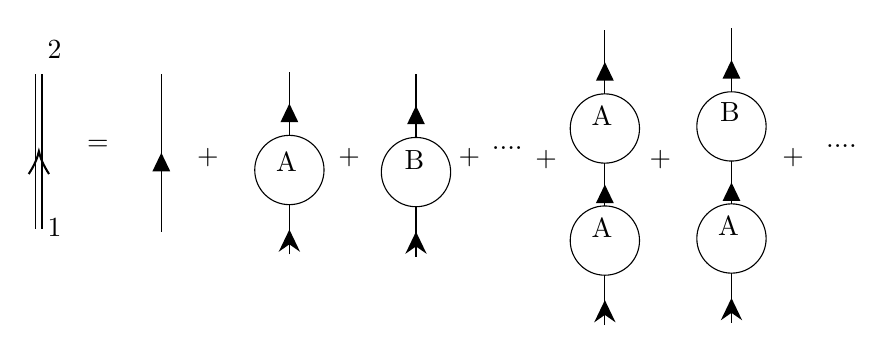
\begin{tikzpicture}[x=0.75pt,y=0.75pt,yscale=-1,xscale=1]
%uncomment if require: \path (0,349); %set diagram left start at 0, and has height of 349

%Straight Lines [id:da4757935872975344] 
\draw    (8.07,101.32) -- (8.07,26.7)(11.07,101.32) -- (11.07,26.7) ;
\draw [shift={(9.57,64.01)}, rotate = 450] [color={rgb, 255:red, 0; green, 0; blue, 0 }  ][line width=0.75]    (10.93,-4.9) .. controls (6.95,-2.3) and (3.31,-0.67) .. (0,0) .. controls (3.31,0.67) and (6.95,2.3) .. (10.93,4.9)   ;
%Straight Lines [id:da23622371172830803] 
\draw    (68.57,102.7) -- (68.57,26.7) ;
\draw [shift={(68.57,64.7)}, rotate = 450] [fill={rgb, 255:red, 0; green, 0; blue, 0 }  ][line width=0.08]  [draw opacity=0] (8.93,-4.29) -- (0,0) -- (8.93,4.29) -- cycle    ;
%Shape: Circle [id:dp4139523862436749] 
\draw   (113.57,73.01) .. controls (113.57,63.79) and (121.04,56.32) .. (130.26,56.32) .. controls (139.48,56.32) and (146.95,63.79) .. (146.95,73.01) .. controls (146.95,82.23) and (139.48,89.7) .. (130.26,89.7) .. controls (121.04,89.7) and (113.57,82.23) .. (113.57,73.01) -- cycle ;
%Straight Lines [id:da33169967910609544] 
\draw    (130.26,56.32) -- (130.26,25.7) ;
\draw [shift={(130.26,41.01)}, rotate = 450] [fill={rgb, 255:red, 0; green, 0; blue, 0 }  ][line width=0.08]  [draw opacity=0] (8.93,-4.29) -- (0,0) -- (8.93,4.29) -- cycle    ;
%Straight Lines [id:da28347419222198567] 
\draw    (130.26,113.7) -- (130.26,89.7) ;
\draw [shift={(130.26,101.7)}, rotate = 450] [fill={rgb, 255:red, 0; green, 0; blue, 0 }  ][line width=0.08]  [draw opacity=0] (10.72,-5.15) -- (0,0) -- (10.72,5.15) -- (7.12,0) -- cycle    ;
%Shape: Circle [id:dp1723289826034129] 
\draw   (174.57,74.01) .. controls (174.57,64.79) and (182.04,57.32) .. (191.26,57.32) .. controls (200.48,57.32) and (207.95,64.79) .. (207.95,74.01) .. controls (207.95,83.23) and (200.48,90.7) .. (191.26,90.7) .. controls (182.04,90.7) and (174.57,83.23) .. (174.57,74.01) -- cycle ;
%Straight Lines [id:da40381754331686626] 
\draw    (191.26,57.32) -- (191.26,26.7) ;
\draw [shift={(191.26,42.01)}, rotate = 450] [fill={rgb, 255:red, 0; green, 0; blue, 0 }  ][line width=0.08]  [draw opacity=0] (8.93,-4.29) -- (0,0) -- (8.93,4.29) -- cycle    ;
%Straight Lines [id:da5172106067784763] 
\draw    (191.26,114.7) -- (191.26,90.7) ;
\draw [shift={(191.26,102.7)}, rotate = 450] [fill={rgb, 255:red, 0; green, 0; blue, 0 }  ][line width=0.08]  [draw opacity=0] (10.72,-5.15) -- (0,0) -- (10.72,5.15) -- (7.12,0) -- cycle    ;
%Shape: Circle [id:dp663325870350397] 
\draw   (265.57,107.01) .. controls (265.57,97.79) and (273.04,90.32) .. (282.26,90.32) .. controls (291.48,90.32) and (298.95,97.79) .. (298.95,107.01) .. controls (298.95,116.23) and (291.48,123.7) .. (282.26,123.7) .. controls (273.04,123.7) and (265.57,116.23) .. (265.57,107.01) -- cycle ;
%Straight Lines [id:da6913773132395338] 
\draw    (282.26,36.32) -- (282.26,5.7) ;
\draw [shift={(282.26,21.01)}, rotate = 450] [fill={rgb, 255:red, 0; green, 0; blue, 0 }  ][line width=0.08]  [draw opacity=0] (8.93,-4.29) -- (0,0) -- (8.93,4.29) -- cycle    ;
%Straight Lines [id:da4724377841227787] 
\draw    (282.26,147.7) -- (282.26,123.7) ;
\draw [shift={(282.26,135.7)}, rotate = 450] [fill={rgb, 255:red, 0; green, 0; blue, 0 }  ][line width=0.08]  [draw opacity=0] (10.72,-5.15) -- (0,0) -- (10.72,5.15) -- (7.12,0) -- cycle    ;
%Shape: Circle [id:dp29262051024858293] 
\draw   (265.57,53.01) .. controls (265.57,43.79) and (273.04,36.32) .. (282.26,36.32) .. controls (291.48,36.32) and (298.95,43.79) .. (298.95,53.01) .. controls (298.95,62.23) and (291.48,69.7) .. (282.26,69.7) .. controls (273.04,69.7) and (265.57,62.23) .. (265.57,53.01) -- cycle ;
%Straight Lines [id:da2293551017015375] 
\draw    (282.26,69.7) -- (282.26,90.32) ;
\draw [shift={(282.26,80.01)}, rotate = 90] [fill={rgb, 255:red, 0; green, 0; blue, 0 }  ][line width=0.08]  [draw opacity=0] (8.93,-4.29) -- (0,0) -- (8.93,4.29) -- cycle    ;
%Shape: Circle [id:dp5742274191772756] 
\draw   (326.57,106.01) .. controls (326.57,96.79) and (334.04,89.32) .. (343.26,89.32) .. controls (352.48,89.32) and (359.95,96.79) .. (359.95,106.01) .. controls (359.95,115.23) and (352.48,122.7) .. (343.26,122.7) .. controls (334.04,122.7) and (326.57,115.23) .. (326.57,106.01) -- cycle ;
%Straight Lines [id:da8337372469854066] 
\draw    (343.26,35.32) -- (343.26,4.7) ;
\draw [shift={(343.26,20.01)}, rotate = 450] [fill={rgb, 255:red, 0; green, 0; blue, 0 }  ][line width=0.08]  [draw opacity=0] (8.93,-4.29) -- (0,0) -- (8.93,4.29) -- cycle    ;
%Straight Lines [id:da42712440571211296] 
\draw    (343.26,146.7) -- (343.26,122.7) ;
\draw [shift={(343.26,134.7)}, rotate = 450] [fill={rgb, 255:red, 0; green, 0; blue, 0 }  ][line width=0.08]  [draw opacity=0] (10.72,-5.15) -- (0,0) -- (10.72,5.15) -- (7.12,0) -- cycle    ;
%Shape: Circle [id:dp5287893719741432] 
\draw   (326.57,52.01) .. controls (326.57,42.79) and (334.04,35.32) .. (343.26,35.32) .. controls (352.48,35.32) and (359.95,42.79) .. (359.95,52.01) .. controls (359.95,61.23) and (352.48,68.7) .. (343.26,68.7) .. controls (334.04,68.7) and (326.57,61.23) .. (326.57,52.01) -- cycle ;
%Straight Lines [id:da8377025286119076] 
\draw    (343.26,68.7) -- (343.26,89.32) ;
\draw [shift={(343.26,79.01)}, rotate = 90] [fill={rgb, 255:red, 0; green, 0; blue, 0 }  ][line width=0.08]  [draw opacity=0] (8.93,-4.29) -- (0,0) -- (8.93,4.29) -- cycle    ;

% Text Node
\draw (12.57,95.32) node [anchor=north west][inner sep=0.75pt]   [align=left] {1};
% Text Node
\draw (12.57,9.32) node [anchor=north west][inner sep=0.75pt]   [align=left] {2};
% Text Node
\draw (31.57,57.32) node [anchor=north west][inner sep=0.75pt]   [align=left] {=};
% Text Node
\draw (122.57,63.32) node [anchor=north west][inner sep=0.75pt]   [align=left] {A};
% Text Node
\draw (184.57,62.32) node [anchor=north west][inner sep=0.75pt]   [align=left] {B};
% Text Node
\draw (336.57,39.32) node [anchor=north west][inner sep=0.75pt]   [align=left] {B};
% Text Node
\draw (335.57,94.32) node [anchor=north west][inner sep=0.75pt]   [align=left] {A};
% Text Node
\draw (274.57,95.32) node [anchor=north west][inner sep=0.75pt]   [align=left] {A};
% Text Node
\draw (274.57,41.32) node [anchor=north west][inner sep=0.75pt]   [align=left] {A};
% Text Node
\draw (84.57,61.32) node [anchor=north west][inner sep=0.75pt]    {$+$};
% Text Node
\draw (152.57,61.32) node [anchor=north west][inner sep=0.75pt]    {$+$};
% Text Node
\draw (210.57,61.32) node [anchor=north west][inner sep=0.75pt]    {$+$};
% Text Node
\draw (226.57,60.32) node [anchor=north west][inner sep=0.75pt]   [align=left] {....};
% Text Node
\draw (247.57,62.32) node [anchor=north west][inner sep=0.75pt]    {$+$};
% Text Node
\draw (302.57,62.32) node [anchor=north west][inner sep=0.75pt]    {$+$};
% Text Node
\draw (366.57,61.32) node [anchor=north west][inner sep=0.75pt]    {$+$};
% Text Node
\draw (387.57,59.32) node [anchor=north west][inner sep=0.75pt]   [align=left] {....};


\end{tikzpicture}

    \caption{Drunken man series}
    \label{fig:drunken-man-2}
\end{figure}

\subsection{Single-particle propagator for system of many interacting particles}
We now describe a second-order propagation process as following:
\begin{itemize}
    \item At time $t_1$, extra particle enters system
    \item At time t, extra particle interacts with a particle (through virtual photon) in the system, lifting it out of its place, creating a "hole" in the system
    \item The extra particle, plus the "hole" and the "lifted-out" particle(\redp{particle-hole pair}) travel through the system
    \item At time $t^{\prime}$, the extra particle interacts with  "lifted-out" particle, knocking it back into the hole, thus destroying the particle-hole pair.
    \item At time $t_2$, the extra particle moves out of the system.
\end{itemize}
We use the following diagram elements here.\bluep{Note that the hole is drawn as a particle moving backward in time}.
\begin{figure}[H]
    \centering
\tikzset{every picture/.style={line width=0.75pt}} %set default line width to 0.75pt        

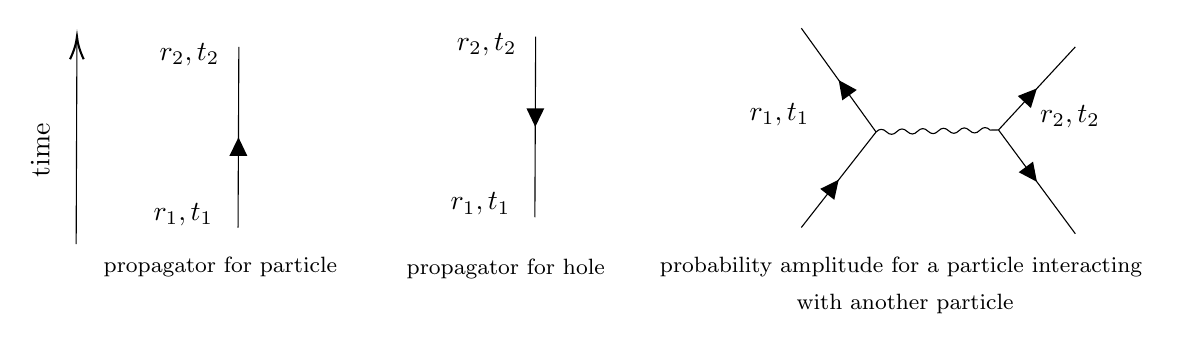
\begin{tikzpicture}[x=0.75pt,y=0.75pt,yscale=-1,xscale=1]
%uncomment if require: \path (0,300); %set diagram left start at 0, and has height of 300

%Straight Lines [id:da19133695979745402] 
\draw    (190.28,120) -- (190.67,32.93) ;
\draw [shift={(190.48,76.47)}, rotate = 450.25] [fill={rgb, 255:red, 0; green, 0; blue, 0 }  ][line width=0.08]  [draw opacity=0] (8.93,-4.29) -- (0,0) -- (8.93,4.29) -- cycle    ;
%Straight Lines [id:da8918233616398107] 
\draw    (112.28,128) -- (112.66,29.93) ;
\draw [shift={(112.67,27.93)}, rotate = 450.22] [color={rgb, 255:red, 0; green, 0; blue, 0 }  ][line width=0.75]    (10.93,-3.29) .. controls (6.95,-1.4) and (3.31,-0.3) .. (0,0) .. controls (3.31,0.3) and (6.95,1.4) .. (10.93,3.29)   ;
%Straight Lines [id:da9519966290540162] 
\draw    (333.29,115) -- (333.67,27.93) ;
\draw [shift={(333.48,71.47)}, rotate = 270.25] [fill={rgb, 255:red, 0; green, 0; blue, 0 }  ][line width=0.08]  [draw opacity=0] (8.93,-4.29) -- (0,0) -- (8.93,4.29) -- cycle    ;
%Straight Lines [id:da7312209816881998] 
\draw    (593.67,122.93) -- (556.67,72.93) ;
\draw [shift={(575.17,97.93)}, rotate = 233.5] [fill={rgb, 255:red, 0; green, 0; blue, 0 }  ][line width=0.08]  [draw opacity=0] (8.93,-4.29) -- (0,0) -- (8.93,4.29) -- cycle    ;
%Straight Lines [id:da37095749047846227] 
\draw    (593.67,32.93) -- (556.67,72.93) ;
\draw [shift={(575.17,52.93)}, rotate = 132.77] [fill={rgb, 255:red, 0; green, 0; blue, 0 }  ][line width=0.08]  [draw opacity=0] (8.93,-4.29) -- (0,0) -- (8.93,4.29) -- cycle    ;
%Straight Lines [id:da18873008311254413] 
\draw    (497.67,73.93) -- (461.67,23.93) ;
\draw [shift={(479.67,48.93)}, rotate = 414.25] [fill={rgb, 255:red, 0; green, 0; blue, 0 }  ][line width=0.08]  [draw opacity=0] (8.93,-4.29) -- (0,0) -- (8.93,4.29) -- cycle    ;
%Straight Lines [id:da6044480912830338] 
\draw    (497.67,73.93) -- (461.67,119.93) ;
\draw [shift={(479.67,96.93)}, rotate = 128.05] [fill={rgb, 255:red, 0; green, 0; blue, 0 }  ][line width=0.08]  [draw opacity=0] (8.93,-4.29) -- (0,0) -- (8.93,4.29) -- cycle    ;
%Straight Lines [id:da35473256420919863] 
\draw    (497.67,73.93) .. controls (499.31,72.24) and (500.98,72.21) .. (502.67,73.85) .. controls (504.36,75.48) and (506.03,75.45) .. (507.67,73.76) .. controls (509.3,72.07) and (510.97,72.04) .. (512.66,73.68) .. controls (514.35,75.31) and (516.02,75.28) .. (517.66,73.59) .. controls (519.3,71.9) and (520.97,71.87) .. (522.66,73.51) .. controls (524.35,75.14) and (526.02,75.11) .. (527.66,73.42) .. controls (529.3,71.73) and (530.97,71.7) .. (532.66,73.34) .. controls (534.35,74.98) and (536.02,74.95) .. (537.66,73.26) .. controls (539.3,71.57) and (540.97,71.54) .. (542.66,73.17) .. controls (544.35,74.81) and (546.02,74.78) .. (547.66,73.09) .. controls (549.3,71.4) and (550.97,71.37) .. (552.66,73) -- (556.67,72.93) -- (556.67,72.93) ;

% Text Node
\draw (89.19,96.94) node [anchor=north west][inner sep=0.75pt]  [rotate=-270.31] [align=left] {time};
% Text Node
\draw (148.28,107) node [anchor=north west][inner sep=0.75pt]    {$r_{1} ,t_{1}$};
% Text Node
\draw (151.28,30) node [anchor=north west][inner sep=0.75pt]    {$r_{2} ,t_{2}$};
% Text Node
\draw (124.28,133) node [anchor=north west][inner sep=0.75pt]  [font=\footnotesize] [align=left] {propagator for particle};
% Text Node
\draw (291.49,102) node [anchor=north west][inner sep=0.75pt]    {$r_{1} ,t_{1}$};
% Text Node
\draw (294.46,25) node [anchor=north west][inner sep=0.75pt]    {$r_{2} ,t_{2}$};
% Text Node
\draw (270.28,134) node [anchor=north west][inner sep=0.75pt]  [font=\footnotesize] [align=left] {propagator for hole};
% Text Node
\draw (435.49,59) node [anchor=north west][inner sep=0.75pt]    {$r_{1} ,t_{1}$};
% Text Node
\draw (575.46,60) node [anchor=north west][inner sep=0.75pt]    {$r_{2} ,t_{2}$};
% Text Node
\draw (392.28,133) node [anchor=north west][inner sep=0.75pt]  [font=\footnotesize] [align=left] {probability amplitude for a particle interacting };
% Text Node
\draw (458.13,151) node [anchor=north west][inner sep=0.75pt]  [font=\footnotesize] [align=left] {with another particle};


\end{tikzpicture}

    \caption{Diagram elements for second-order propagation}
    \label{fig:elem-2nd-propagator}
\end{figure}
Then the probability amplitude for the above sequence of events can be represented by the diagram
\begin{center}
\tikzset{every picture/.style={line width=0.75pt}} %set default line width to 0.75pt        

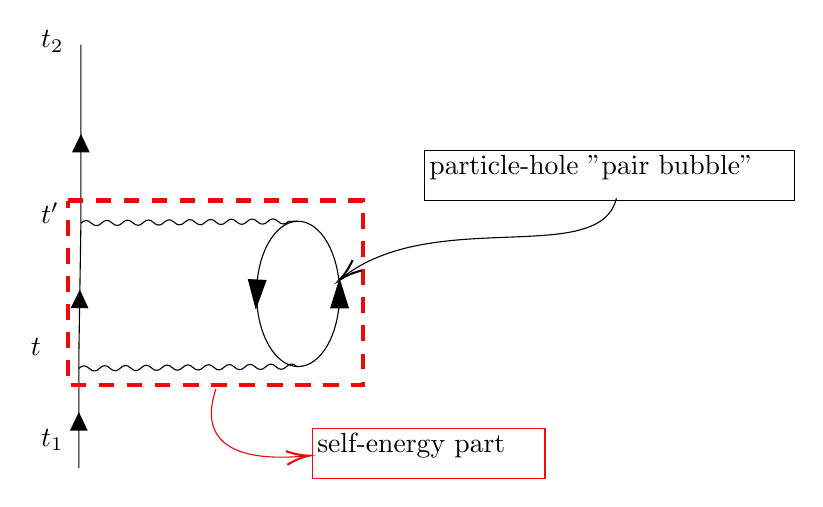
\begin{tikzpicture}[x=0.75pt,y=0.75pt,yscale=-1,xscale=1]
%uncomment if require: \path (0,300); %set diagram left start at 0, and has height of 300

%Straight Lines [id:da3914578805076815] 
\draw    (239.9,40.93) -- (239.9,126.93) -- (238.9,190.93) -- (238.9,244.93) ;
\draw [shift={(239.9,83.93)}, rotate = 90] [fill={rgb, 255:red, 0; green, 0; blue, 0 }  ][line width=0.08]  [draw opacity=0] (8.93,-4.29) -- (0,0) -- (8.93,4.29) -- cycle    ;
\draw [shift={(239.4,158.93)}, rotate = 90.9] [fill={rgb, 255:red, 0; green, 0; blue, 0 }  ][line width=0.08]  [draw opacity=0] (8.93,-4.29) -- (0,0) -- (8.93,4.29) -- cycle    ;
\draw [shift={(238.9,217.93)}, rotate = 90] [fill={rgb, 255:red, 0; green, 0; blue, 0 }  ][line width=0.08]  [draw opacity=0] (8.93,-4.29) -- (0,0) -- (8.93,4.29) -- cycle    ;
%Shape: Ellipse [id:dp4458035019540618] 
\draw   (344.57,196) .. controls (333.53,196.02) and (324.55,180.36) .. (324.52,161.03) .. controls (324.49,141.7) and (333.42,126.02) .. (344.46,126) .. controls (355.51,125.98) and (364.49,141.64) .. (364.52,160.97) .. controls (364.55,180.3) and (355.62,195.98) .. (344.57,196) -- cycle ;
%Straight Lines [id:da03751642849998316] 
\draw    (239.9,126.93) .. controls (241.55,125.25) and (243.22,125.24) .. (244.9,126.89) .. controls (246.58,128.54) and (248.25,128.52) .. (249.9,126.84) .. controls (251.55,125.16) and (253.22,125.15) .. (254.9,126.8) .. controls (256.58,128.45) and (258.25,128.43) .. (259.9,126.75) .. controls (261.55,125.07) and (263.22,125.06) .. (264.9,126.71) .. controls (266.58,128.36) and (268.25,128.35) .. (269.9,126.67) .. controls (271.55,124.99) and (273.22,124.97) .. (274.9,126.62) .. controls (276.58,128.27) and (278.25,128.26) .. (279.9,126.58) .. controls (281.55,124.9) and (283.22,124.88) .. (284.9,126.53) .. controls (286.58,128.18) and (288.25,128.17) .. (289.9,126.49) .. controls (291.55,124.81) and (293.22,124.79) .. (294.9,126.44) .. controls (296.58,128.09) and (298.25,128.08) .. (299.9,126.4) .. controls (301.55,124.72) and (303.22,124.7) .. (304.9,126.35) .. controls (306.58,128) and (308.25,127.99) .. (309.9,126.31) .. controls (311.55,124.63) and (313.22,124.61) .. (314.9,126.26) .. controls (316.58,127.91) and (318.25,127.9) .. (319.9,126.22) .. controls (321.55,124.54) and (323.22,124.52) .. (324.9,126.17) .. controls (326.58,127.82) and (328.25,127.81) .. (329.9,126.13) .. controls (331.55,124.45) and (333.22,124.44) .. (334.9,126.09) .. controls (336.58,127.74) and (338.25,127.72) .. (339.9,126.04) -- (344.46,126) -- (344.46,126) ;
%Straight Lines [id:da22386446930432802] 
\draw    (238.9,196.93) .. controls (240.55,195.25) and (242.22,195.24) .. (243.9,196.89) .. controls (245.58,198.54) and (247.25,198.53) .. (248.9,196.85) .. controls (250.55,195.17) and (252.22,195.15) .. (253.9,196.8) .. controls (255.58,198.45) and (257.25,198.44) .. (258.9,196.76) .. controls (260.55,195.08) and (262.22,195.06) .. (263.9,196.71) .. controls (265.58,198.36) and (267.25,198.35) .. (268.9,196.67) .. controls (270.55,194.99) and (272.22,194.97) .. (273.9,196.62) .. controls (275.58,198.27) and (277.25,198.26) .. (278.9,196.58) .. controls (280.55,194.9) and (282.22,194.89) .. (283.9,196.54) .. controls (285.58,198.19) and (287.25,198.17) .. (288.9,196.49) .. controls (290.55,194.81) and (292.22,194.8) .. (293.9,196.45) .. controls (295.58,198.1) and (297.25,198.08) .. (298.9,196.4) .. controls (300.55,194.72) and (302.22,194.71) .. (303.9,196.36) .. controls (305.58,198.01) and (307.25,198) .. (308.9,196.32) .. controls (310.55,194.64) and (312.22,194.62) .. (313.9,196.27) .. controls (315.58,197.92) and (317.25,197.91) .. (318.9,196.23) .. controls (320.55,194.55) and (322.22,194.53) .. (323.9,196.18) .. controls (325.58,197.83) and (327.25,197.82) .. (328.9,196.14) .. controls (330.55,194.46) and (332.22,194.44) .. (333.9,196.09) .. controls (335.58,197.74) and (337.25,197.73) .. (338.9,196.05) .. controls (340.55,194.37) and (342.22,194.36) .. (343.9,196.01) -- (344.57,196) -- (344.57,196) ;
%Shape: Triangle [id:dp8438251936972118] 
\draw  [fill={rgb, 255:red, 0; green, 0; blue, 0 }  ,fill opacity=1 ] (364.52,154.25) -- (368.71,167.68) -- (360.32,167.68) -- cycle ;
%Shape: Triangle [id:dp13261991584446953] 
\draw  [fill={rgb, 255:red, 0; green, 0; blue, 0 }  ,fill opacity=1 ] (324.2,167.74) -- (320.64,154.13) -- (329.02,154.52) -- cycle ;
%Shape: Rectangle [id:dp26500062559360993] 
\draw  [color={rgb, 255:red, 239; green, 9; blue, 9 }  ,draw opacity=1 ][dash pattern={on 5.63pt off 4.5pt}][line width=1.5]  (233.52,116) -- (375.9,116) -- (375.9,204.93) -- (233.52,204.93) -- cycle ;
%Curve Lines [id:da7889824653675461] 
\draw [color={rgb, 255:red, 233; green, 8; blue, 8 }  ,draw opacity=1 ]   (304.9,206.93) .. controls (297.02,230.57) and (310.86,242.51) .. (348.18,239.1) ;
\draw [shift={(349.9,238.93)}, rotate = 534.1800000000001] [color={rgb, 255:red, 233; green, 8; blue, 8 }  ,draw opacity=1 ][line width=0.75]    (10.93,-3.29) .. controls (6.95,-1.4) and (3.31,-0.3) .. (0,0) .. controls (3.31,0.3) and (6.95,1.4) .. (10.93,3.29)   ;
%Curve Lines [id:da8696448552998278] 
\draw    (497.9,114.93) .. controls (489.98,148.59) and (409.53,118.55) .. (365.83,153.18) ;
\draw [shift={(364.52,154.25)}, rotate = 320.06] [color={rgb, 255:red, 0; green, 0; blue, 0 }  ][line width=0.75]    (10.93,-3.29) .. controls (6.95,-1.4) and (3.31,-0.3) .. (0,0) .. controls (3.31,0.3) and (6.95,1.4) .. (10.93,3.29)   ;

% Text Node
\draw (219.52,225) node [anchor=north west][inner sep=0.75pt]    {$t_{1}$};
% Text Node
\draw (214.52,181) node [anchor=north west][inner sep=0.75pt]    {$t$};
% Text Node
\draw (219.52,116) node [anchor=north west][inner sep=0.75pt]    {$t^{\prime }$};
% Text Node
\draw (219.52,33) node [anchor=north west][inner sep=0.75pt]    {$t_{2}$};
% Text Node
\draw  [color={rgb, 255:red, 244; green, 10; blue, 10 }  ,draw opacity=1 ]  (351.52,226) -- (463.52,226) -- (463.52,250) -- (351.52,250) -- cycle  ;
\draw (352.52,227) node [anchor=north west][inner sep=0.75pt]   [align=left] {self-energy part};
% Text Node
\draw    (405.52,92) -- (583.52,92) -- (583.52,116) -- (405.52,116) -- cycle  ;
\draw (406.52,93) node [anchor=north west][inner sep=0.75pt]   [align=left] {particle-hole "pair bubble"};


\end{tikzpicture}

\end{center}
where we have a so-called "self-energy part" because it shows the particle interacting with itself via the particle-hole pair it created in the many-body medium.

Another sequence of events which can occur involves only one interaction (i.e., a 'first-order ' process). It is a \bluep{quick-change act in which the incoming electron at point r interacts with another electron at point r' and changes place with it}. This is analogous to billiard ball 1 striking billiard ball 2 and transferring all its momentum to 2. The process sequence is:
\begin{itemize}
    \item Extra particle enters at time $t_1$
    \item At time $t$, the particles is at point $r$. It interacts with a particle at $r^{\prime}$(through virtual photon) and changes place with it.
    \item Extra particle leaves at time $t_2$
\end{itemize}
with a "open oyster" diagram as below:
\begin{center}
    


\tikzset{every picture/.style={line width=0.75pt}} %set default line width to 0.75pt        

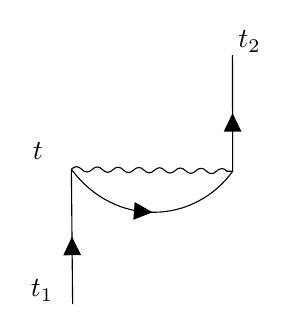
\begin{tikzpicture}[x=0.75pt,y=0.75pt,yscale=-1,xscale=1]
%uncomment if require: \path (0,300); %set diagram left start at 0, and has height of 300

%Curve Lines [id:da7645811334291478] 
\draw    (486.9,124.93) .. controls (507.62,152.93) and (545.62,151.93) .. (564.62,125.93) ;
\draw [shift={(525.97,145.68)}, rotate = 184.29] [fill={rgb, 255:red, 0; green, 0; blue, 0 }  ][line width=0.08]  [draw opacity=0] (8.93,-4.29) -- (0,0) -- (8.93,4.29) -- cycle    ;
%Straight Lines [id:da0067325630711646545] 
\draw    (486.9,124.93) -- (487.5,189.93) ;
\draw [shift={(487.2,157.43)}, rotate = 89.47] [fill={rgb, 255:red, 0; green, 0; blue, 0 }  ][line width=0.08]  [draw opacity=0] (8.93,-4.29) -- (0,0) -- (8.93,4.29) -- cycle    ;
%Straight Lines [id:da31755570766840036] 
\draw    (486.9,124.93) .. controls (488.59,123.29) and (490.25,123.31) .. (491.9,125) .. controls (493.55,126.69) and (495.21,126.71) .. (496.9,125.06) .. controls (498.59,123.42) and (500.25,123.44) .. (501.9,125.13) .. controls (503.55,126.82) and (505.21,126.84) .. (506.9,125.19) .. controls (508.59,123.54) and (510.25,123.56) .. (511.9,125.25) .. controls (513.55,126.94) and (515.21,126.96) .. (516.9,125.32) .. controls (518.59,123.67) and (520.25,123.69) .. (521.9,125.38) .. controls (523.55,127.07) and (525.21,127.09) .. (526.9,125.45) .. controls (528.59,123.8) and (530.25,123.82) .. (531.9,125.51) .. controls (533.55,127.2) and (535.21,127.22) .. (536.9,125.58) .. controls (538.59,123.93) and (540.25,123.95) .. (541.9,125.64) .. controls (543.55,127.33) and (545.21,127.35) .. (546.9,125.71) .. controls (548.59,124.06) and (550.25,124.08) .. (551.89,125.77) .. controls (553.54,127.46) and (555.2,127.48) .. (556.89,125.83) .. controls (558.58,124.19) and (560.24,124.21) .. (561.89,125.9) -- (564.62,125.93) -- (564.62,125.93) ;
%Straight Lines [id:da6864724196774904] 
\draw    (564.62,125.93) -- (564.5,69.93) ;
\draw [shift={(564.56,97.93)}, rotate = 449.88] [fill={rgb, 255:red, 0; green, 0; blue, 0 }  ][line width=0.08]  [draw opacity=0] (8.93,-4.29) -- (0,0) -- (8.93,4.29) -- cycle    ;

% Text Node
\draw (466.12,177) node [anchor=north west][inner sep=0.75pt]    {$t_{1}$};
% Text Node
\draw (566.12,57) node [anchor=north west][inner sep=0.75pt]    {$t_{2}$};
% Text Node
\draw (467.12,111) node [anchor=north west][inner sep=0.75pt]    {$t$};


\end{tikzpicture}
\end{center}

We can see the direct connection between the one-particle propagator and the quasi particle by looking at all the diagrams at a particular time $t_0$ (dashed line)
\begin{center}

\tikzset{every picture/.style={line width=0.75pt}} %set default line width to 0.75pt        

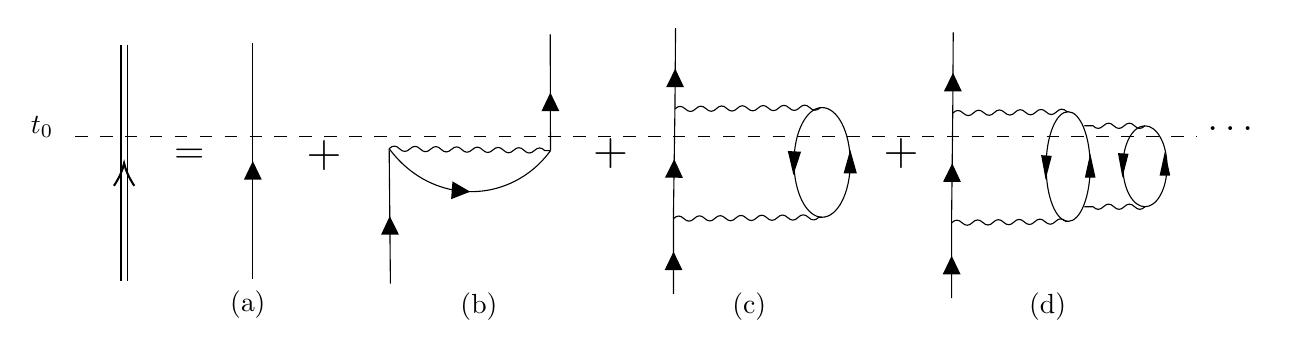
\begin{tikzpicture}[x=0.75pt,y=0.75pt,yscale=-1,xscale=1]
%uncomment if require: \path (0,300); %set diagram left start at 0, and has height of 300

%Straight Lines [id:da3914578805076815] 
\draw    (343.88,60.93) -- (343.58,99.85) -- (342.9,148.17) -- (342.9,188.93) ;
\draw [shift={(343.73,80.39)}, rotate = 90.45] [fill={rgb, 255:red, 0; green, 0; blue, 0 }  ][line width=0.08]  [draw opacity=0] (8.93,-4.29) -- (0,0) -- (8.93,4.29) -- cycle    ;
\draw [shift={(343.24,124.01)}, rotate = 90.8] [fill={rgb, 255:red, 0; green, 0; blue, 0 }  ][line width=0.08]  [draw opacity=0] (8.93,-4.29) -- (0,0) -- (8.93,4.29) -- cycle    ;
\draw [shift={(342.9,168.55)}, rotate = 90] [fill={rgb, 255:red, 0; green, 0; blue, 0 }  ][line width=0.08]  [draw opacity=0] (8.93,-4.29) -- (0,0) -- (8.93,4.29) -- cycle    ;
%Shape: Ellipse [id:dp4458035019540618] 
\draw   (414.52,151.99) .. controls (407.04,152.01) and (400.95,140.19) .. (400.93,125.6) .. controls (400.91,111) and (406.96,99.16) .. (414.45,99.15) .. controls (421.94,99.14) and (428.02,110.96) .. (428.04,125.55) .. controls (428.06,140.14) and (422.01,151.98) .. (414.52,151.99) -- cycle ;
%Straight Lines [id:da03751642849998316] 
\draw    (343.58,99.85) .. controls (345.23,98.17) and (346.9,98.16) .. (348.58,99.81) .. controls (350.26,101.46) and (351.93,101.44) .. (353.58,99.76) .. controls (355.23,98.08) and (356.9,98.06) .. (358.58,99.71) .. controls (360.26,101.36) and (361.93,101.34) .. (363.58,99.66) .. controls (365.23,97.98) and (366.9,97.96) .. (368.58,99.61) .. controls (370.26,101.26) and (371.93,101.24) .. (373.58,99.56) .. controls (375.23,97.88) and (376.9,97.86) .. (378.58,99.51) .. controls (380.26,101.16) and (381.93,101.14) .. (383.58,99.46) .. controls (385.23,97.78) and (386.9,97.76) .. (388.58,99.41) .. controls (390.26,101.06) and (391.93,101.04) .. (393.58,99.36) .. controls (395.23,97.68) and (396.9,97.66) .. (398.58,99.31) .. controls (400.26,100.96) and (401.92,100.94) .. (403.57,99.26) .. controls (405.22,97.58) and (406.89,97.56) .. (408.57,99.21) .. controls (410.25,100.86) and (411.92,100.84) .. (413.57,99.16) -- (414.45,99.15) -- (414.45,99.15) ;
%Straight Lines [id:da22386446930432802] 
\draw    (342.9,152.7) .. controls (344.55,151.01) and (346.22,151) .. (347.9,152.65) .. controls (349.58,154.3) and (351.25,154.28) .. (352.9,152.6) .. controls (354.55,150.92) and (356.22,150.9) .. (357.9,152.55) .. controls (359.58,154.2) and (361.25,154.18) .. (362.9,152.5) .. controls (364.55,150.82) and (366.22,150.8) .. (367.9,152.45) .. controls (369.58,154.1) and (371.25,154.08) .. (372.9,152.4) .. controls (374.55,150.72) and (376.22,150.7) .. (377.9,152.35) .. controls (379.58,154) and (381.25,153.98) .. (382.9,152.3) .. controls (384.55,150.62) and (386.22,150.61) .. (387.9,152.26) .. controls (389.58,153.91) and (391.25,153.89) .. (392.9,152.21) .. controls (394.55,150.53) and (396.22,150.51) .. (397.9,152.16) .. controls (399.58,153.81) and (401.25,153.79) .. (402.9,152.11) .. controls (404.55,150.43) and (406.22,150.41) .. (407.9,152.06) .. controls (409.58,153.71) and (411.25,153.69) .. (412.9,152.01) -- (414.52,151.99) -- (414.52,151.99) ;
%Shape: Triangle [id:dp8438251936972118] 
\draw  [fill={rgb, 255:red, 0; green, 0; blue, 0 }  ,fill opacity=1 ] (428.04,120.48) -- (430.88,130.62) -- (425.2,130.62) -- cycle ;
%Shape: Triangle [id:dp13261991584446953] 
\draw  [fill={rgb, 255:red, 0; green, 0; blue, 0 }  ,fill opacity=1 ] (400.72,130.66) -- (398.31,120.38) -- (403.98,120.68) -- cycle ;
%Curve Lines [id:da7645811334291478] 
\draw    (205.9,118.93) .. controls (226.62,146.93) and (264.62,145.93) .. (283.62,119.93) ;
\draw [shift={(244.97,139.68)}, rotate = 184.29] [fill={rgb, 255:red, 0; green, 0; blue, 0 }  ][line width=0.08]  [draw opacity=0] (8.93,-4.29) -- (0,0) -- (8.93,4.29) -- cycle    ;
%Straight Lines [id:da0067325630711646545] 
\draw    (205.9,118.93) -- (206.5,183.93) ;
\draw [shift={(206.2,151.43)}, rotate = 89.47] [fill={rgb, 255:red, 0; green, 0; blue, 0 }  ][line width=0.08]  [draw opacity=0] (8.93,-4.29) -- (0,0) -- (8.93,4.29) -- cycle    ;
%Straight Lines [id:da31755570766840036] 
\draw    (205.9,118.93) .. controls (207.59,117.29) and (209.25,117.31) .. (210.9,119) .. controls (212.55,120.69) and (214.21,120.71) .. (215.9,119.06) .. controls (217.59,117.42) and (219.25,117.44) .. (220.9,119.13) .. controls (222.55,120.82) and (224.21,120.84) .. (225.9,119.19) .. controls (227.59,117.54) and (229.25,117.56) .. (230.9,119.25) .. controls (232.55,120.94) and (234.21,120.96) .. (235.9,119.32) .. controls (237.59,117.67) and (239.25,117.69) .. (240.9,119.38) .. controls (242.55,121.07) and (244.21,121.09) .. (245.9,119.45) .. controls (247.59,117.8) and (249.25,117.82) .. (250.9,119.51) .. controls (252.55,121.2) and (254.21,121.22) .. (255.9,119.58) .. controls (257.59,117.93) and (259.25,117.95) .. (260.9,119.64) .. controls (262.55,121.33) and (264.21,121.35) .. (265.9,119.71) .. controls (267.59,118.06) and (269.25,118.08) .. (270.89,119.77) .. controls (272.54,121.46) and (274.2,121.48) .. (275.89,119.83) .. controls (277.58,118.19) and (279.24,118.21) .. (280.89,119.9) -- (283.62,119.93) -- (283.62,119.93) ;
%Straight Lines [id:da6864724196774904] 
\draw    (283.62,119.93) -- (283.5,63.93) ;
\draw [shift={(283.56,91.93)}, rotate = 449.88] [fill={rgb, 255:red, 0; green, 0; blue, 0 }  ][line width=0.08]  [draw opacity=0] (8.93,-4.29) -- (0,0) -- (8.93,4.29) -- cycle    ;
%Straight Lines [id:da0059350286742723135] 
\draw    (477.67,62.93) -- (477.43,101.85) -- (476.9,150.17) -- (476.9,190.93) ;
\draw [shift={(477.55,82.39)}, rotate = 90.35] [fill={rgb, 255:red, 0; green, 0; blue, 0 }  ][line width=0.08]  [draw opacity=0] (8.93,-4.29) -- (0,0) -- (8.93,4.29) -- cycle    ;
\draw [shift={(477.17,126.01)}, rotate = 90.63] [fill={rgb, 255:red, 0; green, 0; blue, 0 }  ][line width=0.08]  [draw opacity=0] (8.93,-4.29) -- (0,0) -- (8.93,4.29) -- cycle    ;
\draw [shift={(476.9,170.55)}, rotate = 90] [fill={rgb, 255:red, 0; green, 0; blue, 0 }  ][line width=0.08]  [draw opacity=0] (8.93,-4.29) -- (0,0) -- (8.93,4.29) -- cycle    ;
%Shape: Ellipse [id:dp1973299491754572] 
\draw   (533.05,153.99) .. controls (527.19,154.01) and (522.42,142.19) .. (522.4,127.6) .. controls (522.39,113) and (527.13,101.16) .. (533,101.15) .. controls (538.87,101.14) and (543.64,112.96) .. (543.65,127.55) .. controls (543.67,142.14) and (538.92,153.98) .. (533.05,153.99) -- cycle ;
%Straight Lines [id:da3221956834758286] 
\draw    (477.43,101.85) .. controls (479.08,100.16) and (480.74,100.14) .. (482.43,101.79) .. controls (484.12,103.44) and (485.78,103.42) .. (487.43,101.73) .. controls (489.08,100.04) and (490.74,100.02) .. (492.43,101.66) .. controls (494.12,103.31) and (495.78,103.29) .. (497.43,101.6) .. controls (499.08,99.91) and (500.74,99.89) .. (502.43,101.54) .. controls (504.12,103.18) and (505.78,103.16) .. (507.43,101.47) .. controls (509.08,99.78) and (510.74,99.76) .. (512.43,101.41) .. controls (514.12,103.06) and (515.78,103.04) .. (517.43,101.35) .. controls (519.08,99.66) and (520.74,99.64) .. (522.43,101.28) .. controls (524.12,102.93) and (525.78,102.91) .. (527.43,101.22) .. controls (529.08,99.53) and (530.74,99.51) .. (532.43,101.16) -- (533,101.15) -- (533,101.15) ;
%Straight Lines [id:da6584771753926739] 
\draw    (476.9,154.7) .. controls (478.55,153.01) and (480.21,152.99) .. (481.9,154.64) .. controls (483.59,156.28) and (485.25,156.26) .. (486.9,154.57) .. controls (488.55,152.88) and (490.21,152.86) .. (491.9,154.51) .. controls (493.59,156.16) and (495.25,156.14) .. (496.9,154.45) .. controls (498.55,152.76) and (500.21,152.74) .. (501.9,154.38) .. controls (503.59,156.03) and (505.25,156.01) .. (506.9,154.32) .. controls (508.55,152.63) and (510.21,152.61) .. (511.9,154.26) .. controls (513.59,155.91) and (515.25,155.89) .. (516.9,154.2) .. controls (518.55,152.51) and (520.21,152.49) .. (521.9,154.13) .. controls (523.59,155.78) and (525.25,155.76) .. (526.9,154.07) .. controls (528.55,152.38) and (530.21,152.36) .. (531.9,154.01) -- (533.06,153.99) -- (533.06,153.99) ;
%Shape: Triangle [id:dp5997188211998996] 
\draw  [fill={rgb, 255:red, 0; green, 0; blue, 0 }  ,fill opacity=1 ] (543.66,122.48) -- (545.88,132.62) -- (541.43,132.62) -- cycle ;
%Shape: Triangle [id:dp7955336974508751] 
\draw  [fill={rgb, 255:red, 0; green, 0; blue, 0 }  ,fill opacity=1 ] (522.23,132.66) -- (520.34,122.38) -- (524.79,122.68) -- cycle ;
%Shape: Ellipse [id:dp7587823287069684] 
\draw   (570.05,146.94) .. controls (564.18,146.95) and (559.41,138.23) .. (559.4,127.46) .. controls (559.39,116.69) and (564.14,107.95) .. (570.01,107.94) .. controls (575.87,107.92) and (580.64,116.64) .. (580.65,127.41) .. controls (580.66,138.18) and (575.92,146.92) .. (570.05,146.94) -- cycle ;
%Straight Lines [id:da9010071179516257] 
\draw    (570.01,107.94) .. controls (568.34,109.6) and (566.68,109.6) .. (565.01,107.93) .. controls (563.34,106.26) and (561.68,106.26) .. (560.01,107.93) .. controls (558.34,109.6) and (556.68,109.6) .. (555.01,107.93) .. controls (553.34,106.26) and (551.68,106.26) .. (550.01,107.93) .. controls (548.34,109.6) and (546.68,109.6) .. (545.01,107.93) -- (540.88,107.93) -- (540.88,107.93) ;
%Straight Lines [id:da039834872543490274] 
\draw    (570.05,146.94) .. controls (568.38,148.6) and (566.72,148.6) .. (565.05,146.93) .. controls (563.38,145.26) and (561.72,145.26) .. (560.05,146.93) .. controls (558.38,148.6) and (556.72,148.6) .. (555.05,146.93) .. controls (553.38,145.26) and (551.72,145.26) .. (550.05,146.93) .. controls (548.38,148.6) and (546.72,148.6) .. (545.05,146.93) -- (540.88,146.93) -- (540.88,146.93) ;
%Shape: Triangle [id:dp23179144168316745] 
\draw  [fill={rgb, 255:red, 0; green, 0; blue, 0 }  ,fill opacity=1 ] (579.66,121.48) -- (581.88,131.62) -- (577.43,131.62) -- cycle ;
%Shape: Triangle [id:dp5658762911563971] 
\draw  [fill={rgb, 255:red, 0; green, 0; blue, 0 }  ,fill opacity=1 ] (559.23,131.66) -- (557.34,121.38) -- (561.79,121.68) -- cycle ;
%Straight Lines [id:da298908695859174] 
\draw    (140.2,67.93) -- (140.2,181.93) ;
\draw [shift={(140.2,124.93)}, rotate = 90] [fill={rgb, 255:red, 0; green, 0; blue, 0 }  ][line width=0.08]  [draw opacity=0] (8.93,-4.29) -- (0,0) -- (8.93,4.29) -- cycle    ;
%Straight Lines [id:da2811220945791332] 
\draw    (79.7,68.93) -- (79.7,182.93)(76.7,68.93) -- (76.7,182.93) ;
\draw [shift={(78.2,125.93)}, rotate = 90] [color={rgb, 255:red, 0; green, 0; blue, 0 }  ][line width=0.75]    (10.93,-4.9) .. controls (6.95,-2.3) and (3.31,-0.67) .. (0,0) .. controls (3.31,0.67) and (6.95,2.3) .. (10.93,4.9)   ;
%Straight Lines [id:da7873018114908388] 
\draw  [dash pattern={on 4.5pt off 4.5pt}]  (54.63,113) -- (595.23,113) ;

% Text Node
\draw (101,118) node [anchor=north west][inner sep=0.75pt]  [font=\Large] [align=left] {=};
% Text Node
\draw (165,114) node [anchor=north west][inner sep=0.75pt]  [font=\LARGE] [align=left] {+};
% Text Node
\draw (303,113) node [anchor=north west][inner sep=0.75pt]  [font=\LARGE] [align=left] {+};
% Text Node
\draw (443,113) node [anchor=north west][inner sep=0.75pt]  [font=\LARGE] [align=left] {+};
% Text Node
\draw (598.85,107) node [anchor=north west][inner sep=0.75pt]  [font=\Large]  {$\dotsc $};
% Text Node
\draw (32,102) node [anchor=north west][inner sep=0.75pt]    {$t_{0}$};
% Text Node
\draw (128,186) node [anchor=north west][inner sep=0.75pt]   [align=left] {(a)};
% Text Node
\draw (239,187) node [anchor=north west][inner sep=0.75pt]   [align=left] {(b)};
% Text Node
\draw (370,187) node [anchor=north west][inner sep=0.75pt]   [align=left] {(c)};
% Text Node
\draw (513,187) node [anchor=north west][inner sep=0.75pt]   [align=left] {(d)};


\end{tikzpicture}
\end{center}
At $t_{0},$ we see that various situations may exist: there may be just the bare particle ( $a$ ), or there may exist two particles plus one hole created by the second order sequence ( $c$ ), or three particles plus two holes in $(d)$, etc. That is, the diagrams show all the configurations of particles and holes which may be kicked up by the bare particle as it churns through the many-body system. Thus, \textbf{the diagrams reveal the content of the ever-changing cloud of particles and holes surrounding the bare particle and converting it into a quasi particle.}


\subsection{The two-particle propagator and the particle-hole propagator}
The two-particle propagator is the sum over the probability amplitudes for all the ways two particles can enter the system, interact with each other and with the particles in the system, then emerge again. The diagram series for it is (note that the dots on the diagram for the two-particle propagator show the points at which directed lines emerge):
\begin{center}
    


\tikzset{every picture/.style={line width=0.75pt}} %set default line width to 0.75pt        

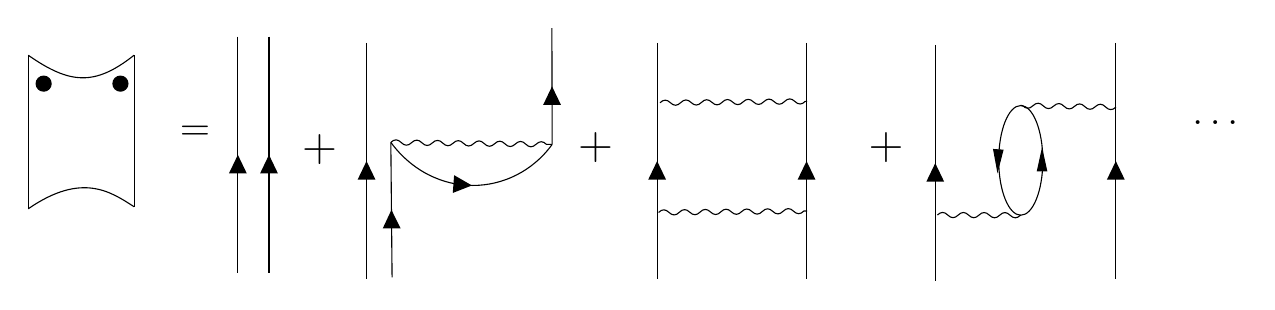
\begin{tikzpicture}[x=0.75pt,y=0.75pt,yscale=-1,xscale=1]
%uncomment if require: \path (0,300); %set diagram left start at 0, and has height of 300

%Straight Lines [id:da03751642849998316] 
\draw    (343.58,99.85) .. controls (345.23,98.17) and (346.9,98.16) .. (348.58,99.81) .. controls (350.26,101.46) and (351.93,101.44) .. (353.58,99.76) .. controls (355.23,98.08) and (356.9,98.06) .. (358.58,99.71) .. controls (360.26,101.36) and (361.93,101.34) .. (363.58,99.66) .. controls (365.23,97.98) and (366.9,97.96) .. (368.58,99.61) .. controls (370.26,101.26) and (371.93,101.24) .. (373.58,99.56) .. controls (375.23,97.88) and (376.9,97.86) .. (378.58,99.51) .. controls (380.26,101.16) and (381.93,101.14) .. (383.58,99.46) .. controls (385.23,97.78) and (386.9,97.76) .. (388.58,99.41) .. controls (390.26,101.06) and (391.93,101.04) .. (393.58,99.36) .. controls (395.23,97.68) and (396.9,97.66) .. (398.58,99.31) .. controls (400.26,100.96) and (401.92,100.94) .. (403.57,99.26) .. controls (405.22,97.58) and (406.89,97.56) .. (408.57,99.21) .. controls (410.25,100.86) and (411.92,100.84) .. (413.57,99.16) -- (414.45,99.15) -- (414.45,99.15) ;
%Straight Lines [id:da22386446930432802] 
\draw    (342.9,152.7) .. controls (344.55,151.01) and (346.22,151) .. (347.9,152.65) .. controls (349.58,154.3) and (351.25,154.28) .. (352.9,152.6) .. controls (354.55,150.92) and (356.22,150.9) .. (357.9,152.55) .. controls (359.58,154.2) and (361.25,154.18) .. (362.9,152.5) .. controls (364.55,150.82) and (366.22,150.8) .. (367.9,152.45) .. controls (369.58,154.1) and (371.25,154.08) .. (372.9,152.4) .. controls (374.55,150.72) and (376.22,150.7) .. (377.9,152.35) .. controls (379.58,154) and (381.25,153.98) .. (382.9,152.3) .. controls (384.55,150.62) and (386.22,150.61) .. (387.9,152.26) .. controls (389.58,153.91) and (391.25,153.89) .. (392.9,152.21) .. controls (394.55,150.53) and (396.22,150.51) .. (397.9,152.16) .. controls (399.58,153.81) and (401.25,153.79) .. (402.9,152.11) .. controls (404.55,150.43) and (406.22,150.41) .. (407.9,152.06) .. controls (409.58,153.71) and (411.25,153.69) .. (412.9,152.01) -- (414.52,151.99) -- (414.52,151.99) ;
%Curve Lines [id:da7645811334291478] 
\draw    (213.9,118.93) .. controls (234.62,146.93) and (272.62,145.93) .. (291.62,119.93) ;
\draw [shift={(252.97,139.68)}, rotate = 184.29] [fill={rgb, 255:red, 0; green, 0; blue, 0 }  ][line width=0.08]  [draw opacity=0] (8.93,-4.29) -- (0,0) -- (8.93,4.29) -- cycle    ;
%Straight Lines [id:da0067325630711646545] 
\draw    (213.9,118.93) -- (214.5,183.93) ;
\draw [shift={(214.2,151.43)}, rotate = 89.47] [fill={rgb, 255:red, 0; green, 0; blue, 0 }  ][line width=0.08]  [draw opacity=0] (8.93,-4.29) -- (0,0) -- (8.93,4.29) -- cycle    ;
%Straight Lines [id:da31755570766840036] 
\draw    (213.9,118.93) .. controls (215.59,117.29) and (217.25,117.31) .. (218.9,119) .. controls (220.55,120.69) and (222.21,120.71) .. (223.9,119.06) .. controls (225.59,117.42) and (227.25,117.44) .. (228.9,119.13) .. controls (230.55,120.82) and (232.21,120.84) .. (233.9,119.19) .. controls (235.59,117.54) and (237.25,117.56) .. (238.9,119.25) .. controls (240.55,120.94) and (242.21,120.96) .. (243.9,119.32) .. controls (245.59,117.67) and (247.25,117.69) .. (248.9,119.38) .. controls (250.55,121.07) and (252.21,121.09) .. (253.9,119.45) .. controls (255.59,117.8) and (257.25,117.82) .. (258.9,119.51) .. controls (260.55,121.2) and (262.21,121.22) .. (263.9,119.58) .. controls (265.59,117.93) and (267.25,117.95) .. (268.9,119.64) .. controls (270.55,121.33) and (272.21,121.35) .. (273.9,119.71) .. controls (275.59,118.06) and (277.25,118.08) .. (278.89,119.77) .. controls (280.54,121.46) and (282.2,121.48) .. (283.89,119.83) .. controls (285.58,118.19) and (287.24,118.21) .. (288.89,119.9) -- (291.62,119.93) -- (291.62,119.93) ;
%Straight Lines [id:da6864724196774904] 
\draw    (291.62,119.93) -- (291.5,63.93) ;
\draw [shift={(291.56,91.93)}, rotate = 449.88] [fill={rgb, 255:red, 0; green, 0; blue, 0 }  ][line width=0.08]  [draw opacity=0] (8.93,-4.29) -- (0,0) -- (8.93,4.29) -- cycle    ;
%Shape: Ellipse [id:dp1973299491754572] 
\draw   (517.43,154.02) .. controls (511.56,154.03) and (506.79,142.21) .. (506.77,127.62) .. controls (506.76,113.03) and (511.5,101.19) .. (517.37,101.17) .. controls (523.24,101.16) and (528.01,112.98) .. (528.03,127.57) .. controls (528.04,142.16) and (523.3,154) .. (517.43,154.02) -- cycle ;
%Straight Lines [id:da3221956834758286] 
\draw    (563.25,101.93) .. controls (561.56,103.57) and (559.89,103.54) .. (558.25,101.85) .. controls (556.61,100.16) and (554.94,100.13) .. (553.25,101.77) .. controls (551.56,103.41) and (549.89,103.38) .. (548.25,101.69) .. controls (546.61,100) and (544.94,99.97) .. (543.25,101.6) .. controls (541.56,103.24) and (539.89,103.21) .. (538.25,101.52) .. controls (536.61,99.83) and (534.94,99.8) .. (533.25,101.44) .. controls (531.56,103.07) and (529.89,103.04) .. (528.25,101.35) .. controls (526.62,99.66) and (524.95,99.63) .. (523.26,101.27) .. controls (521.57,102.91) and (519.9,102.88) .. (518.26,101.19) -- (517.37,101.17) -- (517.37,101.17) ;
%Straight Lines [id:da6584771753926739] 
\draw    (477.25,153.93) .. controls (478.92,152.27) and (480.58,152.27) .. (482.25,153.94) .. controls (483.92,155.61) and (485.58,155.61) .. (487.25,153.95) .. controls (488.92,152.29) and (490.58,152.29) .. (492.25,153.96) .. controls (493.92,155.63) and (495.58,155.63) .. (497.25,153.97) .. controls (498.92,152.31) and (500.59,152.32) .. (502.25,153.99) .. controls (503.92,155.66) and (505.58,155.66) .. (507.25,154) .. controls (508.92,152.34) and (510.58,152.34) .. (512.25,154.01) .. controls (513.92,155.68) and (515.58,155.68) .. (517.25,154.02) -- (517.43,154.02) -- (517.43,154.02) ;
%Shape: Triangle [id:dp5997188211998996] 
\draw  [fill={rgb, 255:red, 0; green, 0; blue, 0 }  ,fill opacity=1 ] (527.66,122.48) -- (529.88,132.62) -- (525.43,132.62) -- cycle ;
%Shape: Triangle [id:dp7955336974508751] 
\draw  [fill={rgb, 255:red, 0; green, 0; blue, 0 }  ,fill opacity=1 ] (506.23,132.66) -- (504.34,122.38) -- (508.79,122.68) -- cycle ;
%Straight Lines [id:da298908695859174] 
\draw    (140.2,67.93) -- (140.2,181.93) ;
\draw [shift={(140.2,124.93)}, rotate = 90] [fill={rgb, 255:red, 0; green, 0; blue, 0 }  ][line width=0.08]  [draw opacity=0] (8.93,-4.29) -- (0,0) -- (8.93,4.29) -- cycle    ;
%Straight Lines [id:da6974050351887592] 
\draw    (155.2,67.93) -- (155.2,181.93) ;
\draw [shift={(155.2,124.93)}, rotate = 90] [fill={rgb, 255:red, 0; green, 0; blue, 0 }  ][line width=0.08]  [draw opacity=0] (8.93,-4.29) -- (0,0) -- (8.93,4.29) -- cycle    ;
%Straight Lines [id:da22703180152422997] 
\draw    (202.2,70.93) -- (202.2,184.93) ;
\draw [shift={(202.2,127.93)}, rotate = 90] [fill={rgb, 255:red, 0; green, 0; blue, 0 }  ][line width=0.08]  [draw opacity=0] (8.93,-4.29) -- (0,0) -- (8.93,4.29) -- cycle    ;
%Straight Lines [id:da9259484273295726] 
\draw    (342.2,70.93) -- (342.2,184.93) ;
\draw [shift={(342.2,127.93)}, rotate = 90] [fill={rgb, 255:red, 0; green, 0; blue, 0 }  ][line width=0.08]  [draw opacity=0] (8.93,-4.29) -- (0,0) -- (8.93,4.29) -- cycle    ;
%Straight Lines [id:da9529794177037451] 
\draw    (414.2,70.93) -- (414.2,184.93) ;
\draw [shift={(414.2,127.93)}, rotate = 90] [fill={rgb, 255:red, 0; green, 0; blue, 0 }  ][line width=0.08]  [draw opacity=0] (8.93,-4.29) -- (0,0) -- (8.93,4.29) -- cycle    ;
%Straight Lines [id:da7622966924950612] 
\draw    (476.2,71.93) -- (476.2,185.93) ;
\draw [shift={(476.2,128.93)}, rotate = 90] [fill={rgb, 255:red, 0; green, 0; blue, 0 }  ][line width=0.08]  [draw opacity=0] (8.93,-4.29) -- (0,0) -- (8.93,4.29) -- cycle    ;
%Straight Lines [id:da4776407488512112] 
\draw    (563.2,70.93) -- (563.2,184.93) ;
\draw [shift={(563.2,127.93)}, rotate = 90] [fill={rgb, 255:red, 0; green, 0; blue, 0 }  ][line width=0.08]  [draw opacity=0] (8.93,-4.29) -- (0,0) -- (8.93,4.29) -- cycle    ;
%Straight Lines [id:da10037440709028045] 
\draw    (39.2,76.93) -- (39.2,150.93) ;
%Straight Lines [id:da7219080614956541] 
\draw    (90.2,76.93) -- (90.2,149.93) ;
%Curve Lines [id:da04312225103957157] 
\draw    (39.2,76.93) .. controls (59.25,90.93) and (71.25,91.93) .. (90.2,76.93) ;
%Curve Lines [id:da22574783093444029] 
\draw    (39.2,150.93) .. controls (65.25,132.93) and (79.25,142.93) .. (90.2,149.93) ;
%Shape: Circle [id:dp18876574526875] 
\draw  [fill={rgb, 255:red, 0; green, 0; blue, 0 }  ,fill opacity=1 ] (80,90.63) .. controls (80,88.62) and (81.62,87) .. (83.63,87) .. controls (85.63,87) and (87.25,88.62) .. (87.25,90.63) .. controls (87.25,92.63) and (85.63,94.25) .. (83.63,94.25) .. controls (81.62,94.25) and (80,92.63) .. (80,90.63) -- cycle ;
%Shape: Circle [id:dp7458977737708501] 
\draw  [fill={rgb, 255:red, 0; green, 0; blue, 0 }  ,fill opacity=1 ] (43,90.63) .. controls (43,88.62) and (44.62,87) .. (46.63,87) .. controls (48.63,87) and (50.25,88.62) .. (50.25,90.63) .. controls (50.25,92.63) and (48.63,94.25) .. (46.63,94.25) .. controls (44.62,94.25) and (43,92.63) .. (43,90.63) -- cycle ;

% Text Node
\draw (111,110) node [anchor=north west][inner sep=0.75pt]  [font=\Large] [align=left] {=};
% Text Node
\draw (170,114) node [anchor=north west][inner sep=0.75pt]  [font=\LARGE] [align=left] {+};
% Text Node
\draw (303,113) node [anchor=north west][inner sep=0.75pt]  [font=\LARGE] [align=left] {+};
% Text Node
\draw (443,113) node [anchor=north west][inner sep=0.75pt]  [font=\LARGE] [align=left] {+};
% Text Node
\draw (598.85,107) node [anchor=north west][inner sep=0.75pt]  [font=\Large]  {$\dotsc $};


\end{tikzpicture}

\end{center}

\subsection{No-particle amplitude (vacuum amplitude)}
\redp{The ground state energy of a many-body system may be obtained directly
from the no-particle propagator, or ' vacuum amplitude'.} This is the sum of amplitudes for all the ways the system can begin at time $t_1$ with no extra or lifted-out particles, or holes in it (this is the undisturbed or ' Fermi vacuum' state), have its particles interact with each other, and wind up at t2 with no extra or lifted-out particles, or holes. The simplest process is where nothing
at all happens-the system just sits there. A first-order process occurs in which two particles change places with each other (vacuum bubble in QFT).

\section{Classical Quasi Particles}
\subsection{The Classical Quasi Particle Propagator}
Quasi particles in a system may be tracked down by means of the single particle Green's function or 'propagator'. Let us see what this is in the classical case. Imagine we have a many-body system, and we consider the
motion of one particle in it under the influence of a constant external force $\mathbf{F}$ applied to it. Suppose the particle begins at $r_1$ at time $t_1$. If there are no collisions with other particles, the movement or 'propagation' of the particle to the point $\mathbf{r_2}$ at time $t_2$ is described by
\begin{equation}r_{2}-r_{1}=\frac{1}{2}\left(\frac{F}{m}\right)\left(t_{2}-t_{1}\right)^{2}\end{equation}
But in the interacting case, collisions take place, and the particle will follow a highly irregular path not described by the eqn. above. The best one can do in this situation is to \textbf{talk about the probability of the particle going from one point  to another.} \redp{This leads us to define the classical propagator: $P\left(\mathbf{r}_{2}, t_{2}, \mathbf{r}_{1}, t_{1}\right)$ as probability density ( = probability per unit volume) that if a particle at rest is put into the system at point $\mathbf{r}_{1}$ at time $t_{1},$ then it will be found at $\mathbf{r}_{2}$ at later time $t_{2}$.}

It will be convenient, when we later take the Fourier transform, to have $P$ defined also for $t_2<t_1$:
\begin{equation}P\left(r_{2}, t_{2}, r_{1}, t_{1}\right)=0, \text { for } t_{2}<t_{1}
\label{zero-condition}
\end{equation}
In Fig.\ref{fig:classical-quasi-particle-example} is a graph showing a qualitative picture of this propagator in the interacting and non-interacting cases. Probability density is plotted on the vertical axis, and $t_{2}$ and an arbitrary component of $\mathbf{r}_{2}$ on the horizontal axes. In the absence of interactions, $P$ will be a surface which is zero everywhere except on the line $r_{2}-r_{1}=\frac{1}{2}(F / m)\left(t_{2}-t_{1}\right)^{2},$ where it equals $\infty,$ i.e., the Dirac $\delta$-function:
\begin{equation}P_{0}\left(\mathbf{r}_{2}, t_{2}, \mathbf{r}_{1}, t_{1}\right)=\delta\left[\left(\mathbf{r}_{2}-\mathbf{r}_{1}\right)-\frac{1}{2}\left(\frac{\mathbf{F}}{m}\right)\left(t_{2}-t_{1}\right)^{2}\right]\end{equation}
\redp{This propagator in the absence of interactions is called the free propagator.}
\begin{figure}[H]
    \centering
\tikzset{every picture/.style={line width=0.75pt}} %set default line width to 0.75pt        

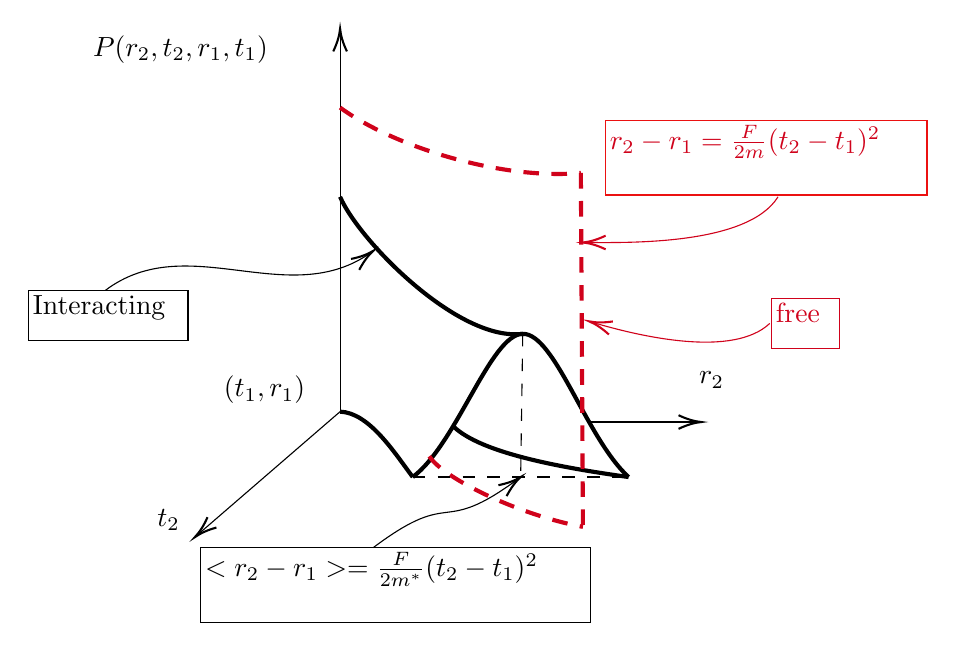
\begin{tikzpicture}[x=0.75pt,y=0.75pt,yscale=-1,xscale=1]
%uncomment if require: \path (0,300); %set diagram left start at 0, and has height of 300

%Curve Lines [id:da47195975974859194] 
\draw [line width=1.5]    (303.25,221.87) .. controls (324.47,205.95) and (340.75,153.06) .. (356.25,152.87) .. controls (371.75,152.67) and (386.71,203.02) .. (407.25,221.87) ;
%Curve Lines [id:da39634165547292277] 
\draw [line width=1.5]    (268.25,86.87) .. controls (277.25,107.87) and (325.25,156.87) .. (356.25,152.87) ;
%Straight Lines [id:da45989564554625706] 
\draw    (268.25,190.37) -- (268.25,7.87) ;
\draw [shift={(268.25,5.87)}, rotate = 450] [color={rgb, 255:red, 0; green, 0; blue, 0 }  ][line width=0.75]    (10.93,-3.29) .. controls (6.95,-1.4) and (3.31,-0.3) .. (0,0) .. controls (3.31,0.3) and (6.95,1.4) .. (10.93,3.29)   ;
%Straight Lines [id:da8675047275465586] 
\draw    (268.25,190.37) -- (199.76,249.56) ;
\draw [shift={(198.25,250.87)}, rotate = 319.15999999999997] [color={rgb, 255:red, 0; green, 0; blue, 0 }  ][line width=0.75]    (10.93,-3.29) .. controls (6.95,-1.4) and (3.31,-0.3) .. (0,0) .. controls (3.31,0.3) and (6.95,1.4) .. (10.93,3.29)   ;
%Straight Lines [id:da7098036303811813] 
\draw    (388.25,195.37) -- (440.25,195.37) ;
\draw [shift={(442.25,195.37)}, rotate = 180] [color={rgb, 255:red, 0; green, 0; blue, 0 }  ][line width=0.75]    (10.93,-3.29) .. controls (6.95,-1.4) and (3.31,-0.3) .. (0,0) .. controls (3.31,0.3) and (6.95,1.4) .. (10.93,3.29)   ;
%Curve Lines [id:da251060936963017] 
\draw [line width=1.5]    (268.25,190.37) .. controls (282.25,190.87) and (294.25,209.87) .. (303.25,221.87) ;
%Curve Lines [id:da7401245773765673] 
\draw [line width=1.5]    (323.25,197.87) .. controls (336.25,209.87) and (371.25,216.87) .. (407.25,221.87) ;
%Curve Lines [id:da4250361772641027] 
\draw [color={rgb, 255:red, 208; green, 2; blue, 27 }  ,draw opacity=1 ][line width=1.5]  [dash pattern={on 5.63pt off 4.5pt}]  (311.25,211.87) .. controls (318.25,222.87) and (355.25,240.37) .. (385.25,245.87) ;
%Straight Lines [id:da22876813296283727] 
\draw [color={rgb, 255:red, 208; green, 2; blue, 27 }  ,draw opacity=1 ][line width=1.5]  [dash pattern={on 5.63pt off 4.5pt}]  (384.25,75.37) -- (385.25,245.87) ;
%Curve Lines [id:da6869516606321976] 
\draw [color={rgb, 255:red, 208; green, 2; blue, 27 }  ,draw opacity=1 ][line width=1.5]  [dash pattern={on 5.63pt off 4.5pt}]  (268.25,43.87) .. controls (294.25,62.87) and (346.25,78.87) .. (384.25,75.37) ;
%Straight Lines [id:da7569475772419219] 
\draw  [dash pattern={on 4.5pt off 4.5pt}]  (356.25,152.87) -- (355.25,221.87) ;
%Straight Lines [id:da21545942112158833] 
\draw  [dash pattern={on 4.5pt off 4.5pt}]  (303.25,221.87) -- (407.25,221.87) ;
%Curve Lines [id:da6838743458498798] 
\draw    (284.25,255.87) .. controls (323.85,226.17) and (315.43,251.35) .. (354.06,222.75) ;
\draw [shift={(355.25,221.87)}, rotate = 503.13] [color={rgb, 255:red, 0; green, 0; blue, 0 }  ][line width=0.75]    (10.93,-3.29) .. controls (6.95,-1.4) and (3.31,-0.3) .. (0,0) .. controls (3.31,0.3) and (6.95,1.4) .. (10.93,3.29)   ;
%Curve Lines [id:da18599161011274368] 
\draw [color={rgb, 255:red, 208; green, 2; blue, 27 }  ,draw opacity=1 ]   (479.25,86.87) .. controls (464.7,110.15) and (407.81,108.96) .. (387.07,108.87) ;
\draw [shift={(385.25,108.87)}, rotate = 360] [color={rgb, 255:red, 208; green, 2; blue, 27 }  ,draw opacity=1 ][line width=0.75]    (10.93,-3.29) .. controls (6.95,-1.4) and (3.31,-0.3) .. (0,0) .. controls (3.31,0.3) and (6.95,1.4) .. (10.93,3.29)   ;
%Curve Lines [id:da8093943758486671] 
\draw    (155.25,131.87) .. controls (194.85,102.17) and (243.27,142.05) .. (283.05,113.75) ;
\draw [shift={(284.25,112.87)}, rotate = 503.13] [color={rgb, 255:red, 0; green, 0; blue, 0 }  ][line width=0.75]    (10.93,-3.29) .. controls (6.95,-1.4) and (3.31,-0.3) .. (0,0) .. controls (3.31,0.3) and (6.95,1.4) .. (10.93,3.29)   ;
%Curve Lines [id:da2739470314746484] 
\draw [color={rgb, 255:red, 208; green, 2; blue, 27 }  ,draw opacity=1 ]   (475.25,147.87) .. controls (457.7,164.44) and (413.53,154.4) .. (390.02,147.4) ;
\draw [shift={(388.25,146.87)}, rotate = 376.93] [color={rgb, 255:red, 208; green, 2; blue, 27 }  ,draw opacity=1 ][line width=0.75]    (10.93,-3.29) .. controls (6.95,-1.4) and (3.31,-0.3) .. (0,0) .. controls (3.31,0.3) and (6.95,1.4) .. (10.93,3.29)   ;

% Text Node
\draw (440,170) node [anchor=north west][inner sep=0.75pt]    {$r_{2}$};
% Text Node
\draw (179,236) node [anchor=north west][inner sep=0.75pt]    {$t_{2}$};
% Text Node
\draw (211,172) node [anchor=north west][inner sep=0.75pt]    {$( t_{1} ,r_{1})$};
% Text Node
\draw (148,8) node [anchor=north west][inner sep=0.75pt]    {$P( r_{2} ,t_{2} ,r_{1} ,t_{1})$};
% Text Node
\draw  [color={rgb, 255:red, 235; green, 17; blue, 17 }  ,draw opacity=1 ]  (396,50) -- (551,50) -- (551,86) -- (396,86) -- cycle  ;
\draw (397,51) node [anchor=north west][inner sep=0.75pt]  [color={rgb, 255:red, 208; green, 2; blue, 27 }  ,opacity=1 ]  {$r_{2} -r_{1} =\frac{F}{2m}( t_{2} -t_{1})^{2}$};
% Text Node
\draw    (201,256) -- (389,256) -- (389,292) -- (201,292) -- cycle  ;
\draw (202,257) node [anchor=north west][inner sep=0.75pt]    {$< r_{2} -r_{1}  >=\frac{F}{2m^*}( t_{2} -t_{1})^{2}$};
% Text Node
\draw    (118,132) -- (195,132) -- (195,156) -- (118,156) -- cycle  ;
\draw (119,133) node [anchor=north west][inner sep=0.75pt]   [align=left] {Interacting};
% Text Node
\draw  [color={rgb, 255:red, 208; green, 2; blue, 27 }  ,draw opacity=1 ]  (476,136) -- (509,136) -- (509,160) -- (476,160) -- cycle  ;
\draw (477,137) node [anchor=north west][inner sep=0.75pt]  [color={rgb, 255:red, 208; green, 2; blue, 27 }  ,opacity=1 ] [align=left] {free};


\end{tikzpicture}
    \caption{The classical propagator}
    \label{fig:classical-quasi-particle-example}
\end{figure}
If interactions between particles are now allowed to occur, this surface will \textbf{spread ou}t, as shown qualitatively. If we examine $\left\langle\mathbf{r}_{2}-\mathbf{r}_{1}\right\rangle,$ the position of the maximum value of $P$ in the interacting case, we see that for some types of interaction we might find that
\begin{equation}\left\langle\mathbf{r}_{2}-\mathbf{r}_{1}\right\rangle=\frac{1}{2}\left(\frac{\mathbf{F}}{m^{*}}\right)\left(t_{2}-t_{1}\right)^{2} \quad \text { for } P=\text { maximum }\end{equation}
If this is true, then \bluep{$\left\langle r_{2}-r_{1}\right\rangle$ behaves as the co-ordinate of a quasi particle of effective mass $m^{*} .$} Look now at the maximum height of $P$ as a function of $t_{2}$ Because of the 'spreading out' of the particle position, $P_{\max }$ will first fall infinitely rapidly from its value of $\infty$ at $t_{2}=t_{1},$ then more slowly. If this slower decay is exponential:
\begin{equation}P_{\max }\left(\mathbf{r}_{2}, t_{2}, \mathbf{r}_{1}, t_{1}\right) \propto e^{-\left(t_{2}-t_{1}\right) / \tau}\end{equation}
then \bluep{$\tau$ may be identified as the quasi particle lifetime;} it clearly must be fairly large if the quasi particle picture is to be useful. Thus, if we calculate $P$ and find that it shows the above behaviour, then the system is describable in terms of quasi particles and their lifetime and effective mass may be determined.

\subsection{Calculation of the Propagator by means of diagrams}
The actual calculation of the propagator P is quite complicated, but it is easy to illustrate all the principles involved with the aid of a simple analogue example in which the many-body system is replaced by \textbf{a set of fixed scattering centres}(e.g. A,B,C,D,E,F,G etc). A pinball is injected at the point $r_{1},$ at time $t_{1}$ and propagates through the system, being scattered at the various centres. We ask for the probability $P\left(\mathbf{r}_{2}, t_{2}, \mathbf{r}_{1}, t_{1}\right)$ that the particle reaches the point $r_{2}$ at time $t_{2}$.

The scattering mechanism is assumed to be such that (1) if the pinball strikes the scattering point $A$, then there is probability $P(A)$ that it is scattered and $1-P(A)$ that it will go straight through without scattering, (2) the probability distribution of pinball paths and velocities after scattering
at $A$ must be independent of the pinball path and velocity before scattering that is, the pinball loses its ' memory" of how it got to $A$.

For the sake of simplicity, let us leave time out of the argument to begin with, and consider just $P\left(\mathbf{r}_{2}, \mathbf{r}_{1}\right) ;$ this is the probability that if the particle begins at $r_{2}$ it will finish at $r_{2}$ regardless of the time. From the definition of probability, $P\left(\mathbf{r}_{2}, \mathbf{r}_{1}\right)$ is the sum of the probabilities for all the different ways the particle can go through which begin at $r_{1}$ and wind up at $r_{2}$. For example, the probability that the pinball will first hit scattering point $G$ and then end up at $r_2$ is:
\begin{equation}\left.P\left\{\left(\mathbf{r}_{1} \rightarrow \mathbf{r}_{G}\right), \text { (scattered at } \mathbf{r}_{G}\right),\left(\mathbf{r}_{G} \rightarrow \mathbf{r}_{2}\right)\right\}=P_{0}\left(\boldsymbol{r}_{G}, \mathbf{r}_{1}\right) P(G) P_{0}\left(\mathbf{r}_{2}, \mathbf{r}_{G}\right)\end{equation}
The total probability, $P\left(r_{2}, r_{1}\right),$ is just the sum of the probabilities for the various paths. Thus we find
\begin{equation}\begin{aligned}
&P\left(\mathbf{r}_{2}, \mathbf{r}_{1}\right)=P_{0}\left(\mathbf{r}_{2}, \mathbf{r}_{1}\right)+P_{0}\left(\mathbf{r}_{0}, \mathbf{r}_{1}\right) P(M) P_{0}\left(\mathbf{r}_{2}, \mathbf{r}_{0}\right)+P_{0}\left(\mathbf{r}_{M}, \mathbf{r}_{1}\right) P(M) P_{0}\left(\mathbf{r}_{2}, \mathbf{r}_{M}\right)+\\
&+P_{\mathrm{o}}\left(\mathbf{r}_{\boldsymbol{\sigma}}, \mathbf{r}_{1}\right) P(G) P_{\mathrm{o}}\left(\mathbf{r}_{\boldsymbol{G}}, \mathbf{r}_{\sigma}\right) P(G) P_{0}\left(\mathbf{r}_{2}, \mathbf{r}_{\sigma}\right)+\cdots
\end{aligned}\end{equation}
where M, and G are different scattering points.

How can this series be evaluated? If we assume that the $P_{0}$ 's are large, say $\sim \frac{1}{2}$ or so, and the various interaction $P(A)$ 's are small, say $\sim \frac{1}{10},$ then the higher order diagrams (i.e., \redp{note that by order here we mean the total number of interactions}) will give successively smaller contributions, and just as in ordinary perturbation theory, we can get an approximate solution by simply summing the series up through the first-or second-order terms. Thus, the zeroth-order approximation would be just the unperturbed case where the particle propagates freely from $\mathbf{r}_{1}$ to $\mathbf{r}_{2} .$ When we add the possibility of a perturbing (scattering) interaction with the various scattering points once each, we get the first-order approximation.

Allowing two interactions gives the second-order approximation and so on. \bluep{If, on the other hand, one or more of the interaction terms $P(A)$ is large (i.e., strong scattering at $A$ ) this method is not practical, since the series converges too slowly, and the summation must be carried out to extremely high orders to give a good result.}

However, there is another kind of approximation where we do not stop at low order interactions, but instead sums over important diagrams to infinite order. Suppose for example, that only $P(M)$ is large and all the other $P(X)$ are small. Then the "M" diagrams will dominate, and the series may be approximated by the sum over just repeated "M"s, thus:
\begin{center}
\tikzset{every picture/.style={line width=0.75pt}} %set default line width to 0.75pt        

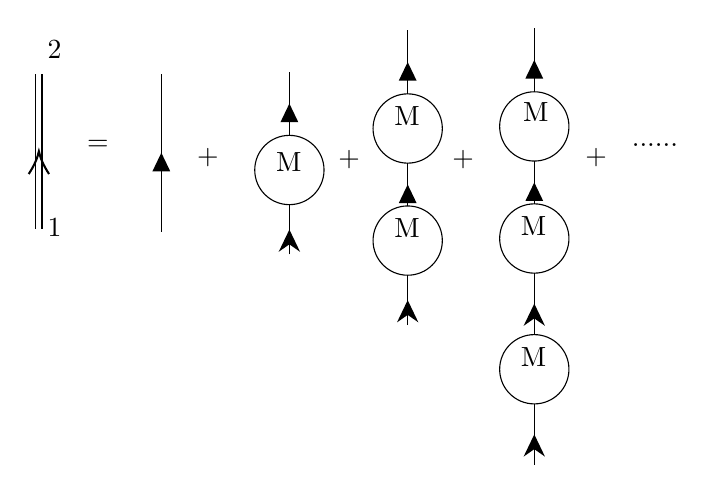
\begin{tikzpicture}[x=0.75pt,y=0.75pt,yscale=-1,xscale=1]
%uncomment if require: \path (0,349); %set diagram left start at 0, and has height of 349

%Straight Lines [id:da4757935872975344] 
\draw    (8.07,101.32) -- (8.07,26.7)(11.07,101.32) -- (11.07,26.7) ;
\draw [shift={(9.57,64.01)}, rotate = 450] [color={rgb, 255:red, 0; green, 0; blue, 0 }  ][line width=0.75]    (10.93,-4.9) .. controls (6.95,-2.3) and (3.31,-0.67) .. (0,0) .. controls (3.31,0.67) and (6.95,2.3) .. (10.93,4.9)   ;
%Straight Lines [id:da23622371172830803] 
\draw    (68.57,102.7) -- (68.57,26.7) ;
\draw [shift={(68.57,64.7)}, rotate = 450] [fill={rgb, 255:red, 0; green, 0; blue, 0 }  ][line width=0.08]  [draw opacity=0] (8.93,-4.29) -- (0,0) -- (8.93,4.29) -- cycle    ;
%Shape: Circle [id:dp4139523862436749] 
\draw   (113.57,73.01) .. controls (113.57,63.79) and (121.04,56.32) .. (130.26,56.32) .. controls (139.48,56.32) and (146.95,63.79) .. (146.95,73.01) .. controls (146.95,82.23) and (139.48,89.7) .. (130.26,89.7) .. controls (121.04,89.7) and (113.57,82.23) .. (113.57,73.01) -- cycle ;
%Straight Lines [id:da33169967910609544] 
\draw    (130.26,56.32) -- (130.26,25.7) ;
\draw [shift={(130.26,41.01)}, rotate = 450] [fill={rgb, 255:red, 0; green, 0; blue, 0 }  ][line width=0.08]  [draw opacity=0] (8.93,-4.29) -- (0,0) -- (8.93,4.29) -- cycle    ;
%Straight Lines [id:da28347419222198567] 
\draw    (130.26,113.7) -- (130.26,89.7) ;
\draw [shift={(130.26,101.7)}, rotate = 450] [fill={rgb, 255:red, 0; green, 0; blue, 0 }  ][line width=0.08]  [draw opacity=0] (10.72,-5.15) -- (0,0) -- (10.72,5.15) -- (7.12,0) -- cycle    ;
%Shape: Circle [id:dp663325870350397] 
\draw   (170.57,107.01) .. controls (170.57,97.79) and (178.04,90.32) .. (187.26,90.32) .. controls (196.48,90.32) and (203.95,97.79) .. (203.95,107.01) .. controls (203.95,116.23) and (196.48,123.7) .. (187.26,123.7) .. controls (178.04,123.7) and (170.57,116.23) .. (170.57,107.01) -- cycle ;
%Straight Lines [id:da6913773132395338] 
\draw    (187.26,36.32) -- (187.26,5.7) ;
\draw [shift={(187.26,21.01)}, rotate = 450] [fill={rgb, 255:red, 0; green, 0; blue, 0 }  ][line width=0.08]  [draw opacity=0] (8.93,-4.29) -- (0,0) -- (8.93,4.29) -- cycle    ;
%Straight Lines [id:da4724377841227787] 
\draw    (187.26,147.7) -- (187.26,123.7) ;
\draw [shift={(187.26,135.7)}, rotate = 450] [fill={rgb, 255:red, 0; green, 0; blue, 0 }  ][line width=0.08]  [draw opacity=0] (10.72,-5.15) -- (0,0) -- (10.72,5.15) -- (7.12,0) -- cycle    ;
%Shape: Circle [id:dp29262051024858293] 
\draw   (170.57,53.01) .. controls (170.57,43.79) and (178.04,36.32) .. (187.26,36.32) .. controls (196.48,36.32) and (203.95,43.79) .. (203.95,53.01) .. controls (203.95,62.23) and (196.48,69.7) .. (187.26,69.7) .. controls (178.04,69.7) and (170.57,62.23) .. (170.57,53.01) -- cycle ;
%Straight Lines [id:da2293551017015375] 
\draw    (187.26,69.7) -- (187.26,90.32) ;
\draw [shift={(187.26,80.01)}, rotate = 90] [fill={rgb, 255:red, 0; green, 0; blue, 0 }  ][line width=0.08]  [draw opacity=0] (8.93,-4.29) -- (0,0) -- (8.93,4.29) -- cycle    ;
%Shape: Circle [id:dp5742274191772756] 
\draw   (231.57,106.01) .. controls (231.57,96.79) and (239.04,89.32) .. (248.26,89.32) .. controls (257.48,89.32) and (264.95,96.79) .. (264.95,106.01) .. controls (264.95,115.23) and (257.48,122.7) .. (248.26,122.7) .. controls (239.04,122.7) and (231.57,115.23) .. (231.57,106.01) -- cycle ;
%Straight Lines [id:da8337372469854066] 
\draw    (248.26,35.32) -- (248.26,4.7) ;
\draw [shift={(248.26,20.01)}, rotate = 450] [fill={rgb, 255:red, 0; green, 0; blue, 0 }  ][line width=0.08]  [draw opacity=0] (8.93,-4.29) -- (0,0) -- (8.93,4.29) -- cycle    ;
%Straight Lines [id:da42712440571211296] 
\draw    (248.26,152.07) -- (248.26,122.7) ;
\draw [shift={(248.26,137.38)}, rotate = 450] [fill={rgb, 255:red, 0; green, 0; blue, 0 }  ][line width=0.08]  [draw opacity=0] (10.72,-5.15) -- (0,0) -- (10.72,5.15) -- (7.12,0) -- cycle    ;
%Shape: Circle [id:dp5287893719741432] 
\draw   (231.57,52.01) .. controls (231.57,42.79) and (239.04,35.32) .. (248.26,35.32) .. controls (257.48,35.32) and (264.95,42.79) .. (264.95,52.01) .. controls (264.95,61.23) and (257.48,68.7) .. (248.26,68.7) .. controls (239.04,68.7) and (231.57,61.23) .. (231.57,52.01) -- cycle ;
%Straight Lines [id:da8377025286119076] 
\draw    (248.26,68.7) -- (248.26,89.32) ;
\draw [shift={(248.26,79.01)}, rotate = 90] [fill={rgb, 255:red, 0; green, 0; blue, 0 }  ][line width=0.08]  [draw opacity=0] (8.93,-4.29) -- (0,0) -- (8.93,4.29) -- cycle    ;
%Shape: Circle [id:dp8985140189745163] 
\draw   (231.57,169.01) .. controls (231.57,159.79) and (239.04,152.32) .. (248.26,152.32) .. controls (257.48,152.32) and (264.95,159.79) .. (264.95,169.01) .. controls (264.95,178.23) and (257.48,185.7) .. (248.26,185.7) .. controls (239.04,185.7) and (231.57,178.23) .. (231.57,169.01) -- cycle ;
%Straight Lines [id:da5985992460409527] 
\draw    (248.26,215.07) -- (248.26,185.7) ;
\draw [shift={(248.26,200.38)}, rotate = 450] [fill={rgb, 255:red, 0; green, 0; blue, 0 }  ][line width=0.08]  [draw opacity=0] (10.72,-5.15) -- (0,0) -- (10.72,5.15) -- (7.12,0) -- cycle    ;

% Text Node
\draw (12.57,95.32) node [anchor=north west][inner sep=0.75pt]   [align=left] {1};
% Text Node
\draw (12.57,9.32) node [anchor=north west][inner sep=0.75pt]   [align=left] {2};
% Text Node
\draw (31.57,57.32) node [anchor=north west][inner sep=0.75pt]   [align=left] {=};
% Text Node
\draw (122.57,63.32) node [anchor=north west][inner sep=0.75pt]   [align=left] {M};
% Text Node
\draw (241.57,39.32) node [anchor=north west][inner sep=0.75pt]   [align=left] {M};
% Text Node
\draw (240.57,94.32) node [anchor=north west][inner sep=0.75pt]   [align=left] {M};
% Text Node
\draw (179.57,95.32) node [anchor=north west][inner sep=0.75pt]   [align=left] {M};
% Text Node
\draw (179.57,41.32) node [anchor=north west][inner sep=0.75pt]   [align=left] {M};
% Text Node
\draw (84.57,61.32) node [anchor=north west][inner sep=0.75pt]    {$+$};
% Text Node
\draw (152.57,62.32) node [anchor=north west][inner sep=0.75pt]    {$+$};
% Text Node
\draw (207.57,62.32) node [anchor=north west][inner sep=0.75pt]    {$+$};
% Text Node
\draw (271.57,61.32) node [anchor=north west][inner sep=0.75pt]    {$+$};
% Text Node
\draw (240.57,157.32) node [anchor=north west][inner sep=0.75pt]   [align=left] {M};
% Text Node
\draw (294,59) node [anchor=north west][inner sep=0.75pt]   [align=left] {......};


\end{tikzpicture}

\end{center}
Translating each element of the diagrams into the appropriate probability, it is easy to write down the corresponding series:
$$\begin{aligned}
P\left(\mathbf{r}_{2}, \mathbf{r}_{1}\right) \approx P_{0} &\left(\mathbf{r}_{2}, \mathbf{r}_{1}\right)+P_{0}\left(\mathbf{r}_{\mathbf{M}}, \mathbf{r}_{1}\right) P(M) P_{0}\left(\mathbf{r}_{2}, \mathbf{r}_{M}\right)+\\
&+P_{0}\left(\mathbf{r}_{M}, \mathbf{r}_{1}\right) P(M) P_{0}\left(\mathbf{r}_{M}, \mathbf{r}_{M}\right) P(M) P_{0}\left(\mathbf{r}_{2}, \mathbf{r}_{M}\right)+\cdots
\end{aligned}$$
and
$$\begin{aligned}
P\left(\mathbf{r}_{2}, \mathbf{r}_{1}\right) \approx P_{0}\left(\mathbf{r}_{2}, \mathbf{r}_{1}\right)+P_{0}\left(\mathbf{r}_{M}, \mathbf{r}_{1}\right) P(M) P_{0}\left(\mathbf{r}_{2}, \mathbf{r}_{M}\right) \times & \\
\times\left[1+P(M) P_{0}\left(\mathbf{r}_{M}, \mathbf{r}_{M}\right)+P(M)^{2} P_{0}\left(\mathbf{r}_{M}, \mathbf{r}_{M}\right)^{2}+\cdots\right] \\
=P_{0}\left(\mathbf{r}_{2}, \mathbf{r}_{1}\right)+\frac{P_{0}\left(\mathbf{r}_{M}, \mathbf{r}_{1}\right) P(M) P_{0}\left(\mathbf{r}_{2}, \mathbf{r}_{M}\right)}{1-P(M) P_{0}\left(\mathbf{r}_{M}, \mathbf{r}_{M}\right)}
\end{aligned}$$
This new approximation, involving the summation of a perturbation series to infinite order over a selected class of repeated diagrams (i.e., terms) is called' partial summation' or' selective summation'. It is drastically different from the ordinary perturbation approximation.

The above diagram technique may easily be extended to the time-dependent propagator, $P\left(\mathbf{r}_{2}, \mathbf{r}_{1}, t_{2}-t_{1}\right) .$ (We have written $t_{2}-t_{1}$ since the force is time independent so the propagators can depend only on time differences.) Let $P_{0}\left(\mathbf{r}_{j}, \mathbf{r}_{i}, t_{j}-t_{i}\right)=$ probability that if the particle leaves the point $\mathbf{r}_{i}$ at time $t_{i}$ then it arrives at $r_{j}$ at time $t_{j}$ without undergoing any interaction on the way (this is the 'free propagator'). Let $P(A)$ be the interaction term, assumed instantaneous for simplicity. Then, we have
\begin{equation}\begin{aligned}
P\left(\mathbf{r}_{2}, \mathbf{r}_{1}, t_{2}-t_{1}\right)=& P_{0}\left(\mathbf{r}_{2}, \mathbf{r}_{1}, t_{2}-t_{1}\right)+\\
&+\int_{t_{1}}^{t_{2}} d t_{G} P_{0}\left(\mathbf{r}_{G}, \mathbf{r}_{1}, t_{G}-t_{1}\right) P(G) P_{0}\left(\mathbf{r}_{2}, \mathbf{r}_{G}, t_{2}-t_{G}\right)+\\
&+\int d t_{M} \cdots+\iint+\cdots+\iiint+\cdots+\cdots
\end{aligned}
\label{pinball-example}
\end{equation}
The integrals parading through this expansion can be removed by noticing that they all have the form of "folded" products. This means they can be converted into simple products by a Fourier transformation. Suppose we define the transformed propagator, $P_0(\mathbf{r}_j,\mathbf{r}_i,\omega)$ by
\begin{equation}P_{0}\left(\mathbf{r}_{j}, \mathbf{r}_{i}, t_{j}-t_{l}\right)=\frac{1}{2 \pi} \int_{-\infty}^{+\infty} d \omega e^{-i \omega\left(t_{j}-t_i\right)} P_{0}\left(\mathbf{r}_{j}, \mathbf{r}_{i}, \omega\right)\end{equation}
with a similar expression for $P\left(\mathbf{r}_{j}, \mathbf{r}_{l}, \omega\right) .$ Then the first two terms of (\ref{pinball-example}) become (note that we can integrate over $t_{G}$ from $-\infty$ to $+\infty$ because condition
(\ref{zero-condition}) automatically limits the integral to the region $t_{1} \rightarrow t_{2}$ ):
$$P_{0}\left(\mathbf{r}_{2}, \mathbf{r}_{1}, t_{2}-t_{1}\right)=\frac{1}{2 \pi} \int_{-\infty}^{+\infty} d \omega e^{-i \omega\left(t_{2}-t_{1}\right)} P_{0}\left(\mathbf{r}_{2}, \mathbf{r}_{1}, \omega\right)$$
$$\begin{array}{l}
\int_{-\infty}^{+\infty} d t_{G} P_{0}\left(\mathbf{r}_{G}, \mathbf{r}_{1}, t_{G}-t_{1}\right) P(G) P_{0}\left(\mathbf{r}_{2}, \mathbf{r}_{G}, t_{2}-t_{G}\right)= \\
=\int_{-\infty}^{+\infty} d t_{G}\left[\frac{1}{2 \pi} \int_{-\infty}^{+\infty} d \omega^{\prime} e^{-i \omega^{\prime}\left(t_{G}-t\right)} P_{0}\left(\mathbf{r}_{G}, \mathbf{r}_{1}, \omega^{\prime}\right)\right] \times \\
\quad \times P(G) \times\left[\frac{1}{2 \pi} \int_{-\infty}^{+\infty} d \omega e^{-i \omega\left(t_{2}-t_{G}\right)} P_{0}\left(\mathbf{r}_{2}, \mathbf{r}_{G}, \omega\right)\right]=
\end{array}$$
$$\begin{array}{c}
=\frac{1}{(2 \pi)^{2}} \int_{-\infty}^{+\infty} d \omega \int_{-\infty}^{+\infty} d \omega^{\prime} P_{0}\left(\mathbf{r}_{G}, \mathbf{r}_{1}, \omega^{\prime}\right) \times \\
\times P(G) P_{0}\left(\mathbf{r}_{2}, \mathbf{r}_{G}, \omega\right) e^{+i\left(\omega^{\prime} t_{1}-\omega t_{2}\right)} \int_{-\infty}^{+\infty} d t_{G} e^{-i t_{0}\left(\omega^{\prime}-\omega\right)}
\end{array}$$
Since
\begin{imp}
\begin{equation}
2 \pi \delta\left(\omega^{\prime}-\omega\right)=\int_{-\infty}^{+\infty} d t_{G} e^{-i t_{G}\left(\omega^{\prime}-\omega\right)}\end{equation}
\end{imp}
we have
\begin{equation}
\begin{aligned}
\int_{-\infty}^{+\infty} d t_{G} P_{0}\left(\mathbf{r}_{G}, \mathbf{r}_{1}, t_{G}-t_{1}\right) P(G) P_{0}\left(\mathbf{r}_{2}, \mathbf{r}_{G}, t_{2}-t_{G}\right)&=\\
&\frac{1}{2 \pi} \int_{-\infty}^{+\infty} d \omega e^{-i \omega\left(t_{2}-t_{1}\right)} P_{0}\left(\mathbf{r}_{G}, \mathbf{r}_{1}, \omega\right) P(G) P_{0}\left(\mathbf{r}_{2}, \mathbf{r}_{G}, \omega\right)
\end{aligned}
\end{equation}
Continuing thus, and finally taking the inverse transform, yields
\begin{equation}P\left(\mathbf{r}_{2}, \mathbf{r}_{1}, \omega\right)=P_{0}\left(\mathbf{r}_{2}, \mathbf{r}_{1}, \omega\right)+P_{0}\left(\mathbf{r}_{G}, \mathbf{r}_{1}, \omega\right) P(G) P_{0}\left(\mathbf{r}_{2}, \mathbf{r}_{G}, \omega\right)+\cdots\end{equation}

\newpage
\section{Quantum Quasi Particles and the Quantum Pinball Propagator}
In the quantum case, the total probability amplitude is the sum of the probability amplitudes for each process taken separately
$$G(2,1)=G(\text { process } 1)+G(\text { process } 11)+\cdots$$
so that the corresponding probability is given by
$$P(2,1)_{\text {quantum }}=G^{*} G=\underbrace{|G(\mathrm{I})|^{2}}_{P(\mathrm{I})}+\underbrace{|G(\mathrm{I})|^{2}}_{P(\mathrm{II})}+\underbrace{G(\mathrm{I})^{*} G(\mathrm{II})+G(\mathrm{II})^{*} G(\mathrm{I})}_{\text {interference terms }}+\cdots$$
Because of the characteristic interference terms', the quantum probability is not just the sum of the probabilities for the individual processes, in contrast to the classical case.

Let us begin by defining the quantum propagator in general, then show
what it looks like in the case of free particles and quasi particles. The quantum analogue of the classical propagator is (assuming that the Hamiltonian is time-independent, so that the propagator depends only on time differences):
\begin{imp}
\begin{equation}i G\left(\mathrm{r}_{2}, \mathrm{r}_{1}, t_{2}-t_{1}\right)_{t_{2}>t_{1}}=i G^{+}\left(\mathrm{x}_{2}, \mathrm{r}_{1}, t_{2}-t_{1}\right)\end{equation}
probability amplitude that if at time $t_{1}$ we add a particle at point $r_{1}$ to the interacting system in its ground state, then at time $t_{2}$ the system will be in its ground state with an added particle at $\mathbf{r}_{2}$
\end{imp}
The $i$ factor is purely for decoration (a matter of convention) and the $+$ superscript denotes $t_{2}>t_{1} .$ The probability corresponding to the amplitude is
$$P\left(\mathbf{r}_{2}, \mathbf{r}_{1}, t_{2}-t_{1}\right)=G^{+}\left(r_{2}, \mathbf{r}_{1}, t_{2}-t_{1}\right)^{*} G^{+}\left(\mathbf{r}_{2}, \mathbf{r}_{1}, t_{2}-t_{1}\right)$$
Note that it is not necessarily the 'same' particle which is observed at 12, since
this has no meaning in the systems of identical particles with which we shall generally deal. The quantity $G^{+}$ is called a \bluep{'retarded' propagator (or Green's function)}. By definition, it is equal to zero for $t_{2} \leqslant t_{1} .$ There is also an \bluep{'advanced' propagator, $G^{-},$ which is finite for $t_{2} \leqslant t_{1} $}.

It is actually more convenient to work with an equivalent definition of $G$ in terms of arbitrary single-particle eigenstates, $\phi_{k}(r),$ instead of position eigenstates. Then we have \redp{$i G^{+}\left(k_{2}, k_{1}, t_{2}-t_{1}\right)_{t_{2}>t_{1}}=$probability amplitude that if at time $t_{1}$ we add a particle in $\phi_{k_{1}}(r)$ to the interacting system in its ground state, then at time $t_{2}$ the system will be in its ground state with an added particle in $\phi_{k_{2}}(r)$}.
For $t_{2} \leqslant t_{1}, G^{+}$ is defined so that:
\begin{equation}i G^{+}\left(k_{2}, k_{1}, t_{2}-t_{1}\right)_{t_{2}\leq t_{1}}=0\end{equation}
\textbf{A convenient choice for $\phi_{k}(r)$ is the eigenstates of the unperturbed single particle Hamiltonian, which we will call $H_{0}$ :}
$$H_{0}=\frac{p^{2}}{2 m}+U(\mathrm{r})=-\frac{1}{2 m} \nabla_{r}^{2}+U(\mathrm{r}) \quad(\hbar=1)$$
If $U(\mathrm{r})=0,$ then this is just the free particle case:
$$H_{0} \phi_{k}(\mathbf{r})=\epsilon_{k} \phi_{k}(\mathbf{r})$$
and
\begin{equation}H_{0}=-\frac{\nabla_{r}^{2}}{2 m}, \quad \phi_{k}(r)=\frac{1}{\sqrt{\Omega}} e^{i k \cdot r}, \quad \epsilon_{k}=\frac{k^{2}}{2 m}
\label{nrqm-free-particle}
\end{equation}
where $\Omega$ is normalization volume and spin is neglected for simplicity. Note that if $k_1=k_2$, the particle propagates in time only.

Let us first get the free propagator $G_{0}^{+}$ (no perturbing interaction). Suppose at time $t_{1}$ the wave function of the free particle is $\phi_{k,}(\mathrm{r}) .$ Then we have:
$$\psi\left(\mathbf{r}, t_{1}\right)=\phi_{\mathbf{k}_{2}}(\mathbf{r})$$
At later time $t_{2},$ by the time-dependent Schrödinger equation, we find that the wave function has become
\begin{equation}\psi\left(\mathbf{r}, t_{2}\right)=\phi_{k_{1}}(\mathbf{r}) e^{-i \varepsilon_{k1}\left(t_{2}-t_{1}\right)}
\end{equation}
where $\epsilon_{k_{1}}$ is the single particle energy of undisturbed Shrodinger equation. The probability amplitude for the particle being in state $\phi_{k_{2}}$ at time $t_{2}$ is /hen just the component of $\psi\left(\mathbf{r}, t_{2}\right)$ along $\phi_{k_{2}}$ or:
\begin{equation}\int d^{3} \mathbf{r} \psi\left(\mathbf{r}, t_{2}\right) \phi_{k_{2}}^{*}(\mathbf{r})=e^{-i \exp \left(l_{2}-t_{1}\right)} \int \underbrace{d^{3} \mathbf{r} \phi_{k_{1}}(\mathbf{r}) \phi_{k_{2}}^{*}(\mathbf{r})}_{\delta_{k_{2} k_{1}}}\end{equation}
whence, by definition
\begin{equation}G_{0}^{+}\left(k, t_{2}-t_{1}\right)=\left\{\begin{array}{ll}
-i \theta_{12-t_{1}} e^{-i \epsilon_{k_1}\left(t_{2}-t_{1}\right)}, & \text { for } t_{2} \neq t_{1} \\
0, & \text { for } t_{2}=t_{1}
\end{array}\right.
\label{G0-+}
\end{equation}
where
$$\theta_{t_{2}-t_{1}}\left\{\begin{array}{ll}
=1, & \text { if } t_{2}>t_{1} \\
=0, & \text { if } t_{2}<t_{1}
\end{array}\right.$$
\bluep{Note that for fermions, all levles up to $\epsilon_F$(=Fermi energy) are fileed, so we can only propagate a particle with $\epsilon_{k_1}>\epsilon_F$}. The Fourier transform of (\ref{G0-+}) is
\begin{equation}\begin{aligned}
G_{0}^{+}(k, \omega) &=-i \int_{-\infty}^{+\infty} d\left(t_{2}-t_{1}\right) \theta_{t_{2}-t_{1}} e^{i \omega\left(t_{2}-t_{1}\right)} e^{-i \epsilon_{k}\left(t_{2}-t_{1}\right)} \\
&=\left.(-1) \frac{e^{i\left(\omega-\epsilon_{k}\right)\left(t_{2}-t_{1}\right)}}{\omega-\epsilon_{k}}\right|_{0} ^{\infty}=\frac{1}{\omega-\epsilon_{k}}-\frac{e^{i\left(\omega-\epsilon_{k}\right)\infty}}{\omega-\epsilon_{k}}
\end{aligned}
\label{G0-k-omega}
\end{equation}
\redp{Because of the exponential oscillating at $\infty,$ this function is not well defined. In order to get around this difficulty, we have to slightly modify the expression for the free propagator. This is done by multiplying the propagator by the factor $\exp \left(-\delta\left(t_{2}-t_{1}\right)\right),$ where $\delta$ is a positive infinitesimal such that $\delta \times \infty=\infty$}. Then (\ref{G0-+}) becomes:
\begin{equation}G_{0}^{+}\left(k, t_{2}-t_{1}\right)=-i \theta_{t_{2}-t_{1}}e^{i(\epsilon_k-i\delta)(t_2-t_1)}
\label{G0-with-delta}
\end{equation}
For any finite $\left(t_{2}-t_{1}\right),$ we have $\delta \times\left(t_{2}-t_{1}\right)=0,$ so this is just $(3.10) .$ But for infinite $\left(t_{2}-t_{1}\right), \delta \times\left(t_{2}-t_{1}\right)=\infty$ so $G_{0}^{+}=0 .$ When \ref{G0-with-delta} is placed in \ref{G0-k-omega} we find
\begin{imp}
\begin{equation}G_{o}^{+}(k, \omega)=\frac{1}{\omega-\epsilon_{k}+i \delta}
\label{G0-k-omega-delta}
\end{equation}
\end{imp}
\bluep{From \ref{G0-k-omega-delta} we see the pole is at $\omega=\epsilon_k$, the eigenvalue for the eigenstate $\phi_k$. It turns out this observation is quite general, even for interacting propagator, $G^0(k,l;\omega)$:}
\begin{imp}
The poles of $G^+(k,l,\omega),$ the fourier transform of the single-particle propagator, corresponds to the excited energy of (N+1)-particle system \textbf{minus the ground state energy of N-particle system}.
\end{imp}
Also from \ref{G0-k-omega-delta}, we have the particle lifetime $\tau$ as $\delta^{-1}=\infty$, which makes sense because we only consider one free particle here. This observation can also be extended to interacting system where the propagator has the form of 
\begin{equation}
    G^+=\frac{1}{\omega-\epsilon_k^{\prime}+i\tau_k^{-1}}
\end{equation}
where \redp{$\tau_k$ is the quasi-particle lifetime at the state of $\epsilon_k$}.

In a Fermi system, because of the Pauli's principle, each state can only be occupied by one fermion. If a state is partially occupied by a fermion, the possibility of adding another fermion at the same state will be less than 1. Hence we have to multiply the propagator by a factor $Z_k\leq 1$:
\begin{equation}G_{\text {\stackanchor{quasi}{particle} }}^{+}\left(k,t_{2}-t_{1}\right)=-i Z_{k} e^{-i \epsilon_{k}^{\prime}\left(t_{2}-t_{1}\right)} e^{-\left(t_{2}-t_{1}\right) / \tau_{k}}\end{equation}
\begin{equation}G_{\text {\stackanchor{quasi}{particle}}}^{+}(k, \omega)=\frac{Z_{k}}{\omega-\epsilon_{k}^{\prime}+i \tau_{k}^{-1}}\end{equation}
The poles in the equation above are 
\begin{equation}
    \omega = \epsilon_k^{\prime}-i\tau_k^{-1}
\end{equation}
We can still interpret these poles as the excited energy levels even though they are imaginary numbers. For free particles, we have eigenstates as:
$$
\psi_k(x)=\phi_k(x)e^{-i\epsilon_k t}
$$
When the weak interaction is turned on, the particle decays out of state "$k$", we have
$$
\psi_k(x)\approx\phi_k(x)e^{-i\epsilon_k^{\prime} t}e^{-t/\tau_k}=\phi_k(x)e^{-i(\epsilon_k^{\prime}-i\tau^{-1})t}
$$

\subsection{Quantum Pinball Game}
Like the classical pinball game, we now consider the quantum version of the game where \redp{the "scattering centers" are now "scattering fields/potentials"}. Let's assume that a perturbative potential that interacts with free particle has a form of:
\begin{equation}V(\mathbf{p})=V_{M}+V_{L}=M p^{2}+L p^{4}=-M \nabla_{r}^{2}+L \nabla_{r}^{4}\end{equation}
where $M \geqslant L$. By solving the Schrodinger equation we have the Hamiltonian as
$$
H = (\frac{1}{2m}+M+Lp^2)p^2
$$
with 
$$
\epsilon_k^{\prime}= (\frac{1}{2m}+M+Lk^2)k^2
$$
and $\phi_k(x)=\frac{1}{\sqrt{\Omega}}e^{-i\mathbf{k}\cdot\mathbf{r}}$.\bluep{Now let us solve for the eigenvalues in a propagator way.}

The simplest way the particle can propagate through the system is without interaction, which has a propability amplitude as $G^+(k,t_2-t_1)$. Another way is to enter in $\phi_{k_{1}}$ at time $t_{1},$ be scattered into state $\phi_{k_{2}}$ at time $t_{M}$ by the potential $V_{M},$ then continue freely in $\phi_{k_{2}}$ until time $t_{2} .$ The probability amplitude in this case is just the product of the probability amplitude for each independent process:
$$
G^+_0(k_1,t_M-t_1)V_MG^+_0(k_1,t_2-t_M)
$$
$V_M$ can be obtained from time-dependent perturbation theory as follows: Let $c_{l}$ be the probability amplitude that at time $t_{0}$ a system is in state $\phi_{l} .$ Then at later time, $t,$ the time rate of change of any particular $c_{l},$ say $c_{p},$ under the influence of perturbation $V$, is given by:
\begin{equation}\dot{c}_{p}(t)=-i \sum_{l} V_{p l} c_{l} e^{i\left(\epsilon_{p}-c_{l}\right)\left(t-t_{o}\right)}\end{equation}
where $V_{pl}$ is just the element of S matrix. Hence the probability amplitude per unit time that the system undergoes a transition from $\phi_{k_1}$ to $\phi_p=\phi_{k_2}$, at time $t_M$ is:
\begin{equation}\begin{aligned}
\dot{c}_{k_{2}}\left(t=t_{M}\right) &=-i V_{M_{k_2 k_1}}=-i \int d^{3} \mathbf{r} \phi_{k_{2}}^{*}(r) V_{M} \phi_{k_{1}}(r)=\\
&=+i M \int d^{3} \mathbf{r} \phi_{k_{2}}^{*} \nabla^{2} \phi_{k_{1}}=-i M k_{1}^{2} \delta_{k_{2} k_{1}}
\end{aligned}\end{equation}
Thus the probability amplitude for this first-order scattering is 
\begin{equation}
    \left[\text{\stackanchor{probability}{amplitude}}\right]_{t_1\rightarrow t_M\rightarrow t_2}=i \int_{-\infty}^{+\infty} d t_{M} G_{0}^{+}\left(\mathbf{k}_{1}, t_{M}-t_{1}\right) V_{M_{k_2k_1}} G_{0}^{+}\left(\mathbf{k}_{2}, t_{2}-t_{M}\right)
\end{equation}
Similarly for $V_L$, we have
$$-i V_{L_{k_1k_2}}=-i L k_{1}^{4} \delta_{k_{2} k_{1}}$$
which also conserves momentum. There are also second- and higher-order processes in which the particle collides with $V_{M}$ and $V_{L}$ any number of times. This gives us the series expansion for the propagator (set $\mathbf{k}_{1}=\mathbf{k}_{2}=\mathbf{k}$ because of conservation of momentum here), after cancelling the $i$ 's:
$$\begin{aligned}
G^{+}\left(\mathbf{k}, t_{2}-t_{1}\right)=G_{0}^{+} &\left(\mathbf{k}, t_{2}-t_{1}\right)+\int_{-\infty}^{+\infty} d t_{M} G_{0}^{+}\left(\mathbf{k}, t_{M}-t_{1}\right) V_{M} G_{0}^{+}\left(\mathbf{k}, t_{2}-t_{M}\right) \\
&+\int_{-\infty}^{+\infty} d t_{L} G_{0}^{+}\left(\mathbf{k}, t_{L}-t_{1}\right) V_{L} G_{0}^{+}\left(\mathbf{k}, t_{2}-t_{L}\right)+\\
&+\int d t_{M} d t_{M}^{\prime} \cdots+\int d t_{M} d t_{L} \cdots+\cdots
\end{aligned}$$
Taking the Fourier transform, we have
\begin{equation}\begin{aligned}
G^{+}(\mathbf{k}, \omega)=G_{0}^{+} &(\mathbf{k}, \omega)+\left[G_{0}^{+}(\mathbf{k}, \omega)\right]^{2} V_{M_{k k}}+\left[G_{0}^{+}(\mathbf{k}, \omega)\right]^{2} V_{L_{kk}}+\\
&+\left[G_{0}^{+}\right]^{3} V_{M_{kk}}^{2}+2\left[G_{0}^{+}\right]^{3} V_{M_{kk}} V_{L_{kk}}+\left[G_{0}^{+}\right]^{3} V_{L_{kk}}^{2}+\\
&+\left[G_{0}^{+}\right]^{4} V_{M_{kk}}^{3}+\cdots
\end{aligned}\end{equation}
We now pull the trick of \redp{partial summation} here. We assume that the scattering with $V_M$ is much more important than the scattering with $V_L$, then the Feynman diagram series can be approximated by:

\newpage
\section{Quantum Particle in Fermi System}
\subsection{Propagator method in many-body systems}
In this chapter we will start with non-interacting Fermi-system problem. This is really a fake many-body problem,since as the problem is actually only a one-body problem. By doing this trivial problem, we will describe Fermi system very simply in terms of a few particles above the Fermi level, and a few removed particles, or "holes" below. Second, it allows us to introduce the language of the many-body problem,"\bluep{occupation number formalism}", or "\bluep{second quantization}". Finally, it shows us how to extend the definition of the propagator to the case where $t_2<t_1$. In this case, \textbf{the Green's function turns out to describe the propagation of removed particles, or "holes", which are represented diagrammatically by a downward-going arrow.}

By introducing a tree-level two-body interaction 
\begin{center}
\tikzset{every picture/.style={line width=0.75pt}} %set default line width to 0.75pt        

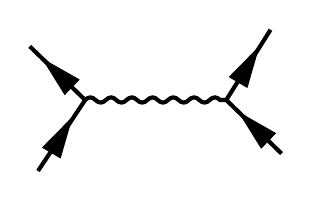
\begin{tikzpicture}[x=0.75pt,y=0.75pt,yscale=-1,xscale=1]
%uncomment if require: \path (0,705); %set diagram left start at 0, and has height of 705

%Straight Lines [id:da613823184290475] 
\draw [line width=1.5]    (491.42,548.13) .. controls (493.09,546.46) and (494.75,546.46) .. (496.42,548.13) .. controls (498.09,549.8) and (499.75,549.8) .. (501.42,548.13) .. controls (503.09,546.46) and (504.75,546.46) .. (506.42,548.13) .. controls (508.09,549.8) and (509.75,549.8) .. (511.42,548.13) .. controls (513.09,546.46) and (514.75,546.46) .. (516.42,548.13) .. controls (518.09,549.8) and (519.75,549.8) .. (521.42,548.13) .. controls (523.09,546.46) and (524.75,546.46) .. (526.42,548.13) .. controls (528.09,549.8) and (529.75,549.8) .. (531.42,548.13) .. controls (533.09,546.46) and (534.75,546.46) .. (536.42,548.13) .. controls (538.09,549.8) and (539.75,549.8) .. (541.42,548.13) .. controls (543.09,546.46) and (544.75,546.46) .. (546.42,548.13) .. controls (548.09,549.8) and (549.75,549.8) .. (551.42,548.13) .. controls (553.09,546.46) and (554.75,546.46) .. (556.42,548.13) -- (559.42,548.13) -- (559.42,548.13) ;
%Straight Lines [id:da6353755682299548] 
\draw [line width=1.5]    (464.75,522.3) -- (491.42,548.13) ;
%Straight Lines [id:da6254606220772768] 
\draw [line width=1.5]    (559.42,548.13) -- (586.08,573.97) ;
%Straight Lines [id:da5480869883300985] 
\draw [line width=1.5]    (491.42,548.13) -- (468.75,582.3) ;
%Straight Lines [id:da49445752084181116] 
\draw [line width=1.5]    (580.75,514.3) -- (559.42,548.13) ;
%Shape: Triangle [id:dp022384072825595847] 
\draw  [fill={rgb, 255:red, 0; green, 0; blue, 0 }  ,fill opacity=1 ] (471.18,528.57) -- (488.37,538.35) -- (481.61,545.37) -- cycle ;
%Shape: Triangle [id:dp5669679661948073] 
\draw  [fill={rgb, 255:red, 0; green, 0; blue, 0 }  ,fill opacity=1 ] (565.84,554.41) -- (583.04,564.18) -- (576.28,571.21) -- cycle ;
%Shape: Triangle [id:dp23872151900315752] 
\draw  [fill={rgb, 255:red, 0; green, 0; blue, 0 }  ,fill opacity=1 ] (574.92,522.94) -- (569.46,541.95) -- (561.04,537.03) -- cycle ;
%Shape: Triangle [id:dp5504301680867448] 
\draw  [fill={rgb, 255:red, 0; green, 0; blue, 0 }  ,fill opacity=1 ] (484.92,556.94) -- (479.46,575.95) -- (471.04,571.03) -- cycle ;




\end{tikzpicture}
\end{center}
we again can represent the propagator for this case as an infinite series of diagrams, which may be evaluated approximately by partial summation.

\bluep{The Hartree and Hartree-Fock are the crudest of the approximations and yield quasi particles with infinite lifetimes. The RPA yields the energy and lifetime of quasi particles in a high-density electron gas, while the ladder approxiamation is good for low-density systems like nuclear matter. Only the Hartree and Hartree-Fock will be discussed in this chapter.}
\begin{table}[H]
        \centering
        \caption{Some important partial sum approx.}
\begin{tabular}{|p{0.45\textwidth}|p{0.33\textwidth}|}
\hline 
 \begin{center}
{\fontfamily{helvet}\selectfont Types of diagrams summed over}
\end{center}
 & \begin{center}
{\fontfamily{helvet}\selectfont Name of approximation}
\end{center}
 \\
\hline 
 \begin{center}
{\fontfamily{helvet}\selectfont Bubbles}
\end{center}
 & \begin{center}
{\fontfamily{helvet}\selectfont Hartree}
\end{center}
 \\
\hline 
 \begin{center}
{\fontfamily{helvet}\selectfont Bubbles and open oysters}
\end{center}
 & \begin{center}
{\fontfamily{helvet}\selectfont Hartree-Fock}
\end{center}
 \\
\hline 
 \begin{center}
{\fontfamily{helvet}\selectfont Rings}
\end{center}
 & \begin{center}
{\fontfamily{helvet}\selectfont Random phase approx(RPA)}
\end{center}
 \\
\hline 
 \begin{center}
{\fontfamily{helvet}\selectfont Ladders}
\end{center}
 & \begin{center}
{\fontfamily{helvet}\selectfont Ladder approximation}
\end{center}
 \\
 \hline
\end{tabular}
        \end{table}
\subsection{Non-interacting Fermi system in external potential: particle- hole picture}
We first introduce the particle-hole nomenclature for describing Fermi systems. Suppose we have a single particle in a potential $U(\mathbf{r})$, with energy eigenstates $\phi_k(\mathbf{r})$. The energy levels may be represented as in Fig.\ref{fig:non-interacting-fermi},where for simplicity the system is non-degenerate.
\begin{figure}[H]
    \centering
    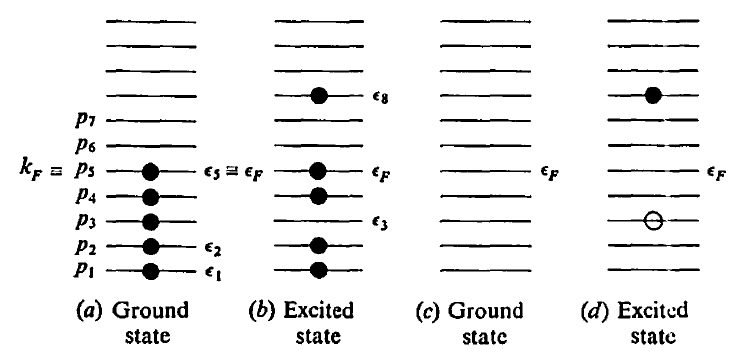
\includegraphics[scale=0.6]{screenshots/particle-hole.PNG}
    \caption{Non-interacting Fermi System}
    \label{fig:non-interacting-fermi}
\end{figure}
In the case where $U(\mathbf{r})=0$, the particles are free and $\mathbf{k}$ in \ref{fig:non-interacting-fermi}(a) are momentum, or wavenumber. The ground state of the single particle has energy $\epsilon_F$. If we now put N particles into the system, by Pauli principle the energy levels will be filled from the bottom as shown in \ref{fig:non-interacting-fermi}(a) for $N=5$. The highest filled energy level is the \textit{\textbf{Fermi level}},$\epsilon_F$. In ground state, the free particles fill a sphere in $\mathbf{k}-$space having radius $k_F=\sqrt{2m\epsilon_F}$,where $k_F$ is called the \textbf{Fermi momentum}. The filled sphere is called Fermi sea. The surface of this sphere is \textbf{Fermi surface}.

In Fig \ref{fig:non-interacting-fermi}(b) the excited states of the system are formed by removing a particle from a state below $\epsilon_F$ to a state above. The empty state here is called "hole". In "\bluep{particle-hole description}" we can omit the filled Fermi sea and only focus on excited particle and holes, yielding \ref{fig:non-interacting-fermi}(c) and (d). \textbf{\redp{Since a hole in state $\phi_k$ is actually removal of a particle from the system, the hole represents energy $\epsilon_k$ removed. Hence the hole energy is}}
\begin{equation}\epsilon_{k}^{\text {hole }}=-\epsilon_{k}\end{equation}
The time-dependent wave function is thus
\begin{equation}\psi_{k}(t)^{\text {hole }}=\phi_{k} e^{-i\left(-\epsilon_{k}\right) t}, \quad \epsilon_{k}<\epsilon_{F}\end{equation}
\subsection{A primer of second quantization formalism}
The total wave function for the ground and excited states of a system of non-interacting particles is the Slater determinant:
\begin{equation}\Phi_{k_{1}, \ldots, k_{N}}\left(\mathbf{r}_{1}, \ldots, \mathbf{r}_{N}\right)=\frac{1}{\sqrt{(N !)}}\left|\begin{array}{cc}
\phi_{k_{1}}\left(\mathbf{r}_{1}\right) \ldots \phi_{k_{1}}\left(\mathbf{r}_{N}\right) \\
\vdots & \vdots \\
\phi_{k_{N}}\left(\mathbf{r}_{1}\right) \ldots \phi_{k_{N}}\left(\mathbf{r}_{N}\right)
\end{array}\right|
\label{slater-determinant}
\end{equation}
\textbf{If the particles are allowed to interact with each other or external potential,} then the exact wave function of the system is a linear combination of \ref{slater-determinant}:
\begin{equation}\Psi\left(\mathbf{r}_{1}, \ldots, \mathbf{r}_{N}\right)=\sum_{k_{1}, \ldots, k_{N}} A_{k_{1}, \ldots, k_{N}} \Phi_{k_{1}, \ldots, k_{N}}\left(\mathbf{r}_{1}, \ldots, \mathbf{r}_{N}\right)\end{equation}
That is, the $\Phi_{k_1,k_2,\ldots}$ for the non-interacting system are the basis states used to describe the interacting system. Noting that all particles are indistinguishable, the essential information in \ref{slater-determinant} is just how many particles in each state, $n$. For short, we shall represent this as
\begin{equation}
    \Phi_{k_1,k_2,\ldots}=\left|n_{p_1},n_{p_2},\ldots\right\rangle
\label{linear-comb-occ-vec}
\end{equation}
meaning:$n_{p_{1}}$ particles in state $\phi_{p_{1}}, n_{p_{2}}$ in $\phi_{p_{3}},$ etc., where $n=0$ or 1 by Pauli principle. This notation is called "\redp{occupation number notation}". It is important to note that just as the original Slater determinant form a complete orthogonal set of basis functions, so do the states in occupation number notation and we have
\begin{equation}\left\langle n_{1}^{\prime}, \ldots n_{i}^{\prime} \ldots | n_{1}, \ldots, n_{i} \ldots\right\rangle=\delta_{n_1^{\prime}n_1}\ldots\delta_{n_i^{\prime}n_i}\ldots
\end{equation}
The wave function for interacting system is now becoming:
\begin{equation}\Psi=\sum_{n_{1}, \ldots, n_{i}, \ldots} A_{n_{1}, \ldots, n_{i}, \ldots}\left|n_{1}, \ldots, n_{i}, \ldots\right\rangle\end{equation}
In the particle-hole notation, it is necessary to introduce hole creation and destruction operators, $b_1^{\dagger}, b_{1}$, and similarly particle operators $a_1^{\dagger}, a_{1},$ as follows:
if $k_{i}<k_{F},$ then $c_{i}$ destroys a particle under the Fermi level, thus creating a hole. Hence
\begin{equation}\begin{aligned}
\text { for } k_{l}>k_{F}, & c_{l}=a_{l} \\
k_{l}<k_{F}, & c_{l}=b^{\dagger}_l
\end{aligned}\end{equation}
and
\begin{equation}\begin{aligned}
\text { for } k_{l}>k_{F}, & c_{l}^{\dagger}=a_{l}^{\dagger} \\
k_{l}<k_{F}, & c_{l}^{\dagger}=b_{l}
\end{aligned}\end{equation}
Simple examples of how the particle-hole operators work are:
$$a_{i}^{\dagger}|0\rangle=\left|1_i^{p}\right\rangle, \quad a_{i}\left|1_l^{p}\right\rangle=\delta_{il}|0\rangle, \quad b_{j}^{\dagger} a_{i}^{\dagger}\left|1_{m}^{\rho}\right\rangle=\left|1_{m}^{p}, 1_i^{p}, 1_j^{h}\right\rangle$$
where the superscripts represent "particle" and "hole", respectively. \redp{The operator in the occupation number formalism, $\mathcal{O}^{occ}$ is:}
\begin{equation}\mathcal{O}^{occ}=\sum_{m n} \mathcal{O}_{m n} c_{m}^{\dagger} c_{n}\end{equation}
where
\begin{equation}\begin{array}{l}
c_{l}=\theta_{k_{l}-k_{F}} a_{l}+\theta_{k_{F-k_{l}}} b_{l}^{\dagger} \\
c_{l}^{\dagger}=\theta_{k_{1}-k_{F}} a_{l}^{\dagger}+\theta_{k_{F}-k_{l}} b_{l}
\end{array}\end{equation}
and $\theta_{x}=1$ for $x>0 ; \quad \theta_{x}=0$ for $x<0$.

The Hamiltonian for an arbitrary system may be expressed in occupation number or particle-hole formalism. Suppose the system Hamiltonian in old Neanderthal notation describes a system in an external perturbing potential:
\begin{equation}H_{\text {Neand. }}=\underbrace{\sum_{i}\left[\frac{p_{1}^{2}}{2 m}+U\left(\mathbf{r}_{i}\right)\right]}_{H_{0}}+\underbrace{\sum_{i} V\left(\mathbf{r}_{i}\right)}_{H_{1}(\text { perturbation })}\end{equation}
The single-particle states $\phi_k$ satisfy:
\begin{equation}\left[\frac{p^{2}}{2 m}+U(\mathbf{r})\right] \phi_{k}=\epsilon_{k} \phi_{k}\end{equation}
Then it is found that
\begin{equation}H_{0}=\sum_{k} \epsilon_{k} c^{\dagger}_{k} c_{k}=\sum_{k>k_{F}} \epsilon_{k} a_{k}^{\dagger} a_{k}+\sum_{k<k_{F}} \epsilon_{k} b_{k} b^{\dagger}_{k}
\label{H0-Nead}
\end{equation}
\begin{equation}\begin{aligned}
H_{1}=& \sum_{m, n>k_{F}} V_{m n} a_{m}^{\dagger} a_{n}+\sum_{m>k_{F},n<k_F} V_{m n} a_{m}^{\dagger} b_{n}^{\dagger}+\sum_{m<k_{F}, n>k_{F}} V_{m n} b_{m} a_{n}+\\
&+\sum_{m, n<k_{F}} V_{m n} b_{m} b_{n}^{\dagger}
\end{aligned}
\label{H1}
\end{equation}
For a system of mutually interacting particles with a Hamiltonian
\begin{equation}H_{\mathrm{old}}=\underbrace{\sum_{l} \frac{p_{l}^{2}}{2 m}}_{H_{0}}+\frac{1}{2} \underbrace{\sum_{i, J} V\left(\mathbf{r}_{i}-\mathbf{r}_{j}\right)}_{H_{1}(\text { perturbation })}
\label{mutual-interact-hamiltonian}
\end{equation}
We also find that
\begin{equation}H_{0}=\sum_{k>k_{F}} \epsilon_{k} a_{k}^{\dagger} a_{k}+\sum_{k<k_{F}} \epsilon_{k} b_{k} b^{\dagger}_{k}\quad\epsilon_k=k^2/2m\end{equation}
\begin{equation}\begin{aligned}
H_{1}&=\frac{1}{2} \sum_{k, l, m, n>k_{F}} V_{k l m n} a_{l}^{\dagger} a_{k}^{\dagger} a_{m} a_{n}+\sum_{k, l, m>k_{F};n<k_F} V_{k l m n} a_{l}^{\dagger} a^{\dagger}_{k} a_{m} b_{n}^{\dagger}+\\
&+\cdots+\frac{1}{2} \sum_{k, l, m, n<k_{r}} V_{k l m n} b_{l} b_{k} b_{m}^{\dagger} b_{n}^{\dagger}
\end{aligned}
\label{mutual-interact-H1}
\end{equation}
We will define $V_{klmn}$ later. It should be carefully remembered that \textbf{\bluep{in the case of interacting system, the wave functions  are given by the linear combination of \ref{linear-comb-occ-vec}.}}

\subsection{Propagator for non-interacting Fermi system in external perturbing potential}
To treat the general situation of "holes", we extend the definition of propagator to times $t_2<t_1$. This leads us to the definition:
\begin{imp}
\begin{equation}
    iG(k_2,k_1,t_2-t_1)_{t_2<t_1}\equiv i G^{-}\left(k_{2}, k_{1}, t_{2}-t_{1}\right)
\end{equation}
which is $-1\times$probability amplitude that if at time $t_{2}$ we remove a particle in state $\phi_{k_{2}}$ from (i.e., if we add a hole in $\phi_{k_{2}}$ to) the interacting system in its ground state, then at time $t_{1}$ the system will be in its ground state with a particle removed from (i.e., an added hole in $) \phi_{k_{1}}$.\bluep{ The factor of (-1) here compared with $iG^+$ comes because we have fermions. Note that $G^-$ is called an "advanced" propagator or Green's function.}
\end{imp}
\redp{for $\left.t_{2}>t_{1} \text { (but not for } t_{2}=t_{1} !\right), G^{-}$ is defined so that}
\begin{equation}i G^{-}\left(k_{2}, k_{1}, t_{2}-t_{1}\right)_{t_{2}>r_{1}}=0\end{equation}

In the case of a free hole, we have
\begin{equation}G_{0}^{-}\left(k, t_{2}-t_{1}\right)=\left\{\begin{array}{l}
i \theta_{t_{1}-t_{2}} e^{-i \epsilon_{k}\left(t_{2}-t_{1}\right)}\quad t_2\neq t1,\epsilon_k<\epsilon_F \\
i, \quad \text { for } t_{2}=t_{1}
\end{array}\right.
\label{Gminus-t-space}
\end{equation}
with Fourier transform
\begin{equation}G_{0}^{-}(k, \omega)=\frac{1}{\omega-\epsilon_{k}-i \delta}, \quad \epsilon_{k}<\epsilon_{F}
\label{Gminus-k-space}
\end{equation}
The interaction amplitude, $V_{kl}$, merits some discussion. It is given by 
\begin{equation}V_{k l}=\int d^{3} \mathbf{r} \phi_{k}^{*}(\mathbf{r}) V(\mathbf{r}, \mathbf{p}) \phi_{l}(\mathbf{r})
\label{Vkl}
\end{equation}
There are four possibilities of $V_{kl}$ shown in the table below. They mean:(a) scattering of a particle in particle-hole formalism from state $\phi_{l}$ to $\phi_{k},$ (b) the potential scatters a particle out of state $\phi_{l},$ where $\epsilon_{l}<\epsilon_{F},$ into state $\phi_{k}, \epsilon_{k}>\epsilon_{F},$ thus simultaneously creating a particle in $\phi_{k}$ and a hole in $\phi_{l},(c),$ etc. \redp{Note that these four possibilities correspond to the four interaction terms in the particle-hole Hamiltonian for this case (\ref{mutual-interact-hamiltonian})}.
\begin{figure}[H]
    \centering
\tikzset{every picture/.style={line width=0.75pt}} %set default line width to 0.75pt        
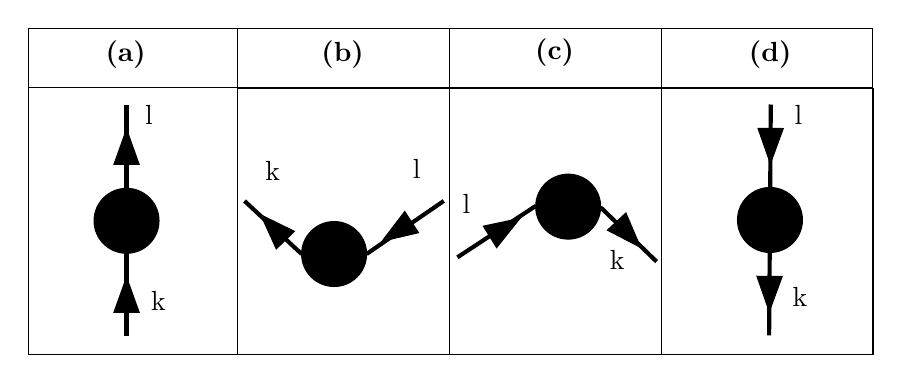
\begin{tikzpicture}[x=0.75pt,y=0.75pt,yscale=-1,xscale=1]
%uncomment if require: \path (0,244); %set diagram left start at 0, and has height of 244

%Shape: Circle [id:dp7355643708429443] 
\draw  [fill={rgb, 255:red, 0; green, 0; blue, 0 }  ,fill opacity=1 ] (147.73,133.97) .. controls (147.73,125.33) and (154.73,118.33) .. (163.37,118.33) .. controls (172,118.33) and (179,125.33) .. (179,133.97) .. controls (179,142.6) and (172,149.6) .. (163.37,149.6) .. controls (154.73,149.6) and (147.73,142.6) .. (147.73,133.97) -- cycle ;
%Straight Lines [id:da3859042750603179] 
\draw [line width=1.5]    (163.37,149.6) -- (163.37,189.6) ;
%Straight Lines [id:da7654556741518936] 
\draw [line width=1.5]    (163.37,78.33) -- (163.37,118.33) ;
%Shape: Triangle [id:dp19291169740752956] 
\draw  [fill={rgb, 255:red, 0; green, 0; blue, 0 }  ,fill opacity=1 ] (163.37,89.87) -- (169.43,106.79) -- (157.3,106.79) -- cycle ;
%Shape: Triangle [id:dp3466064725515261] 
\draw  [fill={rgb, 255:red, 0; green, 0; blue, 0 }  ,fill opacity=1 ] (163.37,161.14) -- (169.43,178.06) -- (157.3,178.06) -- cycle ;
%Shape: Circle [id:dp605096323889595] 
\draw  [fill={rgb, 255:red, 0; green, 0; blue, 0 }  ,fill opacity=1 ] (247.73,149.97) .. controls (247.73,141.33) and (254.73,134.33) .. (263.37,134.33) .. controls (272,134.33) and (279,141.33) .. (279,149.97) .. controls (279,158.6) and (272,165.6) .. (263.37,165.6) .. controls (254.73,165.6) and (247.73,158.6) .. (247.73,149.97) -- cycle ;
%Straight Lines [id:da59504555135735] 
\draw [line width=1.5]    (279,149.97) -- (316.2,124.4) ;
%Straight Lines [id:da3713869779792379] 
\draw [line width=1.5]    (220.2,124.4) -- (247.73,149.97) ;
%Shape: Triangle [id:dp6549052988211023] 
\draw  [fill={rgb, 255:red, 0; green, 0; blue, 0 }  ,fill opacity=1 ] (228.08,131.11) -- (244.21,139.04) -- (235.5,147.48) -- cycle ;
%Shape: Triangle [id:dp6944058778949381] 
\draw  [fill={rgb, 255:red, 0; green, 0; blue, 0 }  ,fill opacity=1 ] (286.5,143.78) -- (297.41,129.5) -- (304,139.68) -- cycle ;
%Shape: Circle [id:dp5744676253853855] 
\draw  [fill={rgb, 255:red, 0; green, 0; blue, 0 }  ,fill opacity=1 ] (391.77,127.47) .. controls (391.58,136.11) and (384.44,142.95) .. (375.8,142.77) .. controls (367.17,142.58) and (360.32,135.43) .. (360.51,126.8) .. controls (360.69,118.17) and (367.84,111.32) .. (376.47,111.51) .. controls (385.11,111.69) and (391.95,118.84) .. (391.77,127.47) -- cycle ;
%Straight Lines [id:da9080029217596884] 
\draw [line width=1.5]    (360.51,126.8) -- (322.77,151.56) ;
%Straight Lines [id:da5417814826950174] 
\draw [line width=1.5]    (418.75,153.63) -- (391.77,127.47) ;
%Shape: Triangle [id:dp21341953231164135] 
\draw  [fill={rgb, 255:red, 0; green, 0; blue, 0 }  ,fill opacity=1 ] (411.01,146.75) -- (395.06,138.48) -- (403.95,130.22) -- cycle ;
%Shape: Triangle [id:dp18680249773366642] 
\draw  [fill={rgb, 255:red, 0; green, 0; blue, 0 }  ,fill opacity=1 ] (352.88,132.83) -- (341.67,146.87) -- (335.3,136.55) -- cycle ;
%Shape: Circle [id:dp23848631002762677] 
\draw  [fill={rgb, 255:red, 0; green, 0; blue, 0 }  ,fill opacity=1 ] (489,133.68) .. controls (488.94,142.32) and (481.89,149.26) .. (473.25,149.2) .. controls (464.62,149.14) and (457.67,142.09) .. (457.73,133.45) .. controls (457.8,124.82) and (464.85,117.87) .. (473.48,117.93) .. controls (482.12,118) and (489.06,125.05) .. (489,133.68) -- cycle ;
%Straight Lines [id:da48621128625100807] 
\draw [line width=1.5]    (473.48,117.93) -- (473.77,77.93) ;
%Straight Lines [id:da07279871641659819] 
\draw [line width=1.5]    (472.96,189.2) -- (473.25,149.2) ;
%Shape: Triangle [id:dp6526600818062779] 
\draw  [fill={rgb, 255:red, 0; green, 0; blue, 0 }  ,fill opacity=1 ] (473.04,177.66) -- (467.1,160.7) -- (479.23,160.79) -- cycle ;
%Shape: Triangle [id:dp49414286713798516] 
\draw  [fill={rgb, 255:red, 0; green, 0; blue, 0 }  ,fill opacity=1 ] (473.57,106.39) -- (467.62,89.43) -- (479.76,89.52) -- cycle ;
%Shape: Rectangle [id:dp23062556048857352] 
\draw   (116,69.87) -- (217,69.87) -- (217,198.18) -- (116,198.18) -- cycle ;
%Shape: Rectangle [id:dp4116028056497356] 
\draw   (217,70.18) -- (319,70.18) -- (319,198.18) -- (217,198.18) -- cycle ;
%Shape: Rectangle [id:dp7757074524824593] 
\draw   (319,70.18) -- (421,70.18) -- (421,198.18) -- (319,198.18) -- cycle ;
%Shape: Rectangle [id:dp537554675418955] 
\draw   (421,70.18) -- (523,70.18) -- (523,198.18) -- (421,198.18) -- cycle ;
%Shape: Rectangle [id:dp8001518431361148] 
\draw   (116,41.18) -- (217,41.18) -- (217,69.87) -- (116,69.87) -- cycle ;
%Shape: Rectangle [id:dp6414334269575042] 
\draw   (217,41.18) -- (318.95,41.18) -- (318.95,69.87) -- (217,69.87) -- cycle ;
%Shape: Rectangle [id:dp059392457734880444] 
\draw   (318.95,41.18) -- (420.9,41.18) -- (420.9,69.87) -- (318.95,69.87) -- cycle ;
%Shape: Rectangle [id:dp2648624460179885] 
\draw   (420.9,41.18) -- (522.85,41.18) -- (522.85,69.87) -- (420.9,69.87) -- cycle ;

% Text Node
\draw (152,45.85) node [anchor=north west][inner sep=0.75pt]   [align=left] {\textbf{(a)}};
% Text Node
\draw (256,45.85) node [anchor=north west][inner sep=0.75pt]   [align=left] {\textbf{(b)}};
% Text Node
\draw (359,44.85) node [anchor=north west][inner sep=0.75pt]   [align=left] {\textbf{(c)}};
% Text Node
\draw (462,45.85) node [anchor=north west][inner sep=0.75pt]   [align=left] {\textbf{(d)}};
% Text Node
\draw (174,166.85) node [anchor=north west][inner sep=0.75pt]   [align=left] {k};
% Text Node
\draw (171,76.85) node [anchor=north west][inner sep=0.75pt]   [align=left] {l};
% Text Node
\draw (300,102.85) node [anchor=north west][inner sep=0.75pt]   [align=left] {l};
% Text Node
\draw (324,119.85) node [anchor=north west][inner sep=0.75pt]   [align=left] {l};
% Text Node
\draw (484,76.85) node [anchor=north west][inner sep=0.75pt]   [align=left] {l};
% Text Node
\draw (229,103.85) node [anchor=north west][inner sep=0.75pt]   [align=left] {k};
% Text Node
\draw (395,146.85) node [anchor=north west][inner sep=0.75pt]   [align=left] {k};
% Text Node
\draw (483,164.85) node [anchor=north west][inner sep=0.75pt]   [align=left] {k};


\end{tikzpicture}
    \caption{Kinds of $iV_{kl}$}
    \label{fig:Vkl-table}
\end{figure}
With the aid of the table above, the diagrammatic series for $G^+$ may be drawn as the sum of all possible diagrams which can be built up out of sequences of interaction dots connected by particle and hole lines:
\begin{equation}
    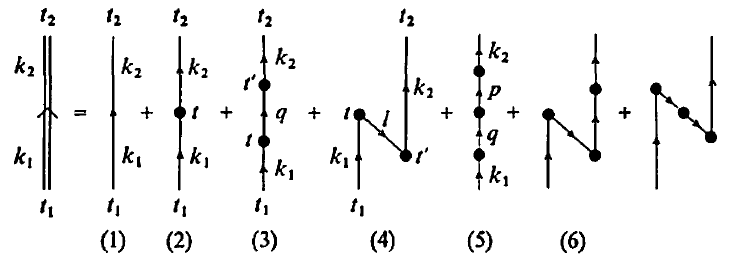
\includegraphics[width=0.8\textwidth]{screenshots/Goldstone-digram-series.PNG}\mathbf{+\ldots}
    \label{dots-line-series}
\end{equation}
The first diagram disappear if $k_2\neq k_1$. Look at the fourth diagram. A particle enters the system in state $k_{1}\left(\equiv \phi_{k_{1}}\right)$ at time $t_{1}$. At time $t^{\prime},$ the potential knocks a particle out of the state $l$ into state $k_{2}$ thus creating a particle in $k_{2}$ and a hole in $l$. At time $t,$ the particle in $k_{1}$ is knocked into the hole in $l$ causing mutual annihilation; the particle in $k_{2}$ continues propagating until $t_{2}$.

It should be pointed out that many diagrams in this series \textbf{violate the Pauli exclusion principle}. For example, when $k_{1}=k_{2},$ in diagram 4 we have two particles in the same state, $k_{1}$. The reason why such diagrams must be included is explained later. It's included here mainly to make the math correct. Translate the diagram (4) into equations, we have:

(1) Put in particle in state $k_1$ at time $t_1$:
$$a_{k_{1}}|0\rangle=\left|1_{k_{1}}\right\rangle$$

(2) At $t^{\prime},$ one of the terms in $H_{1}$ acts on system creating particle in $k_{2},$ hole in $l:$
$$V_{k_{2}l}, a^{\dagger}_{k_{2}} b_{l}^{\dagger}\left|1^p_{k_1}\right\rangle=V_{k_{2}l} \left| 1^p_{k_{1}}, 1^h_l, 1^p_{k_2}\right\rangle$$

(3) At $t, H_{1}$ acts again, destroying hole in $l,$ particle in $k_{1}$:
$$
V_{lk_1}b_la_{k_1}[V_{k_2l}| 1^p_{k_{1}}, 1^h_l, 1^p_{k_2}\rangle]=V_{k_2l}V_{lk_1}|1^p_{k_2}\rangle
$$

(4) At $t_2$, take the particle out:
$$
a_{k_2}[V_{k_2l}V_{lk_1}|1^P_{k_2}\rangle]=V_{k_2l}V_{lk_1}|0\rangle
$$
The above diagram series may be written out in words in (k,t) space:
\begin{equation}\begin{aligned}
G^{+}\left(k_{2}, k_{1}, t_{2}-t_{1}\right)=G_{0}^{+}\left(k_{1}, t_{2}-t_{1}\right) \delta_{k_{1}k_{2}}  \\
&+\int_{-\infty}^{+\infty} d t G_{0}^{+}\left(k_{2}, t_{2}-t\right) V_{k_{2} k_{1}} G_{0}^{+}\left(k_{1}, t-t_{1}\right)+\\
&+\sum_{q>k_{F}} \int_{-\infty}^{\infty} d t \int_{-\infty}^{\infty} d t^{\prime} \cdots+\cdots
\end{aligned}
\label{time-int-goldstone}
\end{equation}
In ($k,\omega$) space:
\begin{equation}\begin{array}{rl}
G^{+}\left(k_{2}, k_{1}\right)=\delta_{k_{1}k_{2}} &  G_{0}^{+}\left(k_{1}\right)+G_{0}^{+}\left(k_{1}\right) V_{k_{2} k_{1}} G_{0}^{+}\left(k_{2}\right) \\
& +\sum_{q>k_{F}} G_{0}^{+}\left(k_{1}\right) V_{q k_{1}} G_{0}^{+}(q) V_{k_{2} q} G_{0}^{+}\left(k_{2}\right)+ \\
& +\sum_{l<k_{F}} G_{0}^{+}\left(k_{1}\right) V_{l k_{1}} G_{0}^{-}(l) V_{k_{2}l}, G_{0}^{+}\left(k_{2}\right)+\cdots
\end{array}
\label{omega-int-goldstone}
\end{equation}
And now an easy example showing how to evaluate $G^+$ by partial summation. Suppose $k_1=k_2=k(k>k_F)$, and the potential is such that $V_{mk}$ and $V_{km}$($\epsilon_m<\epsilon_F$) are large, and all the other $V$'s are small. Then the propagator in \ref{omega-int-goldstone} may be approximated by the sum of the following diagrams:
\begin{equation}
\begin{aligned}
&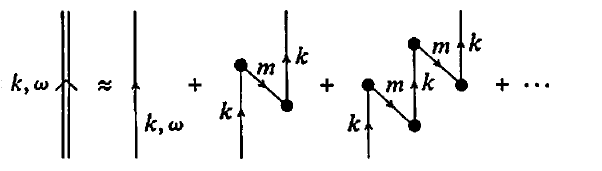
\includegraphics[width=0.8\textwidth]{screenshots/partial-Vmk-series.PNG}\\
&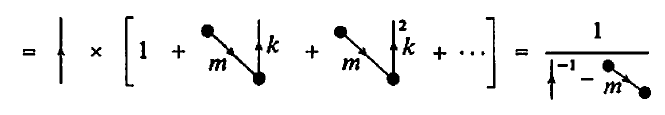
\includegraphics[width=0.8\textwidth]{screenshots/partial-Vmk-series2.PNG}
\end{aligned}
\end{equation}
Thus
\begin{equation}\begin{aligned}
G^{+}(k, \omega) &=\frac{1}{\left[G_{0}^{+}(k, \omega)\right]^{-1}-V_{k m} V_{m k} G_{0}^{-}(m, \omega)} \\
&=\frac{1}{\left(\omega-\epsilon_{k}+i \delta\right)-\frac{\left|V_{k m}\right|^{2}}{\left(\omega-\epsilon_{m}-i \delta\right)}}
\end{aligned}\end{equation}
\redp{\textbf{Dropping the $i\delta$'s(they have no significance in this simple calculation) yields}}
$$\omega-\epsilon_{k}-\frac{\left|V_{k m}\right|^{2}}{\omega-\epsilon_{m}}=0$$
$$\begin{aligned}
\omega &=\epsilon_{k}^{\prime}=\frac{\epsilon_{k}+\epsilon_{m}}{2}+\frac{1}{2} \sqrt{\left\{\left(\epsilon_{k}-\epsilon_{m}\right)^{2}+4\left|V_{k m}\right|^{2}\right\}} \\
&=\epsilon_{m}^{\prime}=\frac{\epsilon_{k}+\epsilon_{m}}{2}-\frac{1}{2} \sqrt{\{(\epsilon_{k}-\epsilon_{m})^{2}+4|V_{k m}|^{2}\}}
\end{aligned}$$
Note that \bluep{the summation must go to infinite order to get quasi-particle energies. Any finite order will still lead to the unperturbed energies.}

\subsection{Interacting Fermi system}
Imagine now we have a system consisting of N fermions interacting by means of two-body forces $V(|\mathbf{r}_i-\mathbf{r}_j|)$. Assume there is no external fields, so that the single particle states are just $\phi_{k}=\Omega^{-1/2} \exp (i \mathbf{k} \cdot \mathbf{r})$ with $\epsilon_k=k^2/2m$. The object of this section is to construct diagramatically the perturbation expansion of the propagator for this system, evaluate it by partial summation and examine the result for quasi particle behavior.

The first thing is to find the transition probability amplitude for a process in which two particles, one in state $\phi_{m},$ the other in state $\phi_{n}$ collide with each other and are scattered into states $\phi_{k}, \phi_{l}$ respectively. Analogous to the interaction amplitude $V_{k l}$, this is just the matrix element
\begin{equation}
V_{k l m n}=\int d^{3} \mathbf{r} \int d^{3} \mathbf{r}^{\prime} \phi_{k}^{*}(\mathbf{r}) \phi_{l}^{*}\left(\mathbf{r}^{\prime}\right) V\left(\left|\mathbf{r}-\mathbf{r}^{\prime}\right|\right) \phi_{m}(\mathbf{r}) \phi_{n}\left(\mathbf{r}^{\prime}\right)=V_{i k n m}
\label{Vklmn-defi}
\end{equation}
Such interaction may be represented diagrammatically by a wiggly line:
\begin{center}
\tikzset{every picture/.style={line width=0.75pt}} %set default line width to 0.75pt        
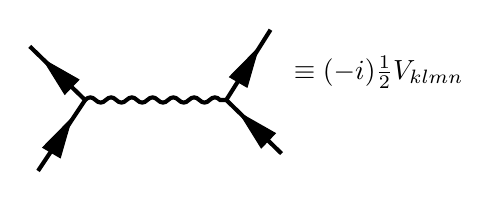
\begin{tikzpicture}[x=0.75pt,y=0.75pt,yscale=-1,xscale=1]
%uncomment if require: \path (0,705); %set diagram left start at 0, and has height of 705
%Straight Lines [id:da613823184290475] 
\draw [line width=1.5]    (436.42,562.13) .. controls (438.09,560.46) and (439.75,560.46) .. (441.42,562.13) .. controls (443.09,563.8) and (444.75,563.8) .. (446.42,562.13) .. controls (448.09,560.46) and (449.75,560.46) .. (451.42,562.13) .. controls (453.09,563.8) and (454.75,563.8) .. (456.42,562.13) .. controls (458.09,560.46) and (459.75,560.46) .. (461.42,562.13) .. controls (463.09,563.8) and (464.75,563.8) .. (466.42,562.13) .. controls (468.09,560.46) and (469.75,560.46) .. (471.42,562.13) .. controls (473.09,563.8) and (474.75,563.8) .. (476.42,562.13) .. controls (478.09,560.46) and (479.75,560.46) .. (481.42,562.13) .. controls (483.09,563.8) and (484.75,563.8) .. (486.42,562.13) .. controls (488.09,560.46) and (489.75,560.46) .. (491.42,562.13) .. controls (493.09,563.8) and (494.75,563.8) .. (496.42,562.13) .. controls (498.09,560.46) and (499.75,560.46) .. (501.42,562.13) -- (504.42,562.13) -- (504.42,562.13) ;
%Straight Lines [id:da6353755682299548] 
\draw [line width=1.5]    (409.75,536.3) -- (436.42,562.13) ;
%Straight Lines [id:da6254606220772768] 
\draw [line width=1.5]    (504.42,562.13) -- (531.08,587.97) ;
%Straight Lines [id:da5480869883300985] 
\draw [line width=1.5]    (436.42,562.13) -- (413.75,596.3) ;
%Straight Lines [id:da49445752084181116] 
\draw [line width=1.5]    (525.75,528.3) -- (504.42,562.13) ;
%Shape: Triangle [id:dp022384072825595847] 
\draw  [fill={rgb, 255:red, 0; green, 0; blue, 0 }  ,fill opacity=1 ] (416.18,542.57) -- (433.37,552.35) -- (426.61,559.37) -- cycle ;
%Shape: Triangle [id:dp5669679661948073] 
\draw  [fill={rgb, 255:red, 0; green, 0; blue, 0 }  ,fill opacity=1 ] (510.84,568.41) -- (528.04,578.18) -- (521.28,585.21) -- cycle ;
%Shape: Triangle [id:dp23872151900315752] 
\draw  [fill={rgb, 255:red, 0; green, 0; blue, 0 }  ,fill opacity=1 ] (519.92,536.94) -- (514.46,555.95) -- (506.04,551.03) -- cycle ;
%Shape: Triangle [id:dp5504301680867448] 
\draw  [fill={rgb, 255:red, 0; green, 0; blue, 0 }  ,fill opacity=1 ] (429.92,570.94) -- (424.46,589.95) -- (416.04,585.03) -- cycle ;

% Text Node
\draw (535.68,539.7) node [anchor=north west][inner sep=0.75pt]    {$\equiv ( -i)\frac{1}{2} V_{klmn}$};
\end{tikzpicture}
\end{center}
Using the particle-hole formalism, this may be drawn in more detail, thus:
\begin{equation}
    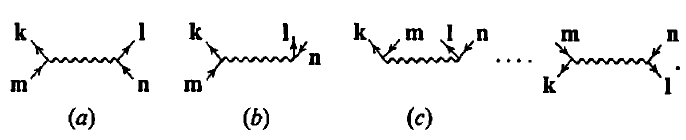
\includegraphics[width=0.8\textwidth]{screenshots/wiggly-diagram-types.PNG}
    \label{wiggly-types}
\end{equation}
Diagram (a) pictures scattering of two particles at state $\phi_m$ and $\phi_n$ into $\phi_k$ and $\phi_l$. In (b) a particle at state $\phi_m$ interacts with another particle below the Fermi surface in state $\phi_n$ to create a hole in $\phi_n$ and a particle in $\phi_l$. At the same time the original particle undergoes a transition to state $\phi_k$. Note that the diagrams in \ref{wiggly-types} correspond precisely to the interaction terms in the Hamiltonian of \ref{mutual-interact-hamiltonian}.
\begin{imp}
It is extremely important to note the labelling convention used in $V_{k l m n}: \mathbf{k}=$ line out of left vertex, $\mathbf{l}=$ line out of right vertex, $\mathbf{m}=$ line into left vertex, $\mathbf{n}=$ line into right vertex. A mnemonic aid is to remember the tango dance step: \textbf{left out, right out, left in, right in.}
\end{imp}
\redp{The interaction $V(|\mathbf{r}-\mathbf{r}^{\prime}|)$ only depends on the distance between the particles so it conserves linear and spin momentum.} Thus
$$\mathbf{k}+\mathbf{l}=\mathbf{m}+\mathbf{n} ; \quad \boldsymbol{\sigma}_{k}+\boldsymbol{\sigma}_{l}=\boldsymbol{\sigma}_{m}+\boldsymbol{\sigma}_{n}$$
We can incorporate this conservation law into our diagrams by labelling the "momentum flow" shown below:
\begin{equation}
\tikzset{every picture/.style={line width=0.75pt}} %set default line width to 0.75pt        
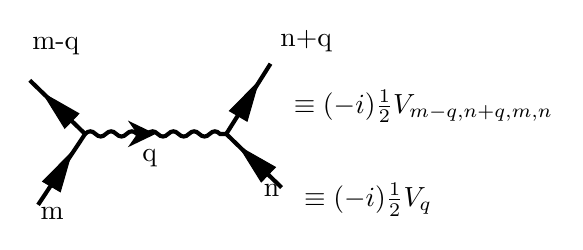
\begin{tikzpicture}[x=0.75pt,y=0.75pt,yscale=-1,xscale=1]
%uncomment if require: \path (0,705); %set diagram left start at 0, and has height of 705
%Straight Lines [id:da613823184290475] 
\draw [line width=1.5]    (416.42,563.13) .. controls (418.09,561.46) and (419.75,561.46) .. (421.42,563.13) .. controls (423.09,564.8) and (424.75,564.8) .. (426.42,563.13) .. controls (428.09,561.46) and (429.75,561.46) .. (431.42,563.13) .. controls (433.09,564.8) and (434.75,564.8) .. (436.42,563.13) .. controls (438.09,561.46) and (439.75,561.46) .. (441.42,563.13) .. controls (443.09,564.8) and (444.75,564.8) .. (446.42,563.13) .. controls (448.09,561.46) and (449.75,561.46) .. (451.42,563.13) .. controls (453.09,564.8) and (454.75,564.8) .. (456.42,563.13) .. controls (458.09,561.46) and (459.75,561.46) .. (461.42,563.13) .. controls (463.09,564.8) and (464.75,564.8) .. (466.42,563.13) .. controls (468.09,561.46) and (469.75,561.46) .. (471.42,563.13) .. controls (473.09,564.8) and (474.75,564.8) .. (476.42,563.13) .. controls (478.09,561.46) and (479.75,561.46) .. (481.42,563.13) -- (484.42,563.13) -- (484.42,563.13) ;
\draw [shift={(450.42,563.13)}, rotate = 180] [fill={rgb, 255:red, 0; green, 0; blue, 0 }  ][line width=0.08]  [draw opacity=0] (13.4,-6.43) -- (0,0) -- (13.4,6.44) -- (8.9,0) -- cycle    ;
%Straight Lines [id:da6353755682299548] 
\draw [line width=1.5]    (389.75,537.3) -- (416.42,563.13) ;
%Straight Lines [id:da6254606220772768] 
\draw [line width=1.5]    (484.42,563.13) -- (511.08,588.97) ;
%Straight Lines [id:da5480869883300985] 
\draw [line width=1.5]    (416.42,563.13) -- (393.75,597.3) ;
%Straight Lines [id:da49445752084181116] 
\draw [line width=1.5]    (505.75,529.3) -- (484.42,563.13) ;
%Shape: Triangle [id:dp022384072825595847] 
\draw  [fill={rgb, 255:red, 0; green, 0; blue, 0 }  ,fill opacity=1 ] (396.18,543.57) -- (413.37,553.35) -- (406.61,560.37) -- cycle ;
%Shape: Triangle [id:dp5669679661948073] 
\draw  [fill={rgb, 255:red, 0; green, 0; blue, 0 }  ,fill opacity=1 ] (490.84,569.41) -- (508.04,579.18) -- (501.28,586.21) -- cycle ;
%Shape: Triangle [id:dp23872151900315752] 
\draw  [fill={rgb, 255:red, 0; green, 0; blue, 0 }  ,fill opacity=1 ] (499.92,537.94) -- (494.46,556.95) -- (486.04,552.03) -- cycle ;
%Shape: Triangle [id:dp5504301680867448] 
\draw  [fill={rgb, 255:red, 0; green, 0; blue, 0 }  ,fill opacity=1 ] (409.92,571.94) -- (404.46,590.95) -- (396.04,586.03) -- cycle ;

% Text Node
\draw (515.68,540.7) node [anchor=north west][inner sep=0.75pt]    {$\equiv ( -i)\frac{1}{2} V_{m-q,n+q,m,n}$};
% Text Node
\draw (393.75,597.3) node [anchor=north west][inner sep=0.75pt]   [align=left] {m};
% Text Node
\draw (389.75,515.3) node [anchor=north west][inner sep=0.75pt]   [align=left] {m-q};
% Text Node
\draw (442.75,569.3) node [anchor=north west][inner sep=0.75pt]   [align=left] {q};
% Text Node
\draw (501.28,586.21) node [anchor=north west][inner sep=0.75pt]   [align=left] {n};
% Text Node
\draw (509.28,512.21) node [anchor=north west][inner sep=0.75pt]   [align=left] {n+q};
% Text Node
\draw (520.68,585.7) node [anchor=north west][inner sep=0.75pt]    {$\equiv ( -i)\frac{1}{2} V_{q}$};


\end{tikzpicture}
\label{momentum-flow}
\end{equation}
By changing the dummy indices in \ref{Vklmn-defi} we have $V_{klmn}=V_{lknm}$, so $V_q=V_{-q}$. $V_{-q}$ corresponds to the diagram in \ref{momentum-flow} twisted through $180^o$, has momentum transfer $\mathbf{q}^{\prime}=\mathbf{n}-\mathbf{l}$.
\begin{imp}
It is important to note that although the collisions conserves momentum, they do not conserve energy. For example, at the lower interaction of the diagram shown below we see the energy flow into the interaction \bluep{(in the unit of $\hbar^2/2m$)} is $k^2+l^2$, while the energy flow out is $(k-q)^2+(l+q)^2$. Hence we are dealing with virtual particles during the interactions.
\begin{center}
    


\tikzset{every picture/.style={line width=0.75pt}} %set default line width to 0.75pt        

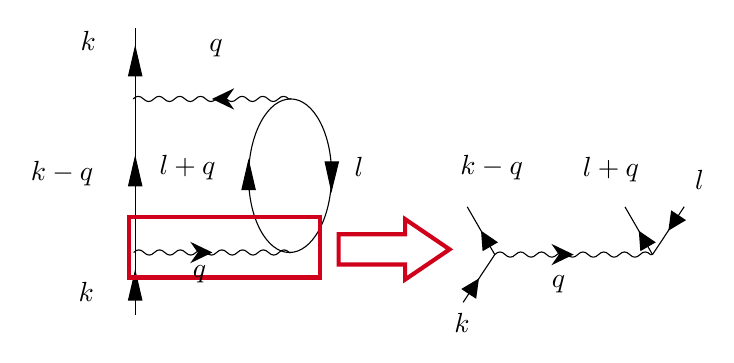
\begin{tikzpicture}[x=0.75pt,y=0.75pt,yscale=-1,xscale=1]
%uncomment if require: \path (0,244); %set diagram left start at 0, and has height of 244

%Straight Lines [id:da8265491360075683] 
\draw    (62.53,30.8) -- (62.53,168.8) ;
%Straight Lines [id:da7214893814207295] 
\draw    (61.53,64.8) .. controls (63.2,63.13) and (64.86,63.13) .. (66.53,64.8) .. controls (68.2,66.47) and (69.86,66.47) .. (71.53,64.8) .. controls (73.2,63.13) and (74.86,63.13) .. (76.53,64.8) .. controls (78.2,66.47) and (79.86,66.47) .. (81.53,64.8) .. controls (83.2,63.13) and (84.86,63.13) .. (86.53,64.8) .. controls (88.2,66.47) and (89.86,66.47) .. (91.53,64.8) .. controls (93.2,63.13) and (94.86,63.13) .. (96.53,64.8) .. controls (98.2,66.47) and (99.86,66.47) .. (101.53,64.8) .. controls (103.2,63.13) and (104.86,63.13) .. (106.53,64.8) .. controls (108.2,66.47) and (109.86,66.47) .. (111.53,64.8) .. controls (113.2,63.13) and (114.86,63.13) .. (116.53,64.8) .. controls (118.2,66.47) and (119.86,66.47) .. (121.53,64.8) .. controls (123.2,63.13) and (124.86,63.13) .. (126.53,64.8) .. controls (128.2,66.47) and (129.86,66.47) .. (131.53,64.8) .. controls (133.2,63.13) and (134.86,63.13) .. (136.53,64.8) -- (137.53,64.8) -- (137.53,64.8) ;
\draw [shift={(99.53,64.8)}, rotate = 0] [fill={rgb, 255:red, 0; green, 0; blue, 0 }  ][line width=0.08]  [draw opacity=0] (10.72,-5.15) -- (0,0) -- (10.72,5.15) -- (7.12,0) -- cycle    ;
%Straight Lines [id:da6531867980247327] 
\draw    (61.78,138.78) .. controls (63.45,137.11) and (65.11,137.11) .. (66.78,138.78) .. controls (68.45,140.45) and (70.11,140.45) .. (71.78,138.78) .. controls (73.45,137.11) and (75.11,137.11) .. (76.78,138.78) .. controls (78.45,140.45) and (80.11,140.45) .. (81.78,138.78) .. controls (83.45,137.11) and (85.11,137.11) .. (86.78,138.78) .. controls (88.45,140.45) and (90.11,140.45) .. (91.78,138.78) .. controls (93.45,137.11) and (95.11,137.11) .. (96.78,138.78) .. controls (98.45,140.45) and (100.11,140.45) .. (101.78,138.78) .. controls (103.45,137.11) and (105.11,137.11) .. (106.78,138.78) .. controls (108.45,140.45) and (110.11,140.45) .. (111.78,138.78) .. controls (113.45,137.11) and (115.11,137.11) .. (116.78,138.78) .. controls (118.45,140.45) and (120.11,140.45) .. (121.78,138.78) .. controls (123.45,137.11) and (125.11,137.11) .. (126.78,138.78) .. controls (128.45,140.45) and (130.11,140.45) .. (131.78,138.78) .. controls (133.45,137.11) and (135.11,137.11) .. (136.78,138.78) -- (137.78,138.78) -- (137.78,138.78) ;
\draw [shift={(99.78,138.78)}, rotate = 180] [fill={rgb, 255:red, 0; green, 0; blue, 0 }  ][line width=0.08]  [draw opacity=0] (10.72,-5.15) -- (0,0) -- (10.72,5.15) -- (7.12,0) -- cycle    ;
%Shape: Ellipse [id:dp27679763462197615] 
\draw   (136.78,138.78) .. controls (125.74,138.67) and (116.95,122.02) .. (117.16,101.59) .. controls (117.37,81.16) and (126.49,64.69) .. (137.53,64.8) .. controls (148.58,64.91) and (157.36,81.56) .. (157.16,101.99) .. controls (156.95,122.42) and (147.83,138.89) .. (136.78,138.78) -- cycle ;
%Shape: Triangle [id:dp5635326143074989] 
\draw  [fill={rgb, 255:red, 0; green, 0; blue, 0 }  ,fill opacity=1 ] (117.16,94.73) -- (120.35,108.45) -- (113.97,108.45) -- cycle ;
%Shape: Triangle [id:dp24603935178928227] 
\draw  [fill={rgb, 255:red, 0; green, 0; blue, 0 }  ,fill opacity=1 ] (157.07,108.86) -- (154.06,95.09) -- (160.44,95.17) -- cycle ;
%Shape: Triangle [id:dp6426129992054267] 
\draw  [fill={rgb, 255:red, 0; green, 0; blue, 0 }  ,fill opacity=1 ] (62.53,92.94) -- (65.72,106.66) -- (59.35,106.66) -- cycle ;
%Shape: Triangle [id:dp6567192777691618] 
\draw  [fill={rgb, 255:red, 0; green, 0; blue, 0 }  ,fill opacity=1 ] (62.53,39.94) -- (65.72,53.66) -- (59.35,53.66) -- cycle ;
%Shape: Triangle [id:dp3743764640683508] 
\draw  [fill={rgb, 255:red, 0; green, 0; blue, 0 }  ,fill opacity=1 ] (62.53,147.94) -- (65.72,161.66) -- (59.35,161.66) -- cycle ;
%Shape: Rectangle [id:dp8012947756470761] 
\draw  [color={rgb, 255:red, 208; green, 2; blue, 27 }  ,draw opacity=1 ][line width=1.5]  (59.35,121.66) -- (151.53,121.66) -- (151.53,150.8) -- (59.35,150.8) -- cycle ;
%Right Arrow [id:dp412985882083701] 
\draw  [color={rgb, 255:red, 208; green, 2; blue, 27 }  ,draw opacity=1 ][line width=1.5]  (160.53,130) -- (192.61,130) -- (192.61,122.73) -- (214,137.27) -- (192.61,151.8) -- (192.61,144.53) -- (160.53,144.53) -- cycle ;
%Straight Lines [id:da9760212638037913] 
\draw    (235.78,139.78) .. controls (237.45,138.11) and (239.11,138.11) .. (240.78,139.78) .. controls (242.45,141.45) and (244.11,141.45) .. (245.78,139.78) .. controls (247.45,138.11) and (249.11,138.11) .. (250.78,139.78) .. controls (252.45,141.45) and (254.11,141.45) .. (255.78,139.78) .. controls (257.45,138.11) and (259.11,138.11) .. (260.78,139.78) .. controls (262.45,141.45) and (264.11,141.45) .. (265.78,139.78) .. controls (267.45,138.11) and (269.11,138.11) .. (270.78,139.78) .. controls (272.45,141.45) and (274.11,141.45) .. (275.78,139.78) .. controls (277.45,138.11) and (279.11,138.11) .. (280.78,139.78) .. controls (282.45,141.45) and (284.11,141.45) .. (285.78,139.78) .. controls (287.45,138.11) and (289.11,138.11) .. (290.78,139.78) .. controls (292.45,141.45) and (294.11,141.45) .. (295.78,139.78) .. controls (297.45,138.11) and (299.11,138.11) .. (300.78,139.78) .. controls (302.45,141.45) and (304.11,141.45) .. (305.78,139.78) .. controls (307.45,138.11) and (309.11,138.11) .. (310.78,139.78) -- (311.78,139.78) -- (311.78,139.78) ;
\draw [shift={(273.78,139.78)}, rotate = 180] [fill={rgb, 255:red, 0; green, 0; blue, 0 }  ][line width=0.08]  [draw opacity=0] (10.72,-5.15) -- (0,0) -- (10.72,5.15) -- (7.12,0) -- cycle    ;
%Straight Lines [id:da4571267837545099] 
\draw    (222.53,116.8) -- (235.78,139.78) ;
\draw [shift={(229.16,128.29)}, rotate = 60.03] [fill={rgb, 255:red, 0; green, 0; blue, 0 }  ][line width=0.08]  [draw opacity=0] (8.93,-4.29) -- (0,0) -- (8.93,4.29) -- cycle    ;
%Straight Lines [id:da08135471840003439] 
\draw    (235.78,139.78) -- (220.53,162.8) ;
\draw [shift={(228.16,151.29)}, rotate = 123.53] [fill={rgb, 255:red, 0; green, 0; blue, 0 }  ][line width=0.08]  [draw opacity=0] (8.93,-4.29) -- (0,0) -- (8.93,4.29) -- cycle    ;
%Straight Lines [id:da42744127070386173] 
\draw    (327.04,116.76) -- (311.78,139.78) ;
\draw [shift={(319.41,128.27)}, rotate = 303.53] [fill={rgb, 255:red, 0; green, 0; blue, 0 }  ][line width=0.08]  [draw opacity=0] (8.93,-4.29) -- (0,0) -- (8.93,4.29) -- cycle    ;
%Straight Lines [id:da3731869684683673] 
\draw    (298.53,116.8) -- (311.78,139.78) ;
\draw [shift={(305.16,128.29)}, rotate = 60.03] [fill={rgb, 255:red, 0; green, 0; blue, 0 }  ][line width=0.08]  [draw opacity=0] (8.93,-4.29) -- (0,0) -- (8.93,4.29) -- cycle    ;

% Text Node
\draw (11,93.73) node [anchor=north west][inner sep=0.75pt]    {$k-q$};
% Text Node
\draw (35,30.73) node [anchor=north west][inner sep=0.75pt]    {$k$};
% Text Node
\draw (34,151.73) node [anchor=north west][inner sep=0.75pt]    {$k$};
% Text Node
\draw (73,90.73) node [anchor=north west][inner sep=0.75pt]    {$l+q$};
% Text Node
\draw (167,91.73) node [anchor=north west][inner sep=0.75pt]    {$l$};
% Text Node
\draw (97,34.73) node [anchor=north west][inner sep=0.75pt]    {$q$};
% Text Node
\draw (89,143.73) node [anchor=north west][inner sep=0.75pt]    {$q$};
% Text Node
\draw (218,90.73) node [anchor=north west][inner sep=0.75pt]    {$k-q$};
% Text Node
\draw (215,166.73) node [anchor=north west][inner sep=0.75pt]    {$k$};
% Text Node
\draw (262,148.73) node [anchor=north west][inner sep=0.75pt]    {$q$};
% Text Node
\draw (331,97.73) node [anchor=north west][inner sep=0.75pt]    {$l$};
% Text Node
\draw (277,91.73) node [anchor=north west][inner sep=0.75pt]    {$l+q$};


\end{tikzpicture}
\end{center}
\end{imp}
The diagram in the box above depicts a particle in $\mathbf{k}$ being scattered into $\mathbf{k}-\mathbf{q}$ and simultaneously knocking a particle out of $\mathbf{l}$ into $\mathbf{l}+\mathbf{q}$ (i.e., creating a particle in $\mathbf{l}+\mathbf{q}$ and a hole in $\mathbf{l}$. At later time, the particle in $\mathbf{k}-\mathbf{q}$ knocks the particle in $\mathbf{l}+\mathbf{q}$ back into the hole state $\mathbf{l}$ (thus annihilating the particle-hole pair) and is itself scattered into state $\mathbf{k}$. \textbf{This is a second-order process, because it involves two interactions.}

The possibilities of first-order interactions are shown below
\begin{equation}
    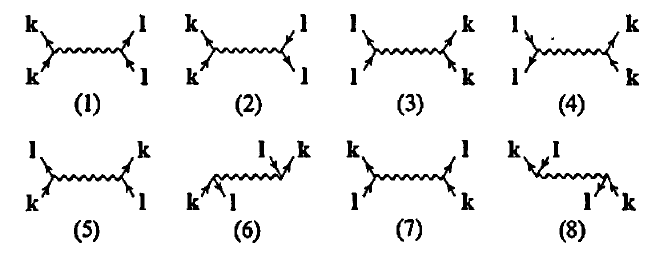
\includegraphics[width=0.8\textwidth]{screenshots/first-order-wiggly.PNG}
\end{equation}
The diagrams such as
\begin{center}
\tikzset{every picture/.style={line width=0.75pt}} %set default line width to 0.75pt        

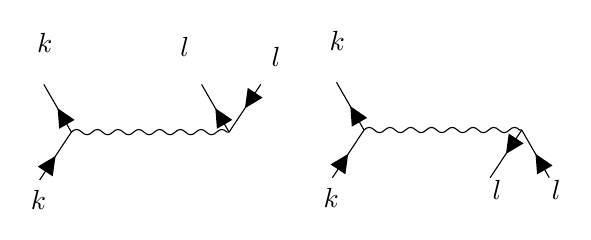
\begin{tikzpicture}[x=0.75pt,y=0.75pt,yscale=-1,xscale=1]
%uncomment if require: \path (0,244); %set diagram left start at 0, and has height of 244

%Straight Lines [id:da9760212638037913] 
\draw    (93.78,111.78) .. controls (95.45,110.11) and (97.11,110.11) .. (98.78,111.78) .. controls (100.45,113.45) and (102.11,113.45) .. (103.78,111.78) .. controls (105.45,110.11) and (107.11,110.11) .. (108.78,111.78) .. controls (110.45,113.45) and (112.11,113.45) .. (113.78,111.78) .. controls (115.45,110.11) and (117.11,110.11) .. (118.78,111.78) .. controls (120.45,113.45) and (122.11,113.45) .. (123.78,111.78) .. controls (125.45,110.11) and (127.11,110.11) .. (128.78,111.78) .. controls (130.45,113.45) and (132.11,113.45) .. (133.78,111.78) .. controls (135.45,110.11) and (137.11,110.11) .. (138.78,111.78) .. controls (140.45,113.45) and (142.11,113.45) .. (143.78,111.78) .. controls (145.45,110.11) and (147.11,110.11) .. (148.78,111.78) .. controls (150.45,113.45) and (152.11,113.45) .. (153.78,111.78) .. controls (155.45,110.11) and (157.11,110.11) .. (158.78,111.78) .. controls (160.45,113.45) and (162.11,113.45) .. (163.78,111.78) .. controls (165.45,110.11) and (167.11,110.11) .. (168.78,111.78) -- (169.78,111.78) -- (169.78,111.78) ;
%Straight Lines [id:da4571267837545099] 
\draw    (80.53,88.8) -- (93.78,111.78) ;
\draw [shift={(87.16,100.29)}, rotate = 60.03] [fill={rgb, 255:red, 0; green, 0; blue, 0 }  ][line width=0.08]  [draw opacity=0] (8.93,-4.29) -- (0,0) -- (8.93,4.29) -- cycle    ;
%Straight Lines [id:da08135471840003439] 
\draw    (93.78,111.78) -- (78.53,134.8) ;
\draw [shift={(86.16,123.29)}, rotate = 123.53] [fill={rgb, 255:red, 0; green, 0; blue, 0 }  ][line width=0.08]  [draw opacity=0] (8.93,-4.29) -- (0,0) -- (8.93,4.29) -- cycle    ;
%Straight Lines [id:da42744127070386173] 
\draw    (185.04,88.76) -- (169.78,111.78) ;
\draw [shift={(177.41,100.27)}, rotate = 303.53] [fill={rgb, 255:red, 0; green, 0; blue, 0 }  ][line width=0.08]  [draw opacity=0] (8.93,-4.29) -- (0,0) -- (8.93,4.29) -- cycle    ;
%Straight Lines [id:da3731869684683673] 
\draw    (156.53,88.8) -- (169.78,111.78) ;
\draw [shift={(163.16,100.29)}, rotate = 60.03] [fill={rgb, 255:red, 0; green, 0; blue, 0 }  ][line width=0.08]  [draw opacity=0] (8.93,-4.29) -- (0,0) -- (8.93,4.29) -- cycle    ;
%Straight Lines [id:da9023180120241947] 
\draw    (234.78,110.78) .. controls (236.45,109.11) and (238.11,109.11) .. (239.78,110.78) .. controls (241.45,112.45) and (243.11,112.45) .. (244.78,110.78) .. controls (246.45,109.11) and (248.11,109.11) .. (249.78,110.78) .. controls (251.45,112.45) and (253.11,112.45) .. (254.78,110.78) .. controls (256.45,109.11) and (258.11,109.11) .. (259.78,110.78) .. controls (261.45,112.45) and (263.11,112.45) .. (264.78,110.78) .. controls (266.45,109.11) and (268.11,109.11) .. (269.78,110.78) .. controls (271.45,112.45) and (273.11,112.45) .. (274.78,110.78) .. controls (276.45,109.11) and (278.11,109.11) .. (279.78,110.78) .. controls (281.45,112.45) and (283.11,112.45) .. (284.78,110.78) .. controls (286.45,109.11) and (288.11,109.11) .. (289.78,110.78) .. controls (291.45,112.45) and (293.11,112.45) .. (294.78,110.78) .. controls (296.45,109.11) and (298.11,109.11) .. (299.78,110.78) .. controls (301.45,112.45) and (303.11,112.45) .. (304.78,110.78) .. controls (306.45,109.11) and (308.11,109.11) .. (309.78,110.78) -- (310.78,110.78) -- (310.78,110.78) ;
%Straight Lines [id:da768308410681679] 
\draw    (221.53,87.8) -- (234.78,110.78) ;
\draw [shift={(228.16,99.29)}, rotate = 60.03] [fill={rgb, 255:red, 0; green, 0; blue, 0 }  ][line width=0.08]  [draw opacity=0] (8.93,-4.29) -- (0,0) -- (8.93,4.29) -- cycle    ;
%Straight Lines [id:da7130025901944149] 
\draw    (234.78,110.78) -- (219.53,133.8) ;
\draw [shift={(227.16,122.29)}, rotate = 123.53] [fill={rgb, 255:red, 0; green, 0; blue, 0 }  ][line width=0.08]  [draw opacity=0] (8.93,-4.29) -- (0,0) -- (8.93,4.29) -- cycle    ;
%Straight Lines [id:da8657016622612258] 
\draw    (310.78,110.78) -- (295.53,133.8) ;
\draw [shift={(303.16,122.29)}, rotate = 303.53] [fill={rgb, 255:red, 0; green, 0; blue, 0 }  ][line width=0.08]  [draw opacity=0] (8.93,-4.29) -- (0,0) -- (8.93,4.29) -- cycle    ;
%Straight Lines [id:da9413606756365827] 
\draw    (310.78,110.78) -- (324.04,133.76) ;
\draw [shift={(317.41,122.27)}, rotate = 60.03] [fill={rgb, 255:red, 0; green, 0; blue, 0 }  ][line width=0.08]  [draw opacity=0] (8.93,-4.29) -- (0,0) -- (8.93,4.29) -- cycle    ;

% Text Node
\draw (76,62.73) node [anchor=north west][inner sep=0.75pt]    {$k$};
% Text Node
\draw (73,138.73) node [anchor=north west][inner sep=0.75pt]    {$k$};
% Text Node
\draw (189,69.73) node [anchor=north west][inner sep=0.75pt]    {$l$};
% Text Node
\draw (145,64.73) node [anchor=north west][inner sep=0.75pt]    {$l$};
% Text Node
\draw (217,61.73) node [anchor=north west][inner sep=0.75pt]    {$k$};
% Text Node
\draw (214,137.73) node [anchor=north west][inner sep=0.75pt]    {$k$};
% Text Node
\draw (324.04,133.76) node [anchor=north west][inner sep=0.75pt]    {$l$};
% Text Node
\draw (295.53,133.8) node [anchor=north west][inner sep=0.75pt]    {$l$};


\end{tikzpicture}
\end{center}
are \bluep{not allowed since they have a particle and a hole in the same state $\mathbf{l}$.} It can be shown that diagrams (1),(3),(5) and (7) above do not occur either. The term in disturbed Hamiltonian that corresponds to (1) is 
\begin{equation}
    V_{klkl}a^{\dagger}_ka^{\dagger}_la_ka_l
\end{equation}
when this acts on the state with one incoming particle in $\phi_k$, we find
$$V_{k l k l} a_{k}^{\dagger} a_{l}^{\dagger} a_{k} a_{l}|1^p_k\rangle=0$$
Diagrams (3),(5), and (7) are similarly eliminated. Note that the term in $H_1$ corresponding to diagram (2) is (following the rule of left-out,right-out, left-in,right-in):
\begin{equation}V_{k l k l} a_{k}^{\dagger}b_l a_{k} b_{l}^{\dagger}\end{equation}
and
\begin{equation}V_{k l k l}  a_{k}^{\dagger}b_{l} a_{k} b_{l}^{\dagger}\left|1_{k}^{p}\right\rangle=V_{k l k l}\left|1_{k}^{p}\right\rangle \neq 0\end{equation}
The possible first-order processes may then be drawn using (2),(4),(6),(8). \textbf{This can only be done in one way, e.g., by in each case attaching the outgoing $\mathbf{l}$ line to the incoming one. Thus we find:}
\begin{equation}
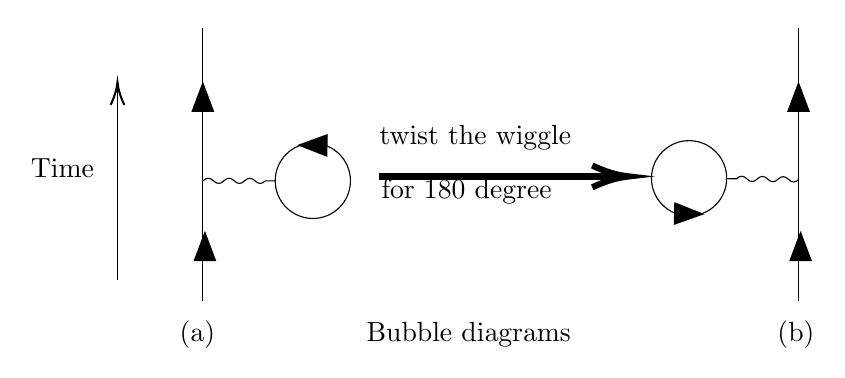
\begin{tikzpicture}[x=0.75pt,y=0.75pt,yscale=-1,xscale=1]
%uncomment if require: \path (0,235); %set diagram left start at 0, and has height of 235

%Straight Lines [id:da10068577398388545] 
\draw    (172,46.6) -- (172,178) ;
%Shape: Triangle [id:dp19925235312138345] 
\draw  [fill={rgb, 255:red, 0; green, 0; blue, 0 }  ,fill opacity=1 ] (172.13,73) -- (177.25,86.6) -- (167,86.6) -- cycle ;
%Shape: Triangle [id:dp004394430560968221] 
\draw  [fill={rgb, 255:red, 0; green, 0; blue, 0 }  ,fill opacity=1 ] (173.13,145) -- (178.25,158.6) -- (168,158.6) -- cycle ;
%Shape: Circle [id:dp41514745661808317] 
\draw   (207,120.13) .. controls (207,110.11) and (215.11,102) .. (225.13,102) .. controls (235.14,102) and (243.25,110.11) .. (243.25,120.13) .. controls (243.25,130.14) and (235.14,138.25) .. (225.13,138.25) .. controls (215.11,138.25) and (207,130.14) .. (207,120.13) -- cycle ;
%Straight Lines [id:da9922958867186198] 
\draw    (172.25,120.13) .. controls (173.92,118.46) and (175.58,118.46) .. (177.25,120.13) .. controls (178.92,121.8) and (180.58,121.8) .. (182.25,120.13) .. controls (183.92,118.46) and (185.58,118.46) .. (187.25,120.13) .. controls (188.92,121.8) and (190.58,121.8) .. (192.25,120.13) .. controls (193.92,118.46) and (195.58,118.46) .. (197.25,120.13) .. controls (198.92,121.8) and (200.58,121.8) .. (202.25,120.13) -- (207,120.13) -- (207,120.13) ;
%Shape: Triangle [id:dp2263151698703949] 
\draw  [fill={rgb, 255:red, 0; green, 0; blue, 0 }  ,fill opacity=1 ] (218.33,102.93) -- (231.98,97.95) -- (231.87,108.19) -- cycle ;
%Straight Lines [id:da3409503459639508] 
\draw    (459,46.6) -- (459,178) ;
%Shape: Triangle [id:dp7202483298889484] 
\draw  [fill={rgb, 255:red, 0; green, 0; blue, 0 }  ,fill opacity=1 ] (459.13,73) -- (464.25,86.6) -- (454,86.6) -- cycle ;
%Shape: Triangle [id:dp05921608545174617] 
\draw  [fill={rgb, 255:red, 0; green, 0; blue, 0 }  ,fill opacity=1 ] (460.13,145) -- (465.25,158.6) -- (455,158.6) -- cycle ;
%Shape: Circle [id:dp43994714997441664] 
\draw   (424.52,119.08) .. controls (424.42,129.09) and (416.22,137.12) .. (406.21,137.01) .. controls (396.2,136.91) and (388.17,128.71) .. (388.27,118.7) .. controls (388.38,108.69) and (396.58,100.66) .. (406.59,100.76) .. controls (416.6,100.87) and (424.63,109.07) .. (424.52,119.08) -- cycle ;
%Straight Lines [id:da8513266846637301] 
\draw    (459.27,119.44) .. controls (457.58,121.09) and (455.92,121.08) .. (454.27,119.39) .. controls (452.62,117.71) and (450.95,117.69) .. (449.27,119.34) .. controls (447.59,120.99) and (445.92,120.97) .. (444.27,119.29) .. controls (442.62,117.6) and (440.96,117.58) .. (439.27,119.23) .. controls (437.59,120.88) and (435.92,120.86) .. (434.27,119.18) .. controls (432.62,117.5) and (430.95,117.48) .. (429.27,119.13) -- (424.52,119.08) -- (424.52,119.08) ;
%Shape: Triangle [id:dp20595976463490984] 
\draw  [fill={rgb, 255:red, 0; green, 0; blue, 0 }  ,fill opacity=1 ] (413.02,136.15) -- (399.31,141) -- (399.53,130.75) -- cycle ;
%Straight Lines [id:da9038937323503633] 
\draw [line width=2.25]    (257,118) -- (373.25,118) ;
\draw [shift={(377.25,118)}, rotate = 180] [color={rgb, 255:red, 0; green, 0; blue, 0 }  ][line width=2.25]    (17.49,-5.26) .. controls (11.12,-2.23) and (5.29,-0.48) .. (0,0) .. controls (5.29,0.48) and (11.12,2.23) .. (17.49,5.26)   ;
%Straight Lines [id:da5407884786763255] 
\draw    (131,168) -- (131,74.6) ;
\draw [shift={(131,72.6)}, rotate = 450] [color={rgb, 255:red, 0; green, 0; blue, 0 }  ][line width=0.75]    (10.93,-3.29) .. controls (6.95,-1.4) and (3.31,-0.3) .. (0,0) .. controls (3.31,0.3) and (6.95,1.4) .. (10.93,3.29)   ;

% Text Node
\draw (256,92) node [anchor=north west][inner sep=0.75pt]   [align=left] {twist the wiggle};
% Text Node
\draw (257,118) node [anchor=north west][inner sep=0.75pt]   [align=left] {for 180 degree};
% Text Node
\draw (88,108) node [anchor=north west][inner sep=0.75pt]   [align=left] {Time};
% Text Node
\draw (159.73,186.07) node [anchor=north west][inner sep=0.75pt]   [align=left] {(a)};
% Text Node
\draw (447.73,186.07) node [anchor=north west][inner sep=0.75pt]   [align=left] {(b)};
% Text Node
\draw (249.73,187.07) node [anchor=north west][inner sep=0.75pt]   [align=left] {Bubble diagrams};


\end{tikzpicture}
\label{bubble-diagrams}
\end{equation}
\begin{equation}
    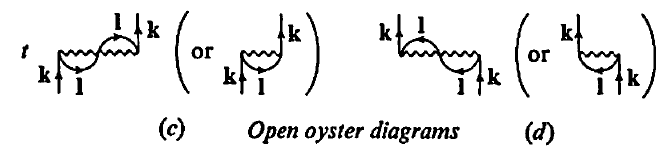
\includegraphics[width=0.8\textwidth]{screenshots/open-oyster-diagrams.PNG}
    \label{open-oyster-diagrams}
\end{equation}
The bubble processes can be physically interpreted as follows: a particle enters in $\mathbf{k}>k_F$, knocks a particle out of state $\mathbf{l}<k_F$ at time t, then knocks the particle instantaneously back into $\mathbf{l}$ at time t, then continues freely in state $\mathbf{k}$.

The open-oyster processes are just like the bubbles, except that a quick change act occurs in which at time $t$ the incoming particle simultaneously
(a) strikes the particle in $\mathbf{l},(b)$ creates an instantaneous hole in $\mathbf{l}$ and $(c)$ is exchanged for the particle in $\mathbf{l}.$ Diagrams \ref{open-oyster-diagrams}) are often called "first-order exchange diagrams', and the process is referred to as an \textbf{"exchange scattering"}. The instantaneous hole lines in the bubble and open oyster are called \textbf{"non-propagating"} lines.

We now see how to evaluate these diagrams. Consider \ref{bubble-diagrams}(a), we have
\begin{equation}\begin{array}{l}
G^+(\mathbf{k},t_2-t_1)=(-1) \sum_{l<k_{F}} \int_{-\infty}^{+\infty} d t\left[i G_{0}^{+}\left(\mathbf{k}, t-t_{1}\right)\right] \times\left[-\frac{i}{2} V_{k l k l}\right] \times \\
\quad \times\left[i G_{0}^{-}(l, t-t)\right] \times\left[i G_{0}^{+}\left(\mathbf{k}, t_{2}-t\right)\right]
\end{array}\end{equation}
\redp{The extra factor of (-1) in front comes from the fact that the diagram contains one \textbf{"fermion loop"}.} Note that an additional factor of (-1) appears because the propagator line for the bubble is:
\begin{equation}i G_{0}^{-}(1, t-t)=i \times i e^{-i\epsilon_l \times 0}=-1\end{equation}
The Fourier transform is then
\begin{equation}
G^+(\mathbf{k},\omega)=(-1)\left[i G_{0}^{+}(\mathbf{k}, \omega)\right]^{2} \sum_{i<k_{r}}\left[-\frac{i}{2} V_{k l k l}\right](-1)\end{equation}
In a similar fashion, \ref{bubble-diagrams}(b) is
\begin{equation}(-1)\left[i G^+(\mathbf{k},\omega)=G_{0}(\mathbf{k}, \omega)\right]^{2} \sum_{l<k_{r}}\left(-\frac{i}{2}\right) V_{l k l k}(-1)\end{equation}
Since $V_{klkl}=V_{lklk}$ these diagrams are equivalent. From here, we have the following rule:
\begin{imp}
If we are given a diagram, and form a new diagram from it by twisting one or more of its interaction wiggles through 180 degrees, then the new diagram has the same value as the original one. Hence all twisted diagrams may be omitted if we just multiply a correct factor in front.
\end{imp}
In a manner similar to the bubble diagram calculation, the open oyser gives
\begin{equation}
    G^+(\mathbf{k},\omega)=[iG^+_0(\mathbf{k},\omega)]^2\sum_{l<k_F}(-i)V_{lkkl}(-1)
\end{equation}
where the factor of 2 is included, and (-1) comes from $G^{-}_0(\mathbf{k},t-t)$. Observe that the frequency, $\omega$, associated with the propagator line coming out of the interaction is the same as that entering. This is an illustration of "\textbf{conservation of frequency}", and it is a result from the fact that \redp{the Hamiltonian is time-dependent.}

We now summarize the dictionary for the expansion series
\begin{figure}
    \centering
    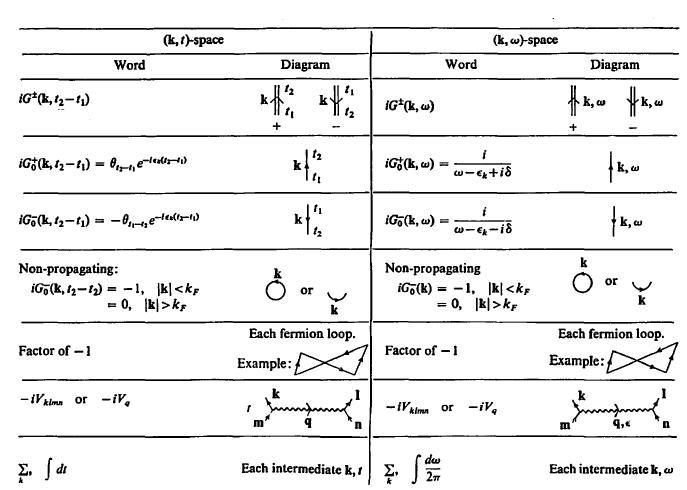
\includegraphics[width=0.8\textwidth]{screenshots/interacting-fermi-sys-dict.PNG}
    \caption{Diagram dictionary for interacting many-fermion system with no external potential (Goldstone method)}
    \label{fig:goldstone-interacting-fermi-dict}
\end{figure}
The diagrams may also be interpreted physically from a particular time $t_0$:
\begin{center}
    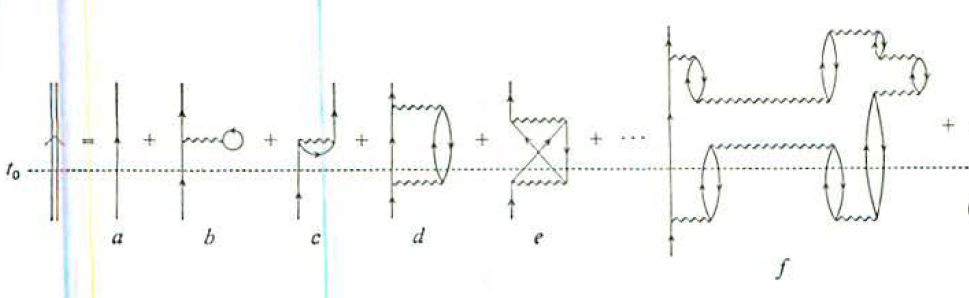
\includegraphics[width=0.8\textwidth]{screenshots/goldstone-particular-time.PNG}
\end{center}
At $t_{0}$ we see that besides the bare particle, there may exist in the many-body system two "virtual' particles plus one hole created by second-order process $d$ or two particles and a hole created by second-order sequence $e,$ and so on, with the particle plus three particle-hole pairs created during the eighth-order poodle process illustrating a typical higher-order case. That is, \textbf{the diagrams show all the particles and holes which may be kicked up by the bare particle as it churns through the Fermi sea.}
\subsection{The "quasi-physical" nature of Feynman diagrams}   
\newpage
\section{Ground State Energy and Vacuum Amplitude}
\subsection{Meaning of the vacuum amplitude}
One of the first many-body problems to be tackled by the field theoretical diagram techniques was that of finding the ground state energy $E_0$ of a system of interacting fermions. The diagrammatic methods in this chapter provide a neat way of handling nuclear and electron interactions. In both cases, we can perform a partial sum over an infinite series of infinite terms and get a finite result. In order to do this, it is necessary to have a general way of writing down the nth-order term in the ordinary perturbation series for $E_0$,i.e., in
\begin{equation}E_{0}=W_{0}+\left\langle\Phi_{0}\left|H_{1}\right| \Phi_{0}\right\rangle+\sum_{m \neq 0} \frac{\left\langle\Phi_{0}\left|H_{1}\right| \phi_{m}\right\rangle\left\langle\Phi_{m}\left|H_{1}\right| \Phi_{0}\right\rangle}{W_{0}-W_{m}}+\cdots
\label{time-indep-ground}
\end{equation}
\textbf{where $W_{0}, W_{m}$ are the ground and excited state energies of the unperturbed Hamiltonian, and $\Phi_{0}, \Phi_{m}$ are the corresponding wave functions. The general term is hard to obtain from the time-independent theory usually used to get (\ref{time-indep-ground}).} However, there is a time-dependent technique which gives a pictorial recipe for finding the desired nth-order term:\redp{\textbf{vacuum amplitude expansion.}}
\begin{imp}
The vacuum amplitude, $R(t),$ is defined as follows: Let $\Phi_{0}$ be the ground state of the unperturbed system (i.e., $\Phi_{0}$ is the \textbf{'Fermi vacuum'}). Then $R(t)$ is the probability amplitude that if the system is in $\Phi_{0}$ at time $0,$ and the external potential and/or interactions between particles are allowed to act, then the system will be in $\Phi_{0}$ at time $t .$ That is, $R(t)$ is the \textbf{\redp{'Fermi vacuum to Fermi vacuum transition amplitude'}}. $R(t)$ can also be called \textbf{"no-particle propagator"}.
\end{imp}
If there is no interaction, then the wave function at time $t$ will simply be $\Phi_0e^{-iW_0t}$ where $W_0$ is the ground state energy. If the interaction is now switched on at time $t=0$, the system will start to make transition from $\Phi_0$ to all possible N-particle states. Let the state after time $t$ be $\Psi(t)$, \bluep{\textbf{this must be obtainable fro m the ground state $\Phi_0$, by some sort of operation.}} Thus:
\begin{equation}\Psi(t)=U(t) \Phi_{0}\end{equation}
which may be regarded as the equation defining the \textbf{"time development operator"},$U(t)$. The probability amplitude $R(t)$ is thus:
\begin{imp}
\begin{equation}\begin{aligned}
R(t) &=\left(\Phi_{0} e^{-i W_{0} t}, \Psi(t)\right)=\int \Phi_{0}^{*} e^{+i W_{0} t} U(t) \Phi_{0} d \mathbf{r}_{1} \dots d \mathbf{r}_{N} \\
& \equiv\left\langle\Phi_{0}|U(t)| \Phi_{0}\right\rangle e^{+i W_{0} t}=\text { vacuum amplitude. }
\end{aligned}
\label{vac-amp-def}
\end{equation}
The importance of the vacuum amplitude lies in the fact that the ground state energy, $E_{0}$, may be obtained from it with the aid of the theorem
\begin{equation}E_{0}=W_{0}+\lim _{t \rightarrow \infty(1-i \eta)} i \frac{d}{d t} \ln R(t)
\label{ground-energy-theorem}
\end{equation}
where $\eta$ is an infinitesimal. Thus, if we can get a diagrammatic expansion of $R(t)$, then the diagram series for $E_0$ follows from \ref{ground-energy-theorem}.
\end{imp}
\begin{mybox}
The diagrammatic perturbation expansion of $R(t)$ is considerably more complicated because of the \textbf{"unlinked" diagrams (i.e. not all vertices are connected).} Lukily, the Logarithm of R turns out to be the sume over just \textbf{"linked diagrams"}. This is the famous \textbf{"linked cluster theorem"}.
\end{mybox}

\subsection{Quantum vacuum amplitude for one-particle system}
Consider the simplest situation first: a Fermi system consisting of one particle in an external potential, with non-degenerate energy levels-for example, an electron in a one-dimensional harmonic oscillator potential. Let the unperturbed Hamiltonian be
$$H_{0}=\frac{p^{2}}{2 m}+U(r)$$
with eigensolutions $\phi_k$,$\epsilon_k$. \bluep{The grpund state of the system consist of one particle in $\phi_1$ and no particles in any higher states;} in occupation number formalism this is $\Phi_0=|1_1,0_2,0_3,\ldots\rangle$. The corresponding ground state is just $W_0=\epsilon_1$. A typical excited state is one particle in $\phi_{k}$ and no particle in any other state: $\Phi_{\text {excited }}=\left|0_{1}, 0_{2}, \ldots, 1_{k}, \ldots\right\rangle .$ In particle-hole notation, the ground state is $\left.\Phi_{0}=|0\right\rangle,$ while a typical excited state consists of a hole in $\phi_{1}$ and a particle in $\phi_{k}: \Phi_{\text {exe }}=\left|1_{1}^{h}, 1_{k}^p\right\rangle .$ Note that in this one-particle system, there is only one possible hole state, e.g., $\phi_{1}$.

Suppose now a perturbation $V(\mathbf{r})$ is added to $H_{0} .$ The vacuum amplitude in that case is the probability amplitude that if the system starts in its ground state $\Phi_{0}$ at $t=0,$ and is acted upon zero or more times by $V(\mathrm{r}),$ then it will be in $\Phi_{0} e^{-iW_{0} t}$ at time $t .$ By analogy with the pinball case, $R(t)$ will be the sum of the probability amplitudes for all the different ways the system can start out in $\Phi_0$, interact with $V(\mathbf{r})$ arbitrary times and return to $\Phi_0$. \textbf{In the zeroth-order process, nothing at all happens as illustrated below:}
\begin{equation}
    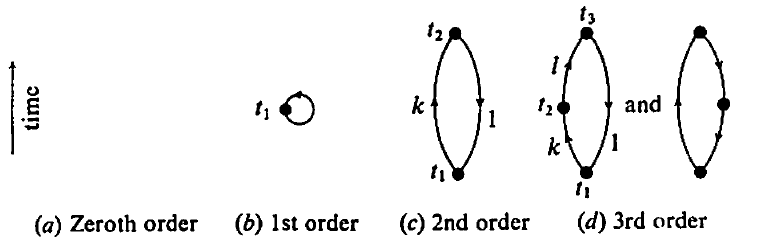
\includegraphics[width=0.8\textwidth]{screenshots/single-electron-diagram-order.PNG}
    \label{single-electron-diagram-order}
\end{equation}
In second order, at $t_1$, $V(\mathbf{t})$ can scatter the particle up into the state $\phi_k$, thus simultaneously creating a hole in $\phi_1$ and a particle in $\phi_k$, and at $t_2$ scatter the particle back into $\phi_1$. The fourth-order ones are
\begin{equation}
    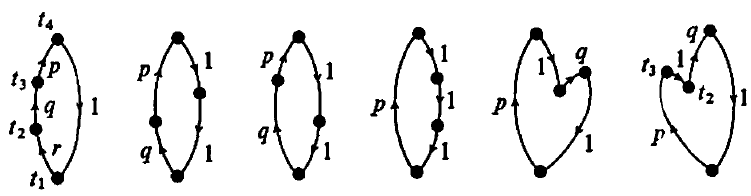
\includegraphics[width=0.8\textwidth]{screenshots/single-electron-4th-order.PNG}
    \label{single-electron-4th-order}
\end{equation}
Note that in the last two diagrams of (\ref{single-electron-4th-order}) there are two particle lines and two hole lines between $t_{2}$ and $t_{3},$ whereas our one-particle system can have at most one particle and one hole. However, it is easily shown that \textbf{these diagrams are exactly cancelled by unlinked diagrams of the sort in (\ref{single-electron-unlinked-diagram}) below}. 
\begin{equation}
    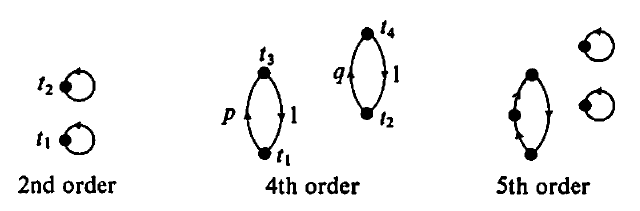
\includegraphics[width=0.8\textwidth]{screenshots/single-electron-unlinked-diagram.PNG}
    \label{single-electron-unlinked-diagram}
\end{equation}
For example, because of \textbf{the (-1) from the extra fermion loop}, the last diagram in (\ref{single-electron-4th-order}) is cancelled by the fourth-order diagram in (\ref{single-electron-unlinked-diagram}). \bluep{Nevertheless, it is necessary to retain such diagrams which violate conservation of particle number, in order to prove the linked cluster theorem.} The same argument holds for diagrams which violate the Pauli exclusion principle.

In order to draw all diagrams in $n$ th order, draw $n$ dots in a vertical row, label them $t_{1}, t_{2}, \ldots, t_{n}$ and connect them up in all possible \textbf{'topologically distinct'} (see below) ways with one line entering and one leaving each dot. For example in third order we find the six diagrams
\begin{center}
    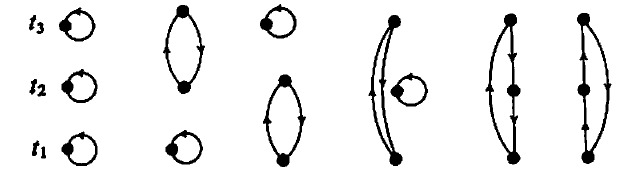
\includegraphics[width=0.8\textwidth]{screenshots/single-electron-topo-distinct.PNG}
\end{center}
Two diagrams are ' \textbf{topologically equivalent}' if one can be \bluep{distorted into the other without changing the vertical ordering of the dots; otherwise they are distinct.} This is illustrated by the fourth-order diagrams (\textbf{note significance of the direction of the arrows}).

Finally, the diagrammatic expansion for the vacuum amplitude will just be the sum of all diagrams such as the above:
\begin{equation}
    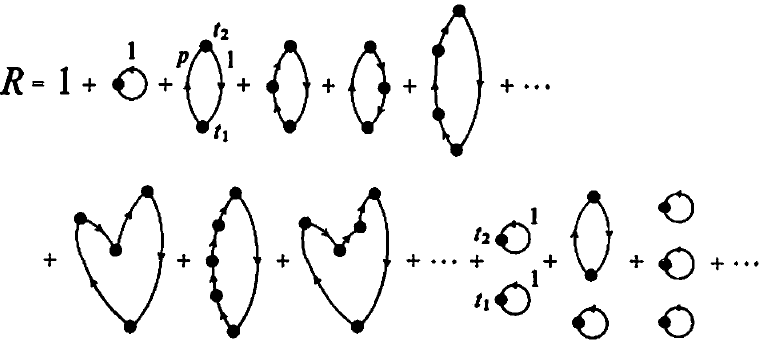
\includegraphics[width=0.8\textwidth]{screenshots/single-electron-ground-expansion.PNG}
    \label{single-electron-ground-expansion}
\end{equation}
where the 1 expresses the fact that in the unperturbed case, the probability amplitude for the system staying in its ground state is 1. Translate the series into equation we have
\begin{equation}
    \begin{aligned}
    R(t)=1-&V_{11} \int_{0}^{t} d t_{1} G_{0}\left(1, t_{1}-t_{1}\right)-\\
    &-\sum_{p>1} V_{1p} V_{p 1} \int_{0}^{t} d t_{1} \int_{0}^{t} \underset{t_2>t_1}{dt_2} G_{0}^{+}\left(p, t_{2}-t_{1}\right) G_{0}^{-}\left(1, t_{1}-t_{2}\right)+\cdots\\
    &+V_{11} V_{11} \int_{0}^{t} d t_{1} \int_{0}^{t} \underset{t_2>t_1}{d t_{2}} \quad G_{0}^{-}\left(1, t_{1}-t_{1}\right) \sigma_{0}\left(1, t_{2}-t_{2}\right)+\cdots
    \end{aligned}
\end{equation}

\subsection{Linked cluster theorem for one-particle system}
The theorem states that
\begin{equation}
    lnR(t)=\Sigma\text{ all linked graphs}
    \label{single-electron-linked-theorem}
\end{equation}
The proof is based on the fact that \textbf{the contribution from a unlinked diagram is proportional to the product of the contribution of its various parts.} Consider for example the $V_{11}V_{11}$ term:
\begin{center}
\tikzset{every picture/.style={line width=0.75pt}} %set default line width to 0.75pt        
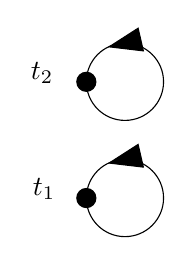
\begin{tikzpicture}[x=0.75pt,y=0.75pt,yscale=-1,xscale=1]
%uncomment if require: \path (0,244); %set diagram left start at 0, and has height of 244

%Shape: Circle [id:dp6498223397318404] 
\draw   (81,85.6) .. controls (81,75.33) and (89.33,67) .. (99.6,67) .. controls (109.87,67) and (118.2,75.33) .. (118.2,85.6) .. controls (118.2,95.87) and (109.87,104.2) .. (99.6,104.2) .. controls (89.33,104.2) and (81,95.87) .. (81,85.6) -- cycle ;
%Shape: Circle [id:dp27995222268876896] 
\draw  [fill={rgb, 255:red, 0; green, 0; blue, 0 }  ,fill opacity=1 ] (76.4,85.6) .. controls (76.4,83.06) and (78.46,81) .. (81,81) .. controls (83.54,81) and (85.6,83.06) .. (85.6,85.6) .. controls (85.6,88.14) and (83.54,90.2) .. (81,90.2) .. controls (78.46,90.2) and (76.4,88.14) .. (76.4,85.6) -- cycle ;
%Shape: Triangle [id:dp3898756772562222] 
\draw  [fill={rgb, 255:red, 0; green, 0; blue, 0 }  ,fill opacity=1 ] (92,68.75) -- (105.94,59.79) -- (108.46,70.7) -- cycle ;
%Shape: Circle [id:dp6531439047197907] 
\draw   (81,141.6) .. controls (81,131.33) and (89.33,123) .. (99.6,123) .. controls (109.87,123) and (118.2,131.33) .. (118.2,141.6) .. controls (118.2,151.87) and (109.87,160.2) .. (99.6,160.2) .. controls (89.33,160.2) and (81,151.87) .. (81,141.6) -- cycle ;
%Shape: Circle [id:dp7775379383850192] 
\draw  [fill={rgb, 255:red, 0; green, 0; blue, 0 }  ,fill opacity=1 ] (76.4,141.6) .. controls (76.4,139.06) and (78.46,137) .. (81,137) .. controls (83.54,137) and (85.6,139.06) .. (85.6,141.6) .. controls (85.6,144.14) and (83.54,146.2) .. (81,146.2) .. controls (78.46,146.2) and (76.4,144.14) .. (76.4,141.6) -- cycle ;
%Shape: Triangle [id:dp43271531457083345] 
\draw  [fill={rgb, 255:red, 0; green, 0; blue, 0 }  ,fill opacity=1 ] (92,124.75) -- (105.94,115.79) -- (108.46,126.7) -- cycle ;

% Text Node
\draw (54,131) node [anchor=north west][inner sep=0.75pt]    {$t_{1}$};
% Text Node
\draw (53,75) node [anchor=north west][inner sep=0.75pt]    {$t_{2}$};
\end{tikzpicture}
\end{center}
Translating it into equation we have
$$
\begin{aligned}
&V_{11} V_{11} \int_{0}^{t} d t_{1} \int_{0}^{t} \underset{t_2>t_1}{d t_{2}} G_{0}^{-} G_{0}^{-}=V_{11}^{2} G_{0}^{-2} \int_{0}^{t} d t_{1} \int_{0}^{t} \underset{t_2>t_1}{d t_{2}}\\
&=V_{11}^{2} G_{0}^{-2} \int_{0}^{t} d t_{1} \int_{0}^{t} d t_{2} \times \frac{1}{2} \quad \text { (where } t_{2}>\text { or }<t_{1})\\
&=\frac{1}{2}\left[V_{11} \int_{0}^{1} d t_{1} G_{0}^{-}\left(1, t_{1}-t_{1}\right)\right] \times\left[V_{11} \int_{0}^{t} d t_{2} G_{0}^{-}\left(1, t_{2}-t_{2}\right)\right]\\
&=\frac{1}{2!}\times\selfcirc^2
\end{aligned}
$$
In general, it turns out that the value of an unlinked diagram with $n$ identical links $L,$ is just $(1 / n !) \times L^{n}$.

A similar factorization occurs for non-identical links if we first sum over all possible time orders. For example, the following three graphs can be summed over:
\begin{center}
\tikzset{every picture/.style={line width=0.75pt}} %set default line width to 0.75pt        
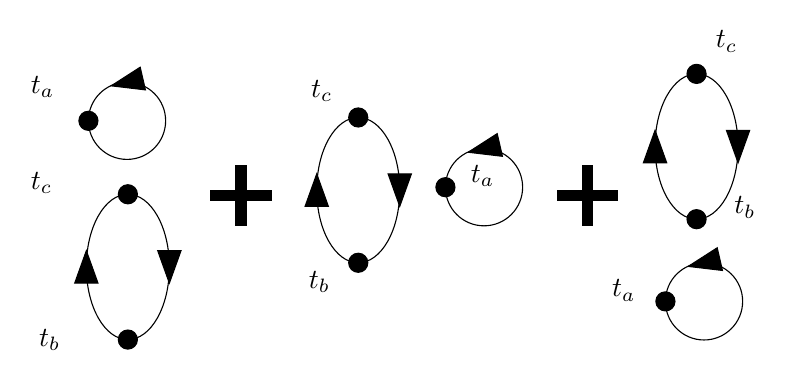
\begin{tikzpicture}[x=0.75pt,y=0.75pt,yscale=-1,xscale=1]
%uncomment if require: \path (0,244); %set diagram left start at 0, and has height of 244

%Shape: Circle [id:dp6498223397318404] 
\draw   (81,85.6) .. controls (81,75.33) and (89.33,67) .. (99.6,67) .. controls (109.87,67) and (118.2,75.33) .. (118.2,85.6) .. controls (118.2,95.87) and (109.87,104.2) .. (99.6,104.2) .. controls (89.33,104.2) and (81,95.87) .. (81,85.6) -- cycle ;
%Shape: Circle [id:dp27995222268876896] 
\draw  [fill={rgb, 255:red, 0; green, 0; blue, 0 }  ,fill opacity=1 ] (76.4,85.6) .. controls (76.4,83.06) and (78.46,81) .. (81,81) .. controls (83.54,81) and (85.6,83.06) .. (85.6,85.6) .. controls (85.6,88.14) and (83.54,90.2) .. (81,90.2) .. controls (78.46,90.2) and (76.4,88.14) .. (76.4,85.6) -- cycle ;
%Shape: Triangle [id:dp3898756772562222] 
\draw  [fill={rgb, 255:red, 0; green, 0; blue, 0 }  ,fill opacity=1 ] (92,68.75) -- (105.94,59.79) -- (108.46,70.7) -- cycle ;
%Shape: Ellipse [id:dp25610156841716825] 
\draw   (100,121) .. controls (111.05,121) and (120,136.67) .. (120,156) .. controls (120,175.33) and (111.05,191) .. (100,191) .. controls (88.95,191) and (80,175.33) .. (80,156) .. controls (80,136.67) and (88.95,121) .. (100,121) -- cycle ;
%Shape: Circle [id:dp9579907217839725] 
\draw  [fill={rgb, 255:red, 0; green, 0; blue, 0 }  ,fill opacity=1 ] (95.4,121) .. controls (95.4,118.46) and (97.46,116.4) .. (100,116.4) .. controls (102.54,116.4) and (104.6,118.46) .. (104.6,121) .. controls (104.6,123.54) and (102.54,125.6) .. (100,125.6) .. controls (97.46,125.6) and (95.4,123.54) .. (95.4,121) -- cycle ;
%Shape: Circle [id:dp44384941541376566] 
\draw  [fill={rgb, 255:red, 0; green, 0; blue, 0 }  ,fill opacity=1 ] (95.4,191) .. controls (95.4,188.46) and (97.46,186.4) .. (100,186.4) .. controls (102.54,186.4) and (104.6,188.46) .. (104.6,191) .. controls (104.6,193.54) and (102.54,195.6) .. (100,195.6) .. controls (97.46,195.6) and (95.4,193.54) .. (95.4,191) -- cycle ;
%Shape: Triangle [id:dp08449835110518966] 
\draw  [fill={rgb, 255:red, 0; green, 0; blue, 0 }  ,fill opacity=1 ] (120,163.8) -- (114.4,148.2) -- (125.6,148.2) -- cycle ;
%Shape: Triangle [id:dp33847857915014856] 
\draw  [fill={rgb, 255:red, 0; green, 0; blue, 0 }  ,fill opacity=1 ] (80,148.2) -- (85.6,163.8) -- (74.4,163.8) -- cycle ;
%Shape: Circle [id:dp16953709843220488] 
\draw   (253,117.6) .. controls (253,107.33) and (261.33,99) .. (271.6,99) .. controls (281.87,99) and (290.2,107.33) .. (290.2,117.6) .. controls (290.2,127.87) and (281.87,136.2) .. (271.6,136.2) .. controls (261.33,136.2) and (253,127.87) .. (253,117.6) -- cycle ;
%Shape: Circle [id:dp23125089891886985] 
\draw  [fill={rgb, 255:red, 0; green, 0; blue, 0 }  ,fill opacity=1 ] (248.4,117.6) .. controls (248.4,115.06) and (250.46,113) .. (253,113) .. controls (255.54,113) and (257.6,115.06) .. (257.6,117.6) .. controls (257.6,120.14) and (255.54,122.2) .. (253,122.2) .. controls (250.46,122.2) and (248.4,120.14) .. (248.4,117.6) -- cycle ;
%Shape: Triangle [id:dp3247983028310686] 
\draw  [fill={rgb, 255:red, 0; green, 0; blue, 0 }  ,fill opacity=1 ] (264,100.75) -- (277.94,91.79) -- (280.46,102.7) -- cycle ;
%Shape: Ellipse [id:dp473301006793975] 
\draw   (211,84) .. controls (222.05,84) and (231,99.67) .. (231,119) .. controls (231,138.33) and (222.05,154) .. (211,154) .. controls (199.95,154) and (191,138.33) .. (191,119) .. controls (191,99.67) and (199.95,84) .. (211,84) -- cycle ;
%Shape: Circle [id:dp7910773789667759] 
\draw  [fill={rgb, 255:red, 0; green, 0; blue, 0 }  ,fill opacity=1 ] (206.4,84) .. controls (206.4,81.46) and (208.46,79.4) .. (211,79.4) .. controls (213.54,79.4) and (215.6,81.46) .. (215.6,84) .. controls (215.6,86.54) and (213.54,88.6) .. (211,88.6) .. controls (208.46,88.6) and (206.4,86.54) .. (206.4,84) -- cycle ;
%Shape: Circle [id:dp29762035839742207] 
\draw  [fill={rgb, 255:red, 0; green, 0; blue, 0 }  ,fill opacity=1 ] (206.4,154) .. controls (206.4,151.46) and (208.46,149.4) .. (211,149.4) .. controls (213.54,149.4) and (215.6,151.46) .. (215.6,154) .. controls (215.6,156.54) and (213.54,158.6) .. (211,158.6) .. controls (208.46,158.6) and (206.4,156.54) .. (206.4,154) -- cycle ;
%Shape: Triangle [id:dp5382643640790852] 
\draw  [fill={rgb, 255:red, 0; green, 0; blue, 0 }  ,fill opacity=1 ] (231,126.8) -- (225.4,111.2) -- (236.6,111.2) -- cycle ;
%Shape: Triangle [id:dp787103954892548] 
\draw  [fill={rgb, 255:red, 0; green, 0; blue, 0 }  ,fill opacity=1 ] (191,111.2) -- (196.6,126.8) -- (185.4,126.8) -- cycle ;
%Shape: Circle [id:dp4980802915672331] 
\draw   (359,172.6) .. controls (359,162.33) and (367.33,154) .. (377.6,154) .. controls (387.87,154) and (396.2,162.33) .. (396.2,172.6) .. controls (396.2,182.87) and (387.87,191.2) .. (377.6,191.2) .. controls (367.33,191.2) and (359,182.87) .. (359,172.6) -- cycle ;
%Shape: Circle [id:dp9401870635500967] 
\draw  [fill={rgb, 255:red, 0; green, 0; blue, 0 }  ,fill opacity=1 ] (354.4,172.6) .. controls (354.4,170.06) and (356.46,168) .. (359,168) .. controls (361.54,168) and (363.6,170.06) .. (363.6,172.6) .. controls (363.6,175.14) and (361.54,177.2) .. (359,177.2) .. controls (356.46,177.2) and (354.4,175.14) .. (354.4,172.6) -- cycle ;
%Shape: Triangle [id:dp7535245748392855] 
\draw  [fill={rgb, 255:red, 0; green, 0; blue, 0 }  ,fill opacity=1 ] (370,155.75) -- (383.94,146.79) -- (386.46,157.7) -- cycle ;
%Shape: Ellipse [id:dp796880375497128] 
\draw   (374,63) .. controls (385.05,63) and (394,78.67) .. (394,98) .. controls (394,117.33) and (385.05,133) .. (374,133) .. controls (362.95,133) and (354,117.33) .. (354,98) .. controls (354,78.67) and (362.95,63) .. (374,63) -- cycle ;
%Shape: Circle [id:dp2607772888080764] 
\draw  [fill={rgb, 255:red, 0; green, 0; blue, 0 }  ,fill opacity=1 ] (369.4,63) .. controls (369.4,60.46) and (371.46,58.4) .. (374,58.4) .. controls (376.54,58.4) and (378.6,60.46) .. (378.6,63) .. controls (378.6,65.54) and (376.54,67.6) .. (374,67.6) .. controls (371.46,67.6) and (369.4,65.54) .. (369.4,63) -- cycle ;
%Shape: Circle [id:dp36338449977521137] 
\draw  [fill={rgb, 255:red, 0; green, 0; blue, 0 }  ,fill opacity=1 ] (369.4,133) .. controls (369.4,130.46) and (371.46,128.4) .. (374,128.4) .. controls (376.54,128.4) and (378.6,130.46) .. (378.6,133) .. controls (378.6,135.54) and (376.54,137.6) .. (374,137.6) .. controls (371.46,137.6) and (369.4,135.54) .. (369.4,133) -- cycle ;
%Shape: Triangle [id:dp6814504901438665] 
\draw  [fill={rgb, 255:red, 0; green, 0; blue, 0 }  ,fill opacity=1 ] (394,105.8) -- (388.4,90.2) -- (399.6,90.2) -- cycle ;
%Shape: Triangle [id:dp44737264879533356] 
\draw  [fill={rgb, 255:red, 0; green, 0; blue, 0 }  ,fill opacity=1 ] (354,90.2) -- (359.6,105.8) -- (348.4,105.8) -- cycle ;
%Shape: Cross [id:dp06220635309920053] 
\draw  [fill={rgb, 255:red, 0; green, 0; blue, 0 }  ,fill opacity=1 ] (152.1,107) -- (156.9,107) -- (156.9,119.1) -- (169,119.1) -- (169,123.9) -- (156.9,123.9) -- (156.9,136) -- (152.1,136) -- (152.1,123.9) -- (140,123.9) -- (140,119.1) -- (152.1,119.1) -- cycle ;
%Shape: Cross [id:dp6139216079282784] 
\draw  [fill={rgb, 255:red, 0; green, 0; blue, 0 }  ,fill opacity=1 ] (319.1,107) -- (323.9,107) -- (323.9,119.1) -- (336,119.1) -- (336,123.9) -- (323.9,123.9) -- (323.9,136) -- (319.1,136) -- (319.1,123.9) -- (307,123.9) -- (307,119.1) -- (319.1,119.1) -- cycle ;

% Text Node
\draw (52,109) node [anchor=north west][inner sep=0.75pt]    {$t_{c}$};
% Text Node
\draw (56,185) node [anchor=north west][inner sep=0.75pt]    {$t_{b}$};
% Text Node
\draw (52,63) node [anchor=north west][inner sep=0.75pt]    {$t_{a}$};
% Text Node
\draw (264,106) node [anchor=north west][inner sep=0.75pt]    {$t_{a}$};
% Text Node
\draw (187,65) node [anchor=north west][inner sep=0.75pt]    {$t_{c}$};
% Text Node
\draw (186,157) node [anchor=north west][inner sep=0.75pt]    {$t_{b}$};
% Text Node
\draw (391,121) node [anchor=north west][inner sep=0.75pt]    {$t_{b}$};
% Text Node
\draw (382,41) node [anchor=north west][inner sep=0.75pt]    {$t_{c}$};
% Text Node
\draw (332,161) node [anchor=north west][inner sep=0.75pt]    {$t_{a}$};


\end{tikzpicture}
\end{center}
Translate into equations we have
\begin{equation}\begin{array}{l}
\sum_{k} V_{k 1} V_{1 k} V_{11} \iiint d t_{a} d t_{b} d t_{c} \times \\
\quad \times G_{0}^{+}\left(k, t_{c}-t_{b}\right) G_{0}^{-}\left(1, t_{b}-t_{c}\right) G_{0}^{-}\left(1, t_{a}-t_{a}\right) x \\
\quad \times\left[\theta_{t_a-t_c}, \theta_{t_c-t_{b}}+\theta_{t_c-t_{a}} \theta_{t_{a}-t_{b}}+\theta_{t_c-t_b} \theta_{t_{b}-t_c}\right]\\
=\selfcirc\times\fermiloop
\end{array}\end{equation}
The $\theta^{\prime} s$ are used as a convenient way of writing the time order in the three diagrams. For $t_{c}>t_{b},$ some concentration shows that the term in brackets $=1$ regardless of where $t_{a}$ lies. This means the integral over $t_{a}$ is independent of that over $t_{b}$ and $t_{c},$ so the triple integral factorizes into two parts producing the result shown.

Combining these results, one finds that R may be written
\begin{equation}
\begin{aligned}
&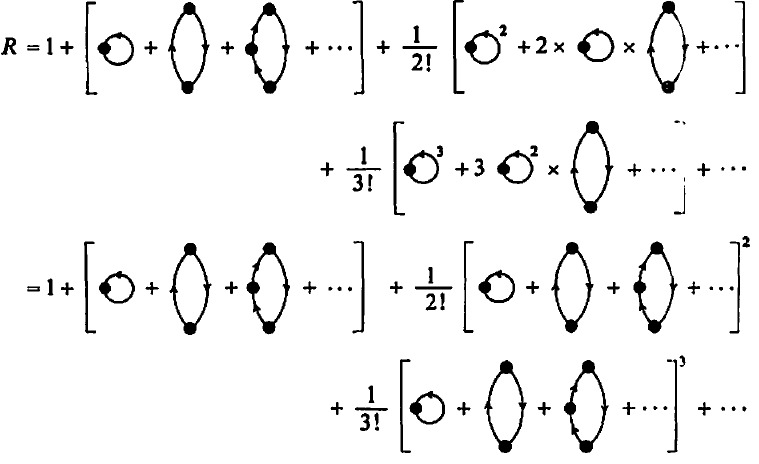
\includegraphics[width=0.8\textwidth]{screenshots/single-electron-R.PNG}\\
&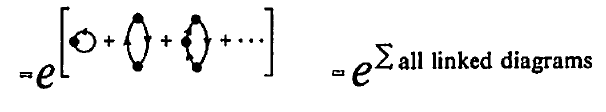
\includegraphics[width=0.8\textwidth]{screenshots/single-electron-R2.PNG}
\end{aligned}
\label{single-electron-R}
\end{equation}
In the many-body case, there is a deeper reason for the importance of the linked cluster theorem, e.g., \bluep{if we do not use it, we find that the perturbation series for the energy appears to diverge badly as the number of particles $N\rightarrow\infty$}.
\subsection{Finding the ground state energy in one-particle system}
Because the ground state energy depends only on the logarithm of $R$:
$$
E_{0}=\epsilon_{1}+\lim _{t \rightarrow \infty(1-i \eta)} i \frac{d}{d t} \ln R(t)
$$
it is now possible to obtain the expression for the ground state energy by translating the above diagrams into the following equations(remember \bluep{the (-1) factor in front of the "limit" is for the "fermion loop"}):
\begin{equation}
    \begin{aligned}
    E_{0}=&\epsilon_{1}-\lim _{n \rightarrow \infty(1-i\eta )} i \frac{d}{d t}\left\{(-i) V_{11} \int_{0}^{t} d t_{1} i G_{0}^{-}\left(1, t_{1}-t_{1}\right)+\right.\\
    &\left.+\sum_{p \neq 1}(-i)^{2} V_{1 p} V_{p 1} \int_{0}^{t} d t_{1} \int_{0}^{t} \underset{t_2>t_1}{d t_{2}} i G_{0}^{+}\left(p, t_{2}-t_{1}\right) i G_{0}^{-}\left(1, t_{1}-t_{2}\right)+\cdots\right\}
    \end{aligned}
\end{equation}
Thus, 
$$
E_0^{(1)}=\lim_{t\rightarrow\infty(1-i\eta)}i\frac{d}{dt}\selfcirc=V_{11}
$$
and the second term produces
$$
\begin{aligned}
\fermiloop&=(-1)^{2}(-i)^{2} \sum_{p \neq 1} V_{1 p} V_{p 1} \int_{0}^{1} d t_{1} \int_{0}^{t} d t_{2} \theta_{t_2-t_1} e^{-i\left(\epsilon_{p}-\epsilon_{1}\right)\left(t_{2}-t_{1}\right)}\\
&=(-1)^{2}(-i)^{2} \sum_{p \neq 1} V_{1 p} V_{p 1} \int_{0}^{t} d t_{1} \int_{0}^{t-t_{1}} d\left(t_{2}-t_{1}\right) e^{-i\left(\epsilon_{p}-\epsilon_1\right)\left(t_{2}-t_{1}\right)}
\end{aligned}
$$
Thus
$$
\lim _{t \rightarrow \infty(1-i\eta)} i \frac{d}{d t}\fermiloop=-i \sum_{p \neq 1} V_{1 p} V_{p 1}\left[-\frac{e^{-i\left(\epsilon_{p}-\epsilon_{1}\right) \omega(1-i \eta)}}{i\left(\epsilon_{p}-\epsilon_{1}\right)}+\frac{1}{i\left(\epsilon_{p}-\epsilon_{1}\right)}\right]
$$
or
\begin{equation}E_{0}^{(2)}=\sum_{p \neq 1} \frac{V_{1 p} V_{p 1}}{\epsilon_{1}-\epsilon_{p}}\end{equation}
where \redp{\textbf{the oscillating exponential is killed because $\left(\epsilon_{1}-\epsilon_{p}\right)$ and the infinitesimal $\eta \text { are both positive. (Note that } \eta \text { is chosen such that } \eta \times \infty=\infty .)$}} Proceeding in this way yields the third-and fourth-order terms:
\begin{equation}E_{0}^{(3)}=\sum_{p, q \neq 1} \frac{V_{1 p} V_{p q} V_{q 1}}{\left(\epsilon_{1}-\epsilon_{p}\right)\left(\epsilon_{1}-\epsilon_{q}\right)}-\sum_{p \neq 1} \frac{V_{1p}V_{p1} V_{11}}{\left(\epsilon_{1}-\epsilon_{p}\right)^{2}}
\label{single-electron-third-order}
\end{equation}
\begin{equation}
\begin{aligned}
E_{0}^{(4)}=& \sum_{p, q, r \neq 1} \frac{V_{1 p} V_{p q} V_{q r} V_{r 1}}{\left(\epsilon_{1}-\epsilon_{p}\right)\left(\epsilon_{1}-\epsilon_{q}\right)\left(\epsilon_{1}-\epsilon_{r}\right)}-\sum_{p, q \neq1} \frac{V_{1p} V_{p q} V_{q 1} V_{11}}{\left(\epsilon_{1}-\epsilon_{p}\right)^{2}\left(\epsilon_{1}-\epsilon_{q}\right)}-\\
&-\sum_{p, q \neq 1} \frac{V_{1 p} V_{p q} V_{q 1} V_{11}}{\left(\epsilon_{1}-\epsilon_{p}\right)\left(\epsilon_{1}-\epsilon_{q}\right)^{2}}+\sum_{p \neq 1} \frac{V_{1p} V_{p 1} V_{11} V_{11}}{\left(\epsilon_{1}-\epsilon_{p}\right)^{3}}-\\
&-\sum_{p, q \neq 1} \frac{V_{1 p} V_{p 1} V_{1 q} V_{q 1}}{\left(\epsilon_{1}-\epsilon_{p}\right)^{2}\left(\epsilon_{1}-\epsilon_{q}\right)}
\end{aligned}
\label{single-electron-fourth-order}
\end{equation}
This is the well-known Rayleigh-Schrodinger perturbation series carried out to fourth order. Now we use diagrammatic method to carry out the calculation to infinite order by \textbf{providing a systematic method for writing out the $nth-$order term in the expansion of $E_0$.}
\begin{imp}
To get the numerator of each term in (\ref{single-electron-third-order}-\ref{single-electron-fourth-order}), the product of $V_{kl}$ factors associated with the interaction dots will do. To get the denominator, draw light dotted horizontal lines \redp{between successive (in time) pairs of vertices}, thus
\begin{center}
    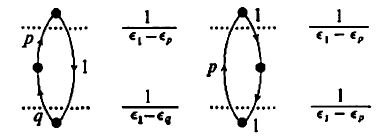
\includegraphics[width=0.8\textwidth]{screenshots/single-electron-denominator-rule.PNG}
\end{center}
and associated a factor of
\begin{equation}
    \frac{1}{\underset{\parbox{100pt}{\centering\tiny{all hole lines intersected by dotted line}}}{\Sigma \epsilon_1}-\underset{\parbox{100pt}{\centering\tiny{all particle lines intersected by dotted line}}}{\Sigma\epsilon_p}}
\end{equation}
The proper sign is obtained by multiplying by the factor $(-1)^{h+1}$ where h=number of hole lines in the diagram. The final rule is to sum over all particle indices.
\end{imp}
Applying these rules (which can be rigorously proved from the vacuum amplitude expansion) yields both of the third-order terms and they also produce the correct result in the other orders. (Note that in fourth order, the last term in (\ref{single-electron-fourth-order}) is obtained by summing the two "mitten" diagrams of (\ref{single-electron-4th-order}).)

Imagine that the perturbing potential is so large that it is impossible to get a decent result by using the usual method of cutting off the series after the first few orders. But suppose, for example, that the potential happens to have big matrix elements only between the ground and first excited states, i.e.,that $V_{12}$ and $V_{21}$ are large but all others are small. Then the perturbation series may be approximated by a partial sum over just those special diagrams in which all vertices connect '1' lines and '2' lines. This means that $E_0$ reduces to a sum over just the following diagrams
\begin{equation}
    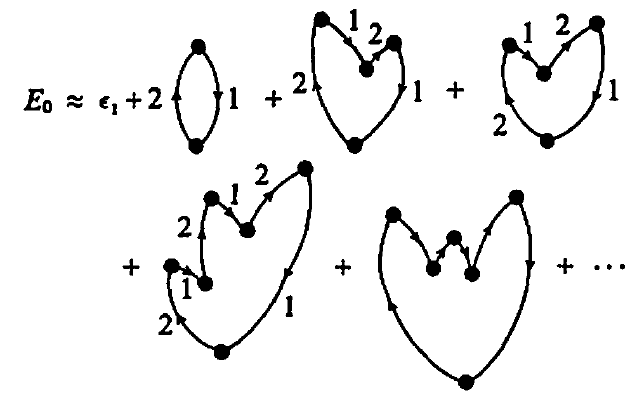
\includegraphics[width=0.8\textwidth]{screenshots/single-electron-V12-series.PNG}
    \label{single-electron-V12-series}
\end{equation}
\bluep{Note that the odd-order diagrams do not occur. And each term representing a graph type is multiplied with a degeneracy factor}. Using the rules this series yields
\begin{equation}\begin{aligned}
E_{0} \approx \epsilon_{1} &+\frac{\left|V_{12}\right|^{2}}{\epsilon_{1}-\epsilon_{2}}-\frac{\left|V_{12}\right|^{4}}{\left(\epsilon_{1}-\epsilon_{2}\right) \times 2\left(\epsilon_{1}-\epsilon_{2}\right) \times\left(\epsilon_{1}-\epsilon_{2}\right)} \times 2 \\
&+\frac{\left|V_{12}\right|^{6}}{\left(\epsilon_{1}-\epsilon_{2}\right) \times 2\left(\epsilon_{1}-\epsilon_{2}\right) \times\left(\epsilon_{1}-\epsilon_{2}\right) \times 2\left(\epsilon_{1}-\epsilon_{2}\right) \times\left(\epsilon_{1}-\epsilon_{2}\right)} \times 4 \\
&+\frac{\left|V_{12}\right|^{6}}{\left(\epsilon_{1}-\epsilon_{2}\right) \times 2\left(\epsilon_{1}-\epsilon_{2}\right) \times 3\left(\epsilon_{1}-\epsilon_{2}\right) \times 2\left(\epsilon_{1}-\epsilon_{2}\right) \times\left(\epsilon_{1}-\epsilon_{2}\right)} \times 12 \\
&+\cdots\\
&=\epsilon_{1}+\frac{\left|V_{12}\right|^{2}}{\epsilon_{1}-\epsilon_{2}}-\frac{\left|V_{12}\right|^{4}}{\left(\epsilon_{1}-\epsilon_{2}\right)^{3}}+\frac{2\left|V_{12}\right|^{6}}{\left(\epsilon_{1}-\epsilon_{2}\right)^{5}}+\cdots
\end{aligned}\end{equation}
\redp{Note that the term $2(\epsilon_1-\epsilon_2)$ comes from the fact that the vertical line intersects with 2 hole lines and 2 particle liens}. By adding and subtracting $\epsilon_{1} / 2$ and factoring out $\frac{1}{2}\left(\epsilon_{1}-\epsilon_{2}\right)$ yielding
\begin{equation}E_{0}=\frac{\epsilon_{1}+\epsilon_{2}}{2}+\frac{\left(\epsilon_{1}-\epsilon_{2}\right)}{2}\left[1+\frac{2\left|V_{12}\right|^{2}}{\left(\epsilon_{1}-\epsilon_{2}\right)^{2}}-\frac{2\left|V_{12}\right|^{4}}{\left(\epsilon_{1}-\epsilon_{2}\right)^{4}}+\frac{4\left|V_{12}\right|^{6}}{\left(\epsilon_{1}-\epsilon_{2}\right)^{6}}+\cdots\right]\end{equation}
The bracketed term is seen to be just the infinite series for the square root, giving us the final result
\begin{equation}E_{0} \approx \frac{\epsilon_{1}+\epsilon_{2}}{2}+\frac{\left(\epsilon_{1}-\epsilon_{2}\right)}{2} \sqrt{\left\{1+\frac{4\left|V_{12}\right|^{2}}{\left(\epsilon_{1}-\epsilon_{2}\right)^{2}}\right\}}\end{equation}
\subsection{The many-body case}
The vacuum amplitude may then be built up as the sum of all possible sequences of interactions beginning and ending in the many-body ground state, or vacuum. The ground state energy again involves just the sum over linked diagrams and may be written as follows:
\begin{equation}
    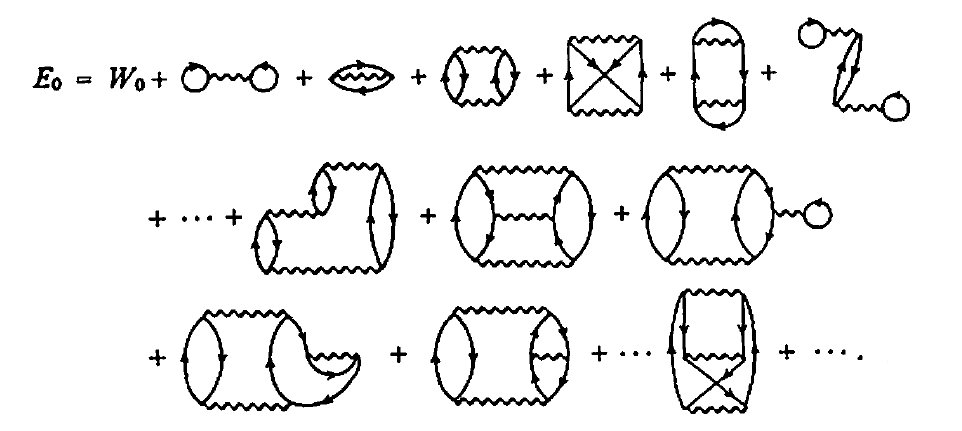
\includegraphics[width=0.8\textwidth]{screenshots/many-body-vacuum-series.PNG}
    \label{many-body-vacuum-series}
\end{equation}
Here we will content ourselves with briefly mentioning a few popular approximations for the ground state energy which can be made with (\ref{many-body-vacuum-series}).

The simplest approximation is the \textbf{\redp{Hartree-Fock (HF), which is just the sum of the double-bubble and oyster diagrams}}:
\begin{equation}
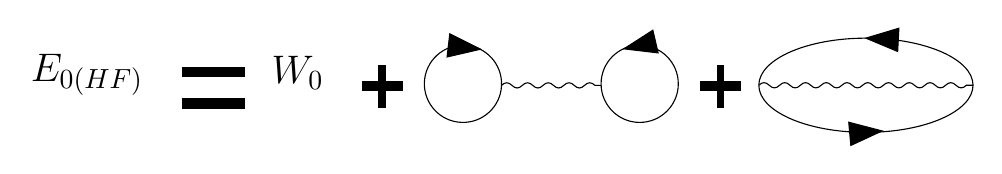
\begin{tikzpicture}[x=0.75pt,y=0.75pt,yscale=-1,xscale=1]
%uncomment if require: \path (0,244); %set diagram left start at 0, and has height of 244

%Shape: Circle [id:dp6498223397318404] 
\draw   (302,124.6) .. controls (302,114.33) and (310.33,106) .. (320.6,106) .. controls (330.87,106) and (339.2,114.33) .. (339.2,124.6) .. controls (339.2,134.87) and (330.87,143.2) .. (320.6,143.2) .. controls (310.33,143.2) and (302,134.87) .. (302,124.6) -- cycle ;
%Shape: Triangle [id:dp3898756772562222] 
\draw  [fill={rgb, 255:red, 0; green, 0; blue, 0 }  ,fill opacity=1 ] (313,107.75) -- (326.94,98.79) -- (329.46,109.7) -- cycle ;
%Shape: Cross [id:dp06220635309920053] 
\draw  [fill={rgb, 255:red, 0; green, 0; blue, 0 }  ,fill opacity=1 ] (195.01,115.6) -- (198.19,115.6) -- (198.19,123.61) -- (206.2,123.61) -- (206.2,127.99) -- (198.19,127.99) -- (198.19,136) -- (195.01,136) -- (195.01,127.99) -- (187,127.99) -- (187,123.61) -- (195.01,123.61) -- cycle ;
%Shape: Circle [id:dp6991360552110061] 
\draw   (216.87,123.85) .. controls (217.28,113.58) and (225.94,105.6) .. (236.2,106.01) .. controls (246.47,106.43) and (254.45,115.08) .. (254.04,125.35) .. controls (253.63,135.61) and (244.97,143.6) .. (234.71,143.18) .. controls (224.44,142.77) and (216.46,134.11) .. (216.87,123.85) -- cycle ;
%Shape: Triangle [id:dp7130261056413152] 
\draw  [fill={rgb, 255:red, 0; green, 0; blue, 0 }  ,fill opacity=1 ] (243.95,107.93) -- (227.8,111.66) -- (229.11,100.54) -- cycle ;
%Straight Lines [id:da10547511660578635] 
\draw    (254.04,125.35) .. controls (255.71,123.68) and (257.37,123.68) .. (259.04,125.35) .. controls (260.71,127.02) and (262.37,127.02) .. (264.04,125.35) .. controls (265.71,123.68) and (267.37,123.68) .. (269.04,125.35) .. controls (270.71,127.02) and (272.37,127.02) .. (274.04,125.35) .. controls (275.71,123.68) and (277.37,123.68) .. (279.04,125.35) .. controls (280.71,127.02) and (282.37,127.02) .. (284.04,125.35) .. controls (285.71,123.68) and (287.37,123.68) .. (289.04,125.35) .. controls (290.71,127.02) and (292.37,127.02) .. (294.04,125.35) .. controls (295.71,123.68) and (297.37,123.68) .. (299.04,125.35) -- (302,125.35) -- (302,125.35) ;
%Shape: Ellipse [id:dp18198799795452325] 
\draw   (378,125.3) .. controls (378,112.76) and (401.1,102.6) .. (429.6,102.6) .. controls (458.1,102.6) and (481.2,112.76) .. (481.2,125.3) .. controls (481.2,137.84) and (458.1,148) .. (429.6,148) .. controls (401.1,148) and (378,137.84) .. (378,125.3) -- cycle ;
%Shape: Triangle [id:dp6530702261537764] 
\draw  [fill={rgb, 255:red, 0; green, 0; blue, 0 }  ,fill opacity=1 ] (429.6,102.6) -- (445.47,97.82) -- (444.89,109.01) -- cycle ;
%Shape: Triangle [id:dp7883771420902802] 
\draw  [fill={rgb, 255:red, 0; green, 0; blue, 0 }  ,fill opacity=1 ] (437.37,147.3) -- (422.33,154.28) -- (421.33,143.12) -- cycle ;
%Straight Lines [id:da8945451528371555] 
\draw    (378,125.3) .. controls (379.67,123.63) and (381.33,123.63) .. (383,125.3) .. controls (384.67,126.97) and (386.33,126.97) .. (388,125.3) .. controls (389.67,123.63) and (391.33,123.63) .. (393,125.3) .. controls (394.67,126.97) and (396.33,126.97) .. (398,125.3) .. controls (399.67,123.63) and (401.33,123.63) .. (403,125.3) .. controls (404.67,126.97) and (406.33,126.97) .. (408,125.3) .. controls (409.67,123.63) and (411.33,123.63) .. (413,125.3) .. controls (414.67,126.97) and (416.33,126.97) .. (418,125.3) .. controls (419.67,123.63) and (421.33,123.63) .. (423,125.3) .. controls (424.67,126.97) and (426.33,126.97) .. (428,125.3) .. controls (429.67,123.63) and (431.33,123.63) .. (433,125.3) .. controls (434.67,126.97) and (436.33,126.97) .. (438,125.3) .. controls (439.67,123.63) and (441.33,123.63) .. (443,125.3) .. controls (444.67,126.97) and (446.33,126.97) .. (448,125.3) .. controls (449.67,123.63) and (451.33,123.63) .. (453,125.3) .. controls (454.67,126.97) and (456.33,126.97) .. (458,125.3) .. controls (459.67,123.63) and (461.33,123.63) .. (463,125.3) .. controls (464.67,126.97) and (466.33,126.97) .. (468,125.3) .. controls (469.67,123.63) and (471.33,123.63) .. (473,125.3) .. controls (474.67,126.97) and (476.33,126.97) .. (478,125.3) -- (481.2,125.3) -- (481.2,125.3) ;
%Shape: Cross [id:dp5950770882977249] 
\draw  [fill={rgb, 255:red, 0; green, 0; blue, 0 }  ,fill opacity=1 ] (358.01,115.6) -- (361.19,115.6) -- (361.19,123.61) -- (369.2,123.61) -- (369.2,127.99) -- (361.19,127.99) -- (361.19,136) -- (358.01,136) -- (358.01,127.99) -- (350,127.99) -- (350,123.61) -- (358.01,123.61) -- cycle ;
%Straight Lines [id:da7229955775391892] 
\draw [line width=3.75]    (100,119) -- (130.2,119) ;
%Straight Lines [id:da17096551384597625] 
\draw [line width=3.75]    (100,134) -- (130.2,134) ;

% Text Node
\draw (142,110) node [anchor=north west][inner sep=0.75pt]  [font=\Large]  {$W_{0}$};
% Text Node
\draw (26,109) node [anchor=north west][inner sep=0.75pt]  [font=\Large]  {$E_{0( HF)}$};


\end{tikzpicture}
\end{equation}
These diagrams involve only three simple rules, so we will evaluate them bere. The rules are: (1) $V_{klmn}$ for each interaction,(2) factor (-1) for each hole line and each fermion loop, and (3) a factor of $\frac{1}{2}$ because the graphs are symmetric. Remembering that all lines are hole lines here, we find
$$E_{0(H F)}=\sum_{k<k_{F}} \epsilon_{k}+\frac{1}{2} \sum_{k, l<k_{F}} V_{k l k l}-\frac{1}{2} \sum_{k ,l<k_{F}} V_{l k k l}$$
The approximation which is good for the high density electron gas (random phase approximation, or 'RPA') involves a partial sum over all 'ring' diagrams in second and higher order:
\begin{equation}
    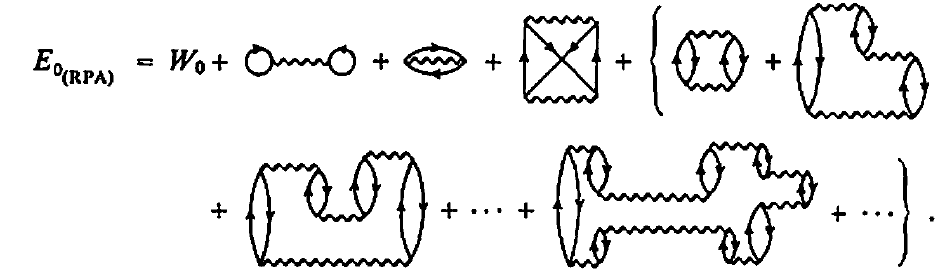
\includegraphics[width=0.8\textwidth]{screenshots/many-body-vacuum-RPA-series.PNG}
\end{equation}
In the case of nuclear matter, we have the 'ladder approximation' involving a partial sum over all ladders:
\begin{equation}
    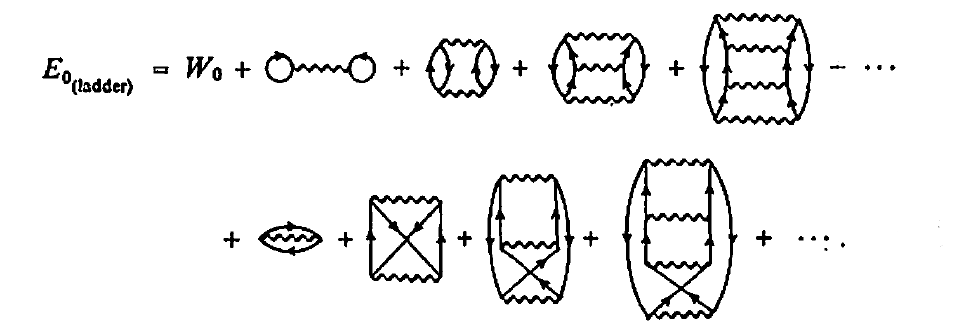
\includegraphics[width=0.8\textwidth]{screenshots/many-body-vacuum-ladder-series.PNG}
\end{equation}
\newpage
\section{Bird's-Eye View of Diagram Methods in the
Many-Body Problem}
\begin{table}[H]
        \centering
        
\begin{tabular}{p{0.45\textwidth}p{0.45\textwidth}}
\hline 
 \begin{center}
Field theoretic ingredient
\end{center}
 & \begin{center}
Significance in many-body theory
\end{center}
 \\
\hline 
 \begin{center}
(1)Occupation number notation
\end{center}
 & \begin{center}
Expresses arbitrary state of manybody system
\end{center}
 \\
\begin{center}
(2)Creation and destruction operators
\end{center}
 & \begin{center}
Primitive operators out of which all many-body operators are built
\end{center}
 \\
\begin{center}
(3)Single particle propagator (Green's function)
\end{center}
 & \begin{center}
Yields quasi particle energies, particle momentum distribution, particle density, ground energy
\end{center}
 \\
\begin{center}
(4)Vacuum amplitude
\end{center}
 & \begin{center}
Gives ground state energy
\end{center}
 \\
\begin{center}
(5)Two-particle Green's function propagator 
\end{center}
 & \begin{center}
Yields energies of collective excitations, electrical conductivity, other non-equilibrium properties
\end{center}
 \\
\begin{center}
(6)Finite temperature vacuum amplitude
\end{center}
 & \begin{center}
Gives equilibrium thermodynamic properties of system
\end{center}
 \\
\begin{center}
(7)Finite temperature propagator
\end{center}
 & \begin{center}
Yields temperature dependence of properties in (3)
\end{center}
 \\

\end{tabular}
        
        \end{table}
\newpage
\section{Occupation Number Formalism (Second Quantization)}
\subsection{Advantages of occupation number formalism}
Since simple things can sometimes get to look pretty formidable in second quantization it is a good idea to understand why many-body physicists all use it. \bluep{The first reason is that it enables us to deal with systems containing a \textbf{variable number of particles}}.It turns out to give an enormous flexibility in the formalism if \textbf{N is allowed to vary in intermediate stages of a calculation and becomes fixed only at the end.} For example, we can put in and remove test particles at will, as in the case of the propagator. Or we can introduce the particle-hole formalism in which the number of particles and holes is variable.

The second reason for the occupation number formalism has to do with the symmetry properties of Fermi and Boss system. Doing things the old
way, we always have to worry about the complicated business of keeping the wave function properly symmetrized. But it turns out that in second quantization, the \textbf{creation and destruction operators obey certain commutation rules which have built into them all the symmetry properties of the system}. By just using these rules we are automatically free from symmetrization headaches.

\subsection{Many-body wave function in occupation number formalism}
Imagine that we are given a system of N identical fermions, which are in general interacting with each other and with an external potential. We have seen that such a system may be described in terms of a set of basis states, $|n_1,...,n_l,...\rangle$ in which the $n_l$ meant $n_l$ particles in the unperturbed single-particle energy eigenstate, $\phi_l$. Actually, \redp{the single-particle states used can be any orthonormal set}. This means that in general, $|n_1,...,n_l,...\rangle$ are not energy eigenstates of either the interacting or the non-interacting system of particles and their choice is determined by convenience. Foe the moment, we will use the $\phi$'s which satisfy the Schrodinger equation:
\begin{equation}\begin{aligned}
H \phi_{k \sigma}(\mathbf{r}, \gamma) &=\epsilon_{k o} \phi_{k o}(\mathbf{r}, \gamma) \\
H=\frac{p^{2}}{2 m}+U(\mathbf{r}) &=-\frac{1}{2 m} \nabla^{2}+U(\mathbf{r}) \\
(\hbar&=1)
\end{aligned}\end{equation}
and $\gamma, \sigma$ are the spin co-ordinate and quantum number respectively. In the case $U(\mathbf{r})=0,$ this has the solutions:
\begin{equation}\begin{aligned}
\phi_{k \sigma}(\mathbf{r}, \gamma) &=\frac{1}{\sqrt{\Omega}} e^{+i \mathbf{k} \cdot \mathbf{r}} \eta_{\sigma}(\gamma) \\
\epsilon_{k} &=\frac{k^{2}}{2 m}(\hbar=1)
\end{aligned}\end{equation}
where $\eta$ is the spin eigenfunction. In general, $\sigma, \gamma$ will be suppressed for brevity, and $\mathbf{k}$ will be short for $\mathbf{k}, \sigma,$ and $\mathbf{r} \equiv \mathbf{r}, \gamma$. 

If there are now N identical non-interacting fermions, the Hamiltonian and Schrodinger equation become
\begin{equation}\begin{array}{c}
H_{0}=\sum_{l=1}^{N} H_{l}, \quad H_{0} \Phi\left(\mathrm{r}_{1}, \ldots, \mathrm{r}_{N}\right)=E \Phi\left(\mathrm{r}_{1}, \ldots, \mathrm{r}_{N}\right) \\
H_{i}=\frac{p^{2}}{2 m}+U\left(\mathrm{r}_{i}\right) ; \quad H_{i} \phi_{k_{i}}=\epsilon_{k_{i}} \phi_{k_{i}}
\end{array}\end{equation}
since the system consists of identical fermions, the wave function must be antisymmetric, i.e., change sign when any two particle co-ordinates are interchanged. This is accomplished by forming a $\Phi$ given by the Slater determinant.
\begin{equation}\Phi_{k_{1} \ldots \ldots k_{N}}\left(\mathrm{r}_{1}, \ldots, \mathrm{r}_{N}\right)=\frac{1}{(N !)^{\frac{1}{2}}} \sum_{P} \gamma_{P} P\left[\phi_{k_{1}}\left(\mathrm{r}_{1}\right) \phi_{k_{2}}\left(\mathrm{r}_{2}\right) \ldots \phi_{k_{N}}\left(\mathrm{r}_{N}\right)\right]\end{equation}
or
\begin{equation}\Phi_{k_{1}, \ldots, k_{N}}\left(\mathbf{r}_{1}, \ldots, \mathbf{r}_{N}\right)=\frac{1}{(N !)^{\frac{1}{2}}}\left|\begin{array}{c}
\phi_{k_{1}}\left(\mathbf{r}_{1}\right) \phi_{k_{1}}\left(\mathbf{r}_{2}\right) \ldots \phi_{k_{1}}\left(\mathbf{r}_{N}\right) \\
\vdots \\
\phi_{k_{N}}\left(\mathbf{r}_{1}\right) \phi_{k_{N}}\left(\mathbf{r}_{2}\right) \dots \phi_{k_{N}}\left(\mathbf{r}_{N}\right)
\end{array}\right|
\label{slater-determinant-2}
\end{equation}
In the first form, $P$ is the permutation operator which interchanges the $\mathbf{r}_{i}$ 's in all possible ways (starting from some standard order), and $\gamma_{P}=-1$ for an odd number of interchanges, and +1 for an even number. The fact that $\Phi=0$ when any two $k_{i}$ 's are equal means that there can't be more than one particle in any state.

A tricky thing about (\ref{slater-determinant-2}) is its sign. For example, in a two-particle system with one particle in state $\phi_{1}$, and the other in $\phi_3$, the wave function is $\Phi_{k_1=1,k_2=3}\equiv\Phi_{13}$ or $\Phi_{k_1=3,k_2=1}\equiv\Phi_{31}$. Since the particles are identical, these represent the same state, but by (\ref{slater-determinant-2}) they differ by a minus sign. To remove this ambiguity, we always write $\Phi$ with the $k$'s in standard order given by:
\begin{equation}\Phi_{k_{1}<k_{2}<\ldots<k_{N}}\end{equation}
A compact way of writing $\Phi$ is
\begin{equation}\begin{aligned}
\Phi_{k_{1}, k_{2}, \ldots, k_{N}}\left(\mathbf{r}_{1}, \mathbf{r}_{2}, \ldots, \mathbf{r}_{N}\right) &=\Phi_{n_{1}, \ldots, n_{i}, \ldots}\left(\mathbf{r}_{1}, \mathbf{r}_{2}, \ldots, \mathbf{r}_{N}\right) \\
&=\left\langle\mathbf{r}_{1}, \mathbf{r}_{2}, \dots, \mathbf{r}_{N} | n_{1}, \dots, n_{i}, \dots\right\rangle
\end{aligned}\end{equation}
It is important to remember that \redp{the $\left|n_{1}, \ldots, n_{1}, \ldots\right\rangle$ are orthogonal and normal because the $\Phi_{k_{1}, \ldots, k_{N}}$ are}, and we may write this in the various equivalent ways
\begin{equation}\begin{array}{l}
\begin{aligned}
&\left\langle n_{1}^{\prime}, n_{2}^{\prime}, \ldots, n_{1}^{\prime}, \ldots | n_{1}, n_{2}, \ldots, n_{1}, \ldots\right\rangle  \\
& \equiv\left(\Phi_{n_{1}^{\prime}, n_{2}^{\prime}\ldots, n_{l}^{\prime}, \ldots} , \Phi_{n_{1}, n_{2}, \ldots, n_{l}, \ldots}\right) \\
& \equiv \int d^{3} \mathbf{r}_{1} \ldots d^{3} \mathbf{r}_{N} \Phi_{n_{1}^{\prime}, n_{2}}^{\prime}, \ldots .\left(\mathbf{r}_{1}, \ldots, \mathbf{r}_{N}\right) \Phi_{n_{1}, n_{2}, \ldots}\left(\mathbf{r}_{1}, \ldots, \mathbf{r}_{N}\right) \\
&=\delta_{n_{1}^{\prime}, n_{1}} \delta_{n_{2}^{\prime}, n_{2}} \ldots \delta_{n_{l}^{\prime}, n_{l}} \cdots .
\end{aligned}
\end{array}\end{equation}
Now we take the step to allow $N$ to be variable, running from 0 to $\infty$. Thus generates the set of basis functions in the following table:
\begin{table}[H]
\caption{Complete set of basis functions used in second quantization}
\centering
\begin{tabular}{ccc}
\hline
N        & $\Phi_{k_1,k_2,...k_N}$                   & $=|n_1,n_2,\ldots,n_i,\ldots\rangle$                                     \\ \hline
0        & $\Phi_0$                                  & $|000\ldots\rangle$                                                      \\
1        & $\Phi_{1}, \Phi_{2}, \Phi_{3}, \ldots$    & $|100 \ldots\rangle,|0100 \ldots\rangle,|00100 \ldots\rangle \ldots$     \\
2        & $\Phi_{12}, \Phi_{13}, \Phi_{23}, \ldots$ & $|1100 \ldots\rangle,|101000 \ldots\rangle,|01100 \ldots\rangle, \ldots$ \\
$\vdots$ & $\vdots$                                  & $\vdots$                                                                
\end{tabular}
\end{table}
This Hilbert space may be pictured as follows:
\begin{equation}
    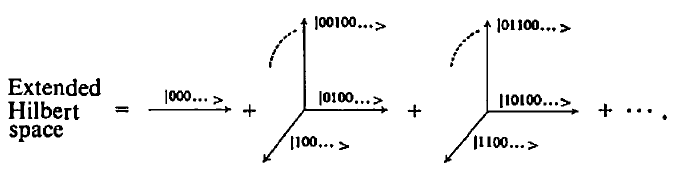
\includegraphics[width=0.8\textwidth]{screenshots/extended-hilbert-space.PNG}
\label{extended-hilbert-space}
\end{equation}

This set is often called 'occupation number basis', and the whole formalism is sometimes referred to as '\redp{occupation number representation}'. Note carefully that we did not get this new basis by unitary transformation (like, for example, is done in going from position to momentum basis).

Only systems of independent fermions without perturbing interactions of any sort have been considered thus far. In the presence of such interactions, \bluep{the $\left.| n_{1}, \ldots, n_{t}, \ldots\right)$ are no longer eigenstates of the total Hamiltonian for the system and the correct eigenstates must be obtained as the linear combination}
\begin{equation}\begin{aligned}
\Psi^{\prime} &=\Phi_{0}+\sum_{k_{1}} A_{k_{1}} \Phi_{k_{1}}+\sum_{k_{1}<k_{2}} A_{k_{1}, k_{2}} \Phi_{k_{1}, k_{2}}+\cdots \\
&=\sum_{n_{1}, \ldots, n_{i}, \ldots} A_{n_{1}, \ldots, n_{i}, \ldots}\left|n_{1}, \ldots, n_{i}, \ldots\right\rangle
\end{aligned}\end{equation}

\subsection{Operators in occupation number formalism}
It was pointed out in Chapter 4 that all operators in this new formalism may be expressed in terms of the creation and destruction operator $c_i^{\dagger}$,$c_i$. The definition of these operators must include a factor of $(\pm1)$ because of antisymmetry. Thus, if $c_i^{\dagger}$,$c_i$ act in such a sequence on the wave function that their net efferct is to exchange two particles, then the wave function must change its sign. Some thought shows that the proper definition is 
\begin{equation}\begin{array}{l}
c_{1}^{\dagger}\left|n_{1}, \ldots, n_{1}, \ldots\right\rangle=(-1)^{\Sigma_{i}}\left(1-n_{i}\right)\left|n_{1}, \ldots, n_{i}+1, \ldots\right\rangle \\
c_{1}\left|n_{1}, \ldots, n_{1}, \ldots\right\rangle=(-1)^{\Sigma_{i}} n_{i}\left|n_{1}, \ldots, n_{i}-1, \ldots\right\rangle
\end{array}\end{equation}
where $\Sigma_i=n_1+n_2+\ldots n_{i-1}$. That is, we get a factor of (-1) for each particle (i.e., each occupied state) standing to the left of the state i in the wave function.

One of the nice properties of the $c_{1}^{\dagger}$ operators is that by applying them repeatedly to the "true vacuum" state (state with no particles in it), it is possible to generate all other states, thus:
\begin{equation}\begin{array}{l}
\Phi_{k_{1}, k_{2}, \ldots, k_{N}}=c_{k_{1}}^{\dagger} c_{k_{2}}^{\dagger} \ldots c_{k_{n}}^{\dagger}|000 \ldots\rangle \\
\left|n_{1}, n_{2}, \ldots\right\rangle=\left(c_{1}\right)^{n_{1}}\left(c_{2}\right)^{n_{2}} \ldots|0000 \ldots\rangle
\end{array}\end{equation}
Another important property of the $c_{1}^{\dagger}, c_{l}$ operators is that they are \redp{\textbf{'hermitian adjoints'}} of each other. This can be seen by constructing matrices for them, using the $\left|n_{1} n_{2}, \ldots, n_{1}, \ldots\right\rangle$ 's as basis states
\begin{equation}
    \begin{aligned}
    &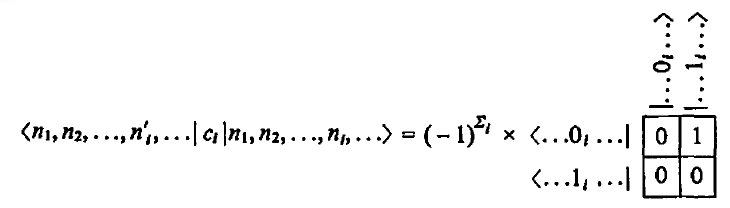
\includegraphics[width=0.8\textwidth]{screenshots/hermitian-adjoint-1.PNG}\\
    &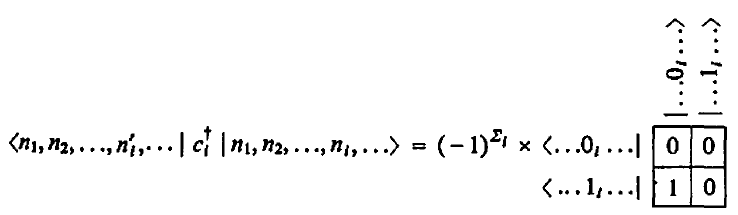
\includegraphics[width=0.8\textwidth]{screenshots/hermitian-adjoint-2.PNG}
    \end{aligned}
\end{equation}
so that
\begin{equation}c_{i}^{\dagger}=\left(c_{i}\right)^{\dagger}\end{equation}
\redp{\textbf{where $\dagger$ means hermitian adjoint. This further shows that $c_{h}^{\dagger} c_{l}$ are nonhermitian and are therefore not observables.}} (otherwise, we should have $c_i=c^{\dagger}_i$). Using the matrices above we can show that:
\begin{equation}\left(c_{i}^{\dagger} c_{i}\right)^{\dagger}=c_{i}^{\dagger} c_{i}\end{equation}
so that $c_i^{\dagger}c_i$ is hermitian. This combination is the famous "\textbf{\redp{number operator}}":
\begin{equation}\hat{n}_{l}=c_{l}^{\dagger} c_{l} ; \quad\left(\hat{N}=\sum_{l} c_{l}^{\dagger} c_{l}\right)\end{equation}
For example
$$c_{i}^{\dagger} c_{i}\left|n_{1}, \dots, n_{i}, \dots\right\rangle=n_{i}\left|n_{1}, \dots, n_{i}, \dots\right\rangle$$

\begin{imp}
The $c_{1}^{\dagger}, c_{1}$ operators obey the following important 'fermion commutation rules':
\begin{equation}
\begin{aligned}
&(1)\left[c_{l}, c_{k}\right]_{+}=c_{l} c_{k}^{\dagger}+c_{k}^{\dagger} c_{l}=\delta_{l k}\\
&(2)\left[c_{l}, c_{k}\right]_{+}=0\\
&(3)\left[c_{l}^{\dagger}, c_{k}^{\dagger}\right]_{+}=0
\end{aligned}
\label{anti-cmmutation-rules-c}
\end{equation}
\end{imp}
These can be easily proved from the definitions:
$$\begin{aligned}
c_{1} c_{k}\left|n_{1}, \ldots, n_{1}, \ldots, n_{k}, \ldots\right\rangle &=(-1)^{\Sigma_{x}} n_{k} c_{l}\left|n_{1}, \ldots, n_{l}, \ldots, n_{k}-1, \ldots\right\rangle \\
&=(-1)^{\sum_{k}+\Sigma_{l}} n_{k} n_{l}\left|n_{1}, \ldots, n_{l}-1, \ldots, n_{k}-1, \ldots\right\rangle
\end{aligned}$$
$$\begin{aligned}
c_{k} c_{l}\left|n_{1}, \ldots, n_{l}, \ldots, n_{k}, \ldots\right\rangle &=(-1)^{\Sigma_{l}} n_{l} c_{k}\left|n_{1}, \ldots, n_{l}-1, \ldots, n_{k}, \ldots\right\rangle \\
&=(-1)(-1)^{\Sigma_{k}+\Sigma_{l}} n_{k} n_{l}\left|n_{1}, \ldots, n_{l}-1, \ldots, n_{k}-1, \ldots\right\rangle
\end{aligned}$$
where the extra (-1) on line four comes from the fact that there is one less particle to the left of state k. Adding the two equations yields the second rule in (\ref{anti-cmmutation-rules-c}).
\newpage
\section{More about Quasi Particles}
\subsection{A soluble fermion system: The pure Hartree model}
Imagine that we have an N-fermion system with no external potential, and with a pure forward-scattering interaction between particles of the form
$$V_{k l m n}=V_{k l k l} \delta_{m k} \delta_{n l}$$
Placing this in the general Hamiltonian yields
\begin{equation}H=\sum_{k} \epsilon_{k} c_{k}^{\dagger} c_{k}+\frac{1}{2} \sum_{k i} V_{k l k l} c_{l}^{\dagger} c_{k}^{\dagger} c_{k} c_{l}
\label{pure-hartree-hamil}
\end{equation}
This model H will be called the 'pure Hartree' Hamiltonian, since, as we shall show, the only terms in it are those giving rise to the 'Hartree effective field'. Our object here is to get a solution to the problem in the form of 
\begin{equation}H^{\prime}=E_{0}+\sum_{q} \epsilon_{q}^{\prime} A_{q}^{\dagger} A_{q}+\underbrace{f\left(\ldots, A_{q}, \ldots, A_{q}^{\dagger}, \ldots\right)}_{\text {small }}\end{equation}
from
\begin{equation}H=\sum_{k} \epsilon_{k} c_{k}^{\dagger} c_{k}+\frac{1}{2} \sum_{k, l, m, n} V_{k l m n} c_{l}^{\dagger} c_{k}^{\dagger} c_{m} c_{n}\end{equation},
i.e., \bluep{the ground state energy plus a set of approximately independent elementary excitations above the ground state.} We do this by the straightforward diagrammatic method.

The interaction (\ref{pure-hartree-hamil}) has only the simple forms
\begin{equation}
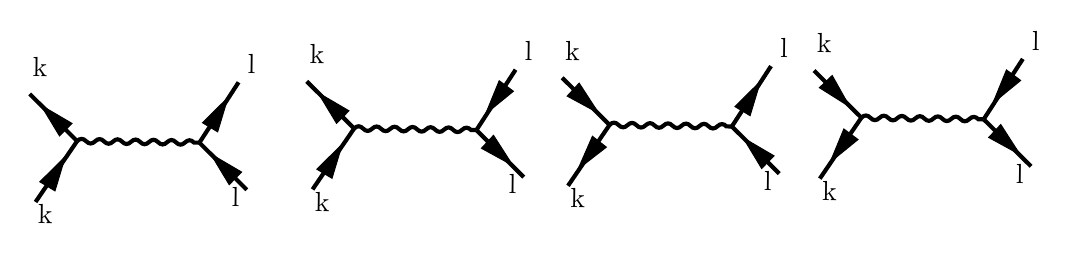
\begin{tikzpicture}[x=0.65pt,y=0.65pt,yscale=-1,xscale=1]
%uncomment if require: \path (0,705); %set diagram left start at 0, and has height of 705

%Straight Lines [id:da613823184290475] 
\draw [line width=1.5]    (69.46,540.64) .. controls (71.15,538.99) and (72.81,539.01) .. (74.46,540.7) .. controls (76.11,542.39) and (77.77,542.41) .. (79.46,540.77) .. controls (81.15,539.12) and (82.81,539.14) .. (84.46,540.83) .. controls (86.11,542.52) and (87.77,542.54) .. (89.46,540.9) .. controls (91.15,539.25) and (92.81,539.27) .. (94.46,540.96) .. controls (96.11,542.65) and (97.77,542.67) .. (99.46,541.03) .. controls (101.15,539.38) and (102.81,539.4) .. (104.46,541.09) .. controls (106.11,542.78) and (107.77,542.8) .. (109.46,541.15) .. controls (111.15,539.51) and (112.81,539.53) .. (114.46,541.22) .. controls (116.11,542.91) and (117.77,542.93) .. (119.46,541.28) .. controls (121.15,539.64) and (122.81,539.66) .. (124.45,541.35) .. controls (126.1,543.04) and (127.76,543.06) .. (129.45,541.41) .. controls (131.14,539.77) and (132.8,539.79) .. (134.45,541.48) -- (137.45,541.52) -- (137.45,541.52) ;
%Straight Lines [id:da6353755682299548] 
\draw [line width=1.5]    (43.13,514.46) -- (69.46,540.64) ;
%Straight Lines [id:da6254606220772768] 
\draw [line width=1.5]    (137.45,541.52) -- (163.78,567.69) ;
%Straight Lines [id:da5480869883300985] 
\draw [line width=1.5]    (69.46,540.64) -- (46.35,574.51) ;
%Straight Lines [id:da49445752084181116] 
\draw [line width=1.5]    (159.22,507.96) -- (137.45,541.52) ;
%Shape: Triangle [id:dp022384072825595847] 
\draw  [fill={rgb, 255:red, 0; green, 0; blue, 0 }  ,fill opacity=1 ] (49.47,520.82) -- (66.54,530.81) -- (59.69,537.75) -- cycle ;
%Shape: Triangle [id:dp5669679661948073] 
\draw  [fill={rgb, 255:red, 0; green, 0; blue, 0 }  ,fill opacity=1 ] (143.8,547.87) -- (160.86,557.87) -- (154.01,564.81) -- cycle ;
%Shape: Triangle [id:dp23872151900315752] 
\draw  [fill={rgb, 255:red, 0; green, 0; blue, 0 }  ,fill opacity=1 ] (153.28,516.53) -- (147.58,535.46) -- (139.22,530.44) -- cycle ;
%Shape: Triangle [id:dp5504301680867448] 
\draw  [fill={rgb, 255:red, 0; green, 0; blue, 0 }  ,fill opacity=1 ] (62.85,549.36) -- (57.15,568.3) -- (48.79,563.27) -- cycle ;
%Straight Lines [id:da6839577763606166] 
\draw [line width=1.5]    (223.46,533.64) .. controls (225.15,531.99) and (226.81,532.01) .. (228.46,533.7) .. controls (230.11,535.39) and (231.77,535.41) .. (233.46,533.77) .. controls (235.15,532.12) and (236.81,532.14) .. (238.46,533.83) .. controls (240.11,535.52) and (241.77,535.54) .. (243.46,533.9) .. controls (245.15,532.25) and (246.81,532.27) .. (248.46,533.96) .. controls (250.11,535.65) and (251.77,535.67) .. (253.46,534.03) .. controls (255.15,532.38) and (256.81,532.4) .. (258.46,534.09) .. controls (260.11,535.78) and (261.77,535.8) .. (263.46,534.15) .. controls (265.15,532.51) and (266.81,532.53) .. (268.46,534.22) .. controls (270.11,535.91) and (271.77,535.93) .. (273.46,534.28) .. controls (275.15,532.64) and (276.81,532.66) .. (278.45,534.35) .. controls (280.1,536.04) and (281.76,536.06) .. (283.45,534.41) .. controls (285.14,532.77) and (286.8,532.79) .. (288.45,534.48) -- (291.45,534.52) -- (291.45,534.52) ;
%Straight Lines [id:da9240174823017793] 
\draw [line width=1.5]    (197.13,507.46) -- (223.46,533.64) ;
%Straight Lines [id:da42566261374485415] 
\draw [line width=1.5]    (291.45,534.52) -- (317.78,560.69) ;
%Straight Lines [id:da016054446409110024] 
\draw [line width=1.5]    (223.46,533.64) -- (200.35,567.51) ;
%Straight Lines [id:da7774023230842375] 
\draw [line width=1.5]    (313.22,500.96) -- (291.45,534.52) ;
%Shape: Triangle [id:dp3043226594104913] 
\draw  [fill={rgb, 255:red, 0; green, 0; blue, 0 }  ,fill opacity=1 ] (203.47,513.82) -- (220.54,523.81) -- (213.69,530.75) -- cycle ;
%Shape: Triangle [id:dp9365361434860027] 
\draw  [fill={rgb, 255:red, 0; green, 0; blue, 0 }  ,fill opacity=1 ] (311.63,554.14) -- (294.29,544.63) -- (300.94,537.5) -- cycle ;
%Shape: Triangle [id:dp13172855405910544] 
\draw  [fill={rgb, 255:red, 0; green, 0; blue, 0 }  ,fill opacity=1 ] (296.64,525.44) -- (304.12,507.14) -- (311.96,512.94) -- cycle ;
%Shape: Triangle [id:dp6150273572328407] 
\draw  [fill={rgb, 255:red, 0; green, 0; blue, 0 }  ,fill opacity=1 ] (216.85,542.36) -- (211.15,561.3) -- (202.79,556.27) -- cycle ;
%Straight Lines [id:da10558670890674016] 
\draw [line width=1.5]    (505.46,527.64) .. controls (507.15,525.99) and (508.81,526.01) .. (510.46,527.7) .. controls (512.11,529.39) and (513.77,529.41) .. (515.46,527.77) .. controls (517.15,526.12) and (518.81,526.14) .. (520.46,527.83) .. controls (522.11,529.52) and (523.77,529.54) .. (525.46,527.9) .. controls (527.15,526.25) and (528.81,526.27) .. (530.46,527.96) .. controls (532.11,529.65) and (533.77,529.67) .. (535.46,528.03) .. controls (537.15,526.38) and (538.81,526.4) .. (540.46,528.09) .. controls (542.11,529.78) and (543.77,529.8) .. (545.46,528.15) .. controls (547.15,526.51) and (548.81,526.53) .. (550.46,528.22) .. controls (552.11,529.91) and (553.77,529.93) .. (555.46,528.28) .. controls (557.15,526.64) and (558.81,526.66) .. (560.45,528.35) .. controls (562.1,530.04) and (563.76,530.06) .. (565.45,528.41) .. controls (567.14,526.77) and (568.8,526.79) .. (570.45,528.48) -- (573.45,528.52) -- (573.45,528.52) ;
%Straight Lines [id:da4301121902778472] 
\draw [line width=1.5]    (479.13,501.46) -- (505.46,527.64) ;
%Straight Lines [id:da8070089193956563] 
\draw [line width=1.5]    (573.45,528.52) -- (599.78,554.69) ;
%Straight Lines [id:da9369302080120971] 
\draw [line width=1.5]    (505.46,527.64) -- (482.35,561.51) ;
%Straight Lines [id:da6514758529059829] 
\draw [line width=1.5]    (595.22,494.96) -- (573.45,528.52) ;
%Shape: Triangle [id:dp46358512529050333] 
\draw  [fill={rgb, 255:red, 0; green, 0; blue, 0 }  ,fill opacity=1 ] (498.9,521.5) -- (482.16,510.96) -- (489.23,504.24) -- cycle ;
%Shape: Triangle [id:dp38044017958960863] 
\draw  [fill={rgb, 255:red, 0; green, 0; blue, 0 }  ,fill opacity=1 ] (593.63,548.14) -- (576.29,538.63) -- (582.94,531.5) -- cycle ;
%Shape: Triangle [id:dp28303426408257704] 
\draw  [fill={rgb, 255:red, 0; green, 0; blue, 0 }  ,fill opacity=1 ] (578.64,519.44) -- (586.12,501.14) -- (593.96,506.94) -- cycle ;
%Shape: Triangle [id:dp44406046766962526] 
\draw  [fill={rgb, 255:red, 0; green, 0; blue, 0 }  ,fill opacity=1 ] (488.19,552.26) -- (495.71,533.97) -- (503.54,539.79) -- cycle ;
%Straight Lines [id:da7271479706009089] 
\draw [line width=1.5]    (365.46,531.64) .. controls (367.15,529.99) and (368.81,530.01) .. (370.46,531.7) .. controls (372.11,533.39) and (373.77,533.41) .. (375.46,531.77) .. controls (377.15,530.12) and (378.81,530.14) .. (380.46,531.83) .. controls (382.11,533.52) and (383.77,533.54) .. (385.46,531.9) .. controls (387.15,530.25) and (388.81,530.27) .. (390.46,531.96) .. controls (392.11,533.65) and (393.77,533.67) .. (395.46,532.03) .. controls (397.15,530.38) and (398.81,530.4) .. (400.46,532.09) .. controls (402.11,533.78) and (403.77,533.8) .. (405.46,532.15) .. controls (407.15,530.51) and (408.81,530.53) .. (410.46,532.22) .. controls (412.11,533.91) and (413.77,533.93) .. (415.46,532.28) .. controls (417.15,530.64) and (418.81,530.66) .. (420.45,532.35) .. controls (422.1,534.04) and (423.76,534.06) .. (425.45,532.41) .. controls (427.14,530.77) and (428.8,530.79) .. (430.45,532.48) -- (433.45,532.52) -- (433.45,532.52) ;
%Straight Lines [id:da7854992580693345] 
\draw [line width=1.5]    (339.13,505.46) -- (365.46,531.64) ;
%Straight Lines [id:da338940395062972] 
\draw [line width=1.5]    (433.45,532.52) -- (459.78,558.69) ;
%Straight Lines [id:da20114032104584845] 
\draw [line width=1.5]    (365.46,531.64) -- (342.35,565.51) ;
%Straight Lines [id:da47776944835115154] 
\draw [line width=1.5]    (455.22,498.96) -- (433.45,532.52) ;
%Shape: Triangle [id:dp9747602816540912] 
\draw  [fill={rgb, 255:red, 0; green, 0; blue, 0 }  ,fill opacity=1 ] (359.33,525.05) -- (341.95,515.63) -- (348.56,508.47) -- cycle ;
%Shape: Triangle [id:dp8973952534123313] 
\draw  [fill={rgb, 255:red, 0; green, 0; blue, 0 }  ,fill opacity=1 ] (439.8,538.87) -- (456.86,548.87) -- (450.01,555.81) -- cycle ;
%Shape: Triangle [id:dp7615505790794537] 
\draw  [fill={rgb, 255:red, 0; green, 0; blue, 0 }  ,fill opacity=1 ] (449.28,507.53) -- (443.58,526.46) -- (435.22,521.44) -- cycle ;
%Shape: Triangle [id:dp860067401387033] 
\draw  [fill={rgb, 255:red, 0; green, 0; blue, 0 }  ,fill opacity=1 ] (348.02,556.14) -- (355.95,538.02) -- (363.64,544.01) -- cycle ;

% Text Node
\draw (46.35,574.51) node [anchor=north west][inner sep=0.75pt]  [rotate=-0.74] [align=left] {k};
% Text Node
\draw (43.41,492.46) node [anchor=north west][inner sep=0.75pt]  [rotate=-0.74] [align=left] {k};
% Text Node
\draw (154.01,564.81) node [anchor=north west][inner sep=0.75pt]  [rotate=-0.74] [align=left] {l};
% Text Node
\draw (162.97,490.91) node [anchor=north west][inner sep=0.75pt]  [rotate=-0.74] [align=left] {l};
% Text Node
\draw (200.35,567.51) node [anchor=north west][inner sep=0.75pt]  [rotate=-0.74] [align=left] {k};
% Text Node
\draw (197.41,485.46) node [anchor=north west][inner sep=0.75pt]  [rotate=-0.74] [align=left] {k};
% Text Node
\draw (308.01,557.81) node [anchor=north west][inner sep=0.75pt]  [rotate=-0.74] [align=left] {l};
% Text Node
\draw (316.97,483.91) node [anchor=north west][inner sep=0.75pt]  [rotate=-0.74] [align=left] {l};
% Text Node
\draw (482.35,561.51) node [anchor=north west][inner sep=0.75pt]  [rotate=-0.74] [align=left] {k};
% Text Node
\draw (479.41,479.46) node [anchor=north west][inner sep=0.75pt]  [rotate=-0.74] [align=left] {k};
% Text Node
\draw (590.01,551.81) node [anchor=north west][inner sep=0.75pt]  [rotate=-0.74] [align=left] {l};
% Text Node
\draw (598.97,477.91) node [anchor=north west][inner sep=0.75pt]  [rotate=-0.74] [align=left] {l};
% Text Node
\draw (342.35,565.51) node [anchor=north west][inner sep=0.75pt]  [rotate=-0.74] [align=left] {k};
% Text Node
\draw (339.41,483.46) node [anchor=north west][inner sep=0.75pt]  [rotate=-0.74] [align=left] {k};
% Text Node
\draw (450.01,555.81) node [anchor=north west][inner sep=0.75pt]  [rotate=-0.74] [align=left] {l};
% Text Node
\draw (458.97,481.91) node [anchor=north west][inner sep=0.75pt]  [rotate=-0.74] [align=left] {l};


\end{tikzpicture}
\end{equation}
Hence the only graphs occurring in the series for the ground state energy are 
\begin{equation}
    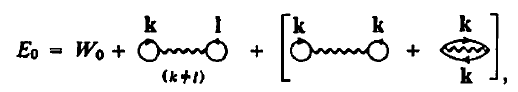
\includegraphics[width=0.8\textwidth]{screenshots/pure-hartree-diam.PNG}
    \label{pure-hartree-diam}
\end{equation}
Note that \textbf{the propagator lines in these diagrams are all hole lines. Also the diagrams in brackets violate the exclusion principle since there are simultaneously two hole lines in state $\mathbf{k}$}.
\begin{equation}E_{0}=\sum_{k<k=7} \epsilon_{k}+\frac{1}{2} \sum_{\substack{k, l<k_F\\\mathbf{k}\neq\mathbf{l}}}^{\prime} V_{k l k l}
\label{pure-hartree-E0}
\end{equation}
The $\mathbf{k=l}$ graphs cancel because of the fermion loop in bubble diagram.

Now let us get the quasi particle energies, $\epsilon_k^{\prime}$, from the poles of the Green's function. In this case, the propagator is given exactly by the sum over just the bubble graphs:
\begin{equation}
    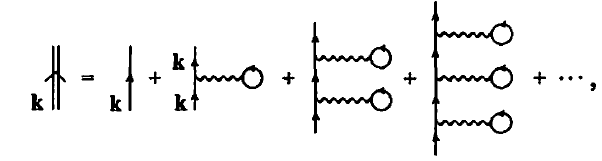
\includegraphics[width=0.8\textwidth]{screenshots/pure-hartree-diam-series.PNG}
    \label{pure-hartree-diam-series}
\end{equation}
Series (\ref{pure-hartree-diam-series}) was summed and gives the result for quasi particle energy, as shown in chapter 4,
\begin{equation}\begin{array}{l}
\epsilon_{k}^{\prime}=\epsilon_{k}+\sum_{l<k_F} V_{k l k l}, \quad k>k_{F} \\
\tau_{k}=\infty
\end{array}
\label{pure-hartree-E-particle}
\end{equation}
In the case of quasi holes we just sum
\begin{equation}
    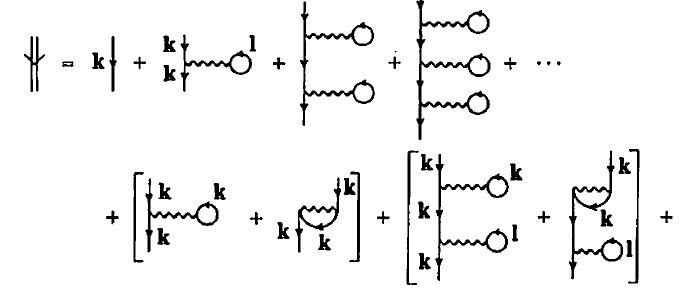
\includegraphics[width=0.8\textwidth]{screenshots/pure-hartree-hole-diam-series.PNG}
    \label{pure-hartree-hole-diam-series}
\end{equation}
The bracketed diagrams cancel because of the fermion loop and we get the result:
\begin{equation}\begin{aligned}
&\epsilon_{k}^{\prime}=\epsilon_{k}+\sum_{l<k_{F}}{}^{\prime} V_{k l k l}, \quad k<k_{F}\\
&\tau_{k}=\infty
\end{aligned}
\label{pure-hartree-E-hole}
\end{equation}

Finally, we need the interaction between quasi particles ($f$-term in (\ref{pure-hartree-hamil})).This can be obtained from the various two-particle propagators. Consider the particle-particle propagator first. In the present case, this is given by the sum:
\begin{equation}
    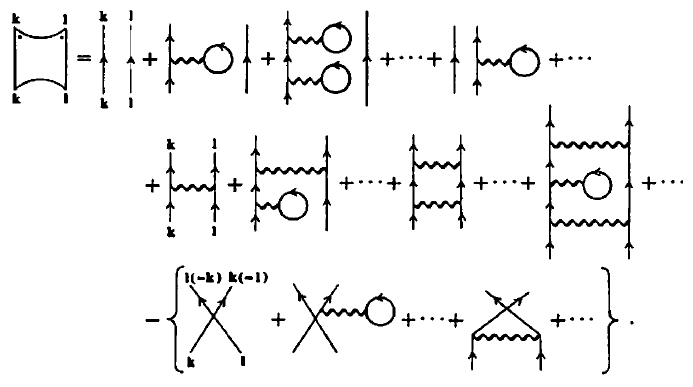
\includegraphics[width=0.8\textwidth]{screenshots/particle-particle-diam-series.PNG}
    \label{particle-particle-diam-series}
\end{equation}
The crossed "exchange" diagrams in the brackets in (\ref{particle-particle-diam-series}) contribute only when $\mathbf{k}=\mathbf{l}$. because the labels on the incoming and outgoing lines in each diagram must match those of $G_2$ on the left. \redp{\textbf{Since these diagrams are negative, they cancel all the uncrossed diagrams when $\mathbf{k=l}$, so $G_2=0$ for $\mathbf{k=l}$}}.

We can greatly simplify (\ref{particle-particle-diam-series}) in the following way:
Consider the diagram subset consisting of more and more bubbles inserted into the first propagator,i.e.,:
\begin{equation}
    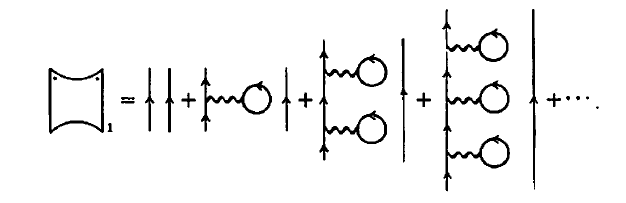
\includegraphics[width=0.8\textwidth]{screenshots/particle-particle-diam-series-2.PNG}
    \label{particle-particle-diam-series-2}
\end{equation}
This can be summed as:
\begin{equation}
    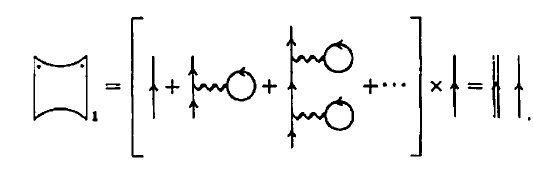
\includegraphics[width=0.8\textwidth]{screenshots/particle-particle-diam-series-3.PNG}
\end{equation}
Similarly, we sum over all bubble insertions in all bare propagators, leading to a sum in which all propagators are clothed,\redp{i.e.,} in which all propagators are the quasi particle propagators:
\begin{equation}
    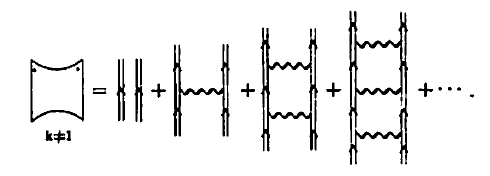
\includegraphics[width=0.8\textwidth]{screenshots/particle-particle-diam-series-4.PNG}
\end{equation}
In this form, we can see that the quasi particle interaction is:$V=V_{klkl}(l\neq k), V=0(l=k)$. Similar arguments applied to the particle-hole and hole-hole propagators yield this same interaction.

We can now combine these results into a Hamiltonian of form (\ref{pure-hartree-hamil}). The expressions for $E_0$ and $\epsilon_q^{\prime}$ are in (\ref{pure-hartree-E0}),(\ref{pure-hartree-E-particle}), and (\ref{pure-hartree-E-hole}). The interaction term $f$ in (\ref{pure-hartree-hamil}) will have the form
$$H_{1}=\frac{1}{2} \sum_{k, l, m, n} V_{k l m n} c^{\dagger}, c_{k}^{\dagger} c_{m} c_{n}$$
since the quasi particles here are fermions.

Letting $A_{k}^{\dagger}, A_{k}, B_{k}^{\dagger}, B_{k},$ be the quasi particle and quasi hole operators we find
\begin{equation}\begin{aligned}
H^{\prime}=[&\sum_{k<k_{F}} \epsilon_{k}+\frac{1}{2} \sum_{k,l<k_F}^{\prime} V_{k l k l}]+\\
&+\sum_{k<k_{F}}\left(\epsilon_{k}+\sum_{l<k_{p}} V_{k l k l}\right) A_{k}^{\dagger} A_{k}-\sum_{k<k_{F}}\left(\epsilon_{k}+\sum_{l<k_{F}}^{\prime} V_{klkl}\right) B_{k}^{\dagger} B_{k}+\\
&+\frac{1}{2} \sum_{l,k>k_{F}}^{\prime} V_{kl k l} A_{l}^{\dagger} A_{k}^{\dagger} A_{k} A_{l}-\sum_{\substack{k>k_{F}\\l<k_F}} V_{k l k l} B_{l}^{\dagger} A_{k}^{\dagger} A_{k} B_{l}+\\
&+\frac{1}{2} \sum_{\substack{k<k_F\\l<k_F}}^{\prime} V_{klkl} B_{l}^{\dagger} B_{k}^{\dagger} B_{k} B_{l}
\end{aligned}\end{equation}
Observe that in the particle-particle and hole-hole interaction terms, \textbf{it is necessary to put in a factor $\frac{1}{2}$ to avoid counting interactions twice when we sum freely over $\mathbf{k}$ and $\mathbf{l}$.} Note that the $(-)$ sign in the $B_{k}^{1} B_{k}$ term is put in because the hole energies (and therefore the quasi hole energies) are negative. The (-) in the $B_{l}^{t} A_{k}^{1} A_{k} B_{l}$ term occurs for the following reason: \bluep{The energy of a quasi particle in, say, state $k_1>k_F$, includes interactions with all particles in the filled Fermi sea. But if there is a hole in, say, state $l_1<k_F$, then the corresponding energy,$V_{k_1l_1k_1l_1}$ does not exist, and should be subtracted from the quasi particle energy. The term $-V_{k_1l_1k_1l_1}B_{l_1}^{\dagger}A_{k_1}^{\dagger}A_{k_1}B_{l_1}$  takes care of this substraction.}

\subsection{Crude calculation of quasi particle lifetime}
We mentioned that \redp{the quasi particle picture breaks down if the energy is two far away from the Fermi energy.} In a Fermi system, since one deals with particle-like excitation above $\epsilon_F^{\prime}$ (the Fermi energy of the interacting system), and hole-like ones below, the criterion is taken relative to the Fermi energy, i.e.:
\begin{equation}\frac{1}{\tau_{k}} \ll \epsilon_{k}^{\prime}-\epsilon_{F}^{\prime}\end{equation}
In the pure Hartree model,$\tau_k=\infty$, so this is satisfied for any $k$. But this is not true in general. In fact, we are now going to show that in most Fermi systems the quasi particle lifetime obeys
\begin{equation}\frac{1}{\tau_{k}} \propto\left(\epsilon_{k}^{\prime}-\epsilon_{F}^{\prime}\right)^{2}
\label{lifetime-criterion}
\end{equation}
Here we will give a crude quasi-proof of (\ref{lifetime-criterion}).

\bluep{The lifetime of a quasi particle in momentum state $\mathbf{k}$ will be the \textbf{inverse of the transition probability per second that the quasi particle will be scattered out of state $\mathbf{k}$ by collisions with other quasi particles}.} Let us pretend that quasi particle collisions are like those between real particles (they are not, actually, since quasi particles can have a 'retarded', i.e., time-dependent, interaction even when the bare particles interact instantaneously) and calculate the transition probability out of state $\mathbf{k}_1$ for a particle in state $\mathbf{k}_1$, where $|\mathbf{k}_1|\geq k_F$. In a typical interaction, the particle will collide with a particle in state $|\mathbf{k}_2|\leq k_F$ and final state will be a particle in $\mathbf{k}_3$ and $\mathbf{k}_4$, where
\begin{equation}\mathbf{k}_{4}=\mathbf{k}_{1}+\mathbf{k}_{2}-\mathbf{k}_{3}\end{equation}
The transition probability is
\begin{equation}W_{k_{1}} \propto \int d^{3} k_{2} \int d^{3} k_{3}\left|V_{k_{3}, k_{1}+k_{2}-k_{3}, k_{1}, k_{2}}\right|^{2}
\label{crude-quasi-interaction-probability}
\end{equation}
To evaluate (\ref{crude-quasi-interaction-probability}) we note that by the Pauli principle all states under $k_F$ are occupied so that \begin{equation}\left|\mathbf{k}_{3}\right| \geqslant k_{F}, \quad\left|\mathbf{k}_{4}\right| \geqslant k_{F}
\label{crude-proof-1}
\end{equation}
by conservation of energy,
\begin{equation}k_{1}^{2}+k_{2}^{2}=k_{3}^{2}+k_{4}^{2}
\label{crude-proof-2}
\end{equation}
The equations above imply that 
\begin{equation}k_{1}^{2}+k_{2}^{2} \geqslant 2 k_{F}^{2}
\label{crude-proof-3}
\end{equation}
Consider first the limiting case when $\left|\mathbf{k}_{1}\right|=k_{F} .$ Then by (\ref{crude-proof-3})$, k_{2}^{2} \geqslant k_{F}^{2} .$ But since $\left|\mathbf{k}_{2}\right| \leqslant k_{F},$ this implies $\left|\mathbf{k}_{2}\right|=k_{F}$. Similarly, $\left|\mathbf{k}_{3}\right|=\left|\mathbf{k}_{4}\right|=k_{F} .$ \textbf{That is, all momenta lie on the Fermi sphere.} Suppose now that $\left|\mathbf{k}_{1}\right|=k_{F}+\delta$ where $k_{F} \gg \delta>0 .$ Then by (\ref{crude-proof-3}) $,\left|\mathbf{k}_{2}\right| \geqslant k_{F}-\delta .$ Similarly, since $\left|\mathbf{k}_{2}\right| \leqslant k_{F},$ we have that in order to satisfy (\ref{crude-proof-2}), $\left|\mathbf{k}_{\mathbf{3}}\right|,\left|\mathbf{k}_{4}\right|$ must be less than $k_{F}+\delta .$ Hence all momenta lie in a shell of thickness $\delta=\left|\mathbf{k}_{1}\right|-k_{F}$ around the Fermi sphere. Assuming there's nothing peculiar about the behaviour of $V$, the integral over the $\mathbf{k}_{2}$ -shell gives a factor $\propto 4 \pi k_{F}^{2}\left(\left|\mathbf{k}_{1}\right|-k_{F}\right),$ and the same for the $\mathbf{k}_{3}$ -shell, so
\begin{equation}W_{k_{1}} \propto\left(\left|\mathbf{k}_{1}\right|-k_{F}\right)^{2}\end{equation}
But
\begin{equation}\begin{aligned}
\epsilon_{k_{1}}-\epsilon_{p} \propto\left(k_{1}^{2}-k_{F}^{2}\right) &=\left(\left|\mathbf{k}_{1}\right|-k_{P}\right)\left(\left|\mathbf{k}_{1}\right|+k_{F}\right) \\
& \approx 2 k_{F}\left(\left|\mathbf{k}_{1}\right|-k_{F}\right)
\end{aligned}\end{equation}
Whence
\begin{equation}\frac{1}{\tau_{k}}=W_{k} \propto\left(\epsilon_{k}-\epsilon_{F}\right)^{2}\end{equation}

\subsection{General form of quasi particle propagator}
We have learned that the single-particle propagator or "Green's function" is defined as
\begin{equation}G\left(k_{2}, k_{1}, t_{2}-t_{1}\right)=G^{+}\left(k_{2}, k_{1}, t_{2}-t_{1}\right)_{t_{2}>t_{1}}+G^{-}\left(k_{2}, k_{1}, t_{2}-t_{1}\right)_{t_{2}\leq t_{1}}\end{equation}
where $iG^+(k_2,k_1,t_2-t1)$ is probability amplitude that if at time $t_{1}$ we add a particle in $\phi_{k_{1}}$ to the interacting system in its ground state, then at time $t_{2}$ the system will be in its ground state with an added particle in $\phi_{k_{2}}$, and $-iG^-(k_2,k_1,t_2-t1)$ is probability amplitude that if at time $t_{2}$ we add a hole in $\phi_{z_{2}}$ to the interacting system in its ground state, then at time $t_{1}$ the system will be in its ground state with an added hole in $\phi_{k_{1}}$. (\redp{\textbf{The "-" sign on $G^-$ is for fermions; bosons have a $+iG^-$ instead}}.) These results may be written in a compact way by introducing the functions
\begin{equation}\theta_{x}\left\{\begin{array}{lll}
=1, & \text { for } x>1 \\
=0, & \text { for } x<1
\end{array} ; \quad \delta_{k}\left\{\begin{array}{lll}
&=+\delta, \quad \epsilon_{k}>\epsilon_{F} \\
&=-\delta, \quad \epsilon_{k}<\epsilon_{F}
\end{array}\right.\right.\end{equation}
Letting $t=t_2-t_1$, this c=gives
\begin{equation}\begin{aligned}
G_{0}(k, t) &=-i\left[\theta_{t} \theta_{\epsilon_k-\epsilon_F }e^{-i\epsilon_{k} t}-\theta_{-t} \theta_{\epsilon_F-\epsilon_{k}} e^{-i\epsilon_kt}\right], \quad t \neq 0 \\
&=+i \theta_{t_{p-t_{2}}}, \quad t=0
\end{aligned}
\label{combined-G0-in-k-t-space}
\end{equation}
and
\begin{equation}G_{0}(k, \omega)=\frac{1}{\omega-\epsilon_{k}+i \delta_{k}}\end{equation}

Now in Chapter 3 we argue that in systems describable by quasi particles, $G$ will look like $G_{0}$ except for replacing $\epsilon_{\mathbf{k}}$ by $\epsilon_{\mathbf{k}}^{\prime}$, introducing a lifetime $\tau_{k},$ and an amplitude factor, $Z_{k}$ as in (\ref{partial-occ-factor-t},\ref{partial-occ-factor-k}). However, this is not quite right, because it neglects the fact that when the bare particle is first put into the system, it will take some finite time, say $t_{c},$ for it to become 'clothed' so it will not act like a quasi particle until $t_{2}-t_{1}>t_{c} .$ Further, it can be shown that the quasi particle expression for the propagator is no longer valid when $t_{2}-t_{1} \gg \tau_{k}$ where $\tau_{k}$ is the lifetime. For this reason \textbf{it is necessary to write the propagator as the sum of a pure quasi particle part plus a correction term which will be important for $t<t_{e}$ and $t>\tau_{k}$}. This consideration yields (setting $t=t_2-t_1$ and $t\neq0$):
\begin{equation}\begin{aligned}
G_{\substack{quasi\\particle}}(k, t)=&-i Z_{k}\left[\theta_{t} \theta_{\epsilon^{\prime}_{k}-\epsilon^{\prime}_F} e^{-i\left(\epsilon_{k}^{\prime}-i \tau_{k}^{-1}\right) t}-\right.\\
&\left.-\theta_{-t} \theta_{\epsilon^{\prime}_F-\epsilon_{k}^{\prime}} e^{-i\left(\epsilon_{k}^{\prime}+i_{\tau_{k}}^{-1}\right)t}\right]+F(k, t)
\end{aligned}\end{equation}
where $0<Z_{k} \leqslant 1\left(Z_{k} \text { independent of } t\right)$. \bluep{Don't be scared by the term of $\epsilon_k^{\prime}\pm i\tau_k^{-1}$. For $G_0$ we have $\epsilon_k\pm i\delta$. Since $\delta$ is infinitesimally small, so we have instead $\epsilon_k$ in the exponential of $G_0$. So they are the same thing with different lifetime.(finite vs. infinite)}

Taking the Fourier transform :
\begin{equation}G_{\substack{quasi\\particle}}(k, \omega)=\frac{Z_{k}}{\omega-\epsilon_{k}^{\prime}+i\left[2 \theta_{\epsilon^{\prime}_{k}-\epsilon_F^{\prime}}-1\right] \tau_{k}^{-1}}+F(k, \omega)\end{equation}
\redp{\textbf{It must be remembered that these are bona fide quasi particles only if }}
\begin{equation}\frac{1}{\tau_{k}} \ll \epsilon_{k}^{\prime}-\epsilon_{F}^{\prime}\end{equation}
\newpage
\section{The Single-Particle Propagator Re-Visited}
\subsection{Mathematical expression for the single-particle Green's function propagator}
The closed mathematical expression for the propagator,$G$, appears usually in one of two forms:
\begin{equation}\begin{aligned}
G\left(k_{2}, k_{1}, t_{2}-t_{1}\right) &=-i\left\langle\Psi_{0}\left|T\left\{c_{k_{2}}\left(t_{2}\right) c^{\dagger}_{k_{1}}\left(t_{1}\right)\right\}\right| \Psi_{0}\right\rangle \\
G\left(\mathrm{r}_{2}, \mathrm{r}_{1}, t_{2}-t_{1}\right) &=-i\left\langle\Psi_{0}\left|T\left\{\psi\left(\mathrm{r}_{2}, t_{2}\right) \psi^{\dagger}\left(\mathrm{r}_{1}, t_{1}\right)\right\}\right| \Psi_{0}\right\rangle
\end{aligned}
\label{sandwitch-defi-G}
\end{equation}
We shall only consider the first form-the second may be analysed in a similar way. First, $\Psi_{0}$ is the exact normalized wave function of the ground state of the interacting $N$ -particle system. The operators $c_{k}(t), c_{k}^{\dagger}(t)$ respectively, destroy and create a particle in state $k$ at time $t .$ More precisely, they are the ordinary $c_{k}, c_{k}^{\dagger}$ transformed to \redp{'Heisenberg picture'}, defined by
\begin{equation}\begin{array}{l}
c^{\dagger}_{k_{1}}\left(t_{1}\right)=e^{+i Ht_{1}} c_{k_{1}} e^{-i H t_{1}} \\
c_{k_{2}}\left(t_{2}\right)=e^{+i Ht_2} c_{k_{2}} e^{-i Ht_{2}}
\end{array}\end{equation}
Finally the Wick time-ordering operator, T, is defined by
\begin{imp}
\begin{equation}
\begin{aligned}
T\left\{A\left(t_{1}\right) B\left(t_{2}\right) \ldots\right\}=&(-1)^{P} \times\begin{varwidth}[t]{\linewidth}operators rearranged so that time\\decreases from left to right, assuming\\no two times are equal,\end{varwidth}\\
&=(-1)^P\times\begin{varwidth}[t]{\linewidth}operators rearranged so all $c^{\dagger}$ 's (or\\ $a^{\dagger}$' s or $b$'s) stand to the left of $c$'s $($ or\\ $a$'s or $\boldsymbol{b}^{\dagger}$ 's ) for the case of equal\\ times)\end{varwidth}
\end{aligned}
\end{equation}
where $P$ is the number of interchanges of operators required to get the operators in the proper time order, starting with the order given in the brackets.
\end{imp}
Thus, 
\begin{equation}\begin{aligned}
T\left\{c_{k_{2}}\left(t_{2}\right) c_{k_{1}}\left(t_{1}\right)\right\} &=c_{k_{2}}\left(t_{2}\right) c^{\dagger}_{k_{1}}\left(t_{1}\right) \text { for } t_{2}>t_{1} \\
&=-c_{k_{1}}^{\dagger}\left(t_{1}\right) c_{k_{2}}\left(t_{2}\right) \text { for } t_{2} \leqslant t_{1}
\end{aligned}\end{equation}
and
\begin{equation}\begin{aligned}
G &=G^{+}\left(k_{2}, k_{1}, t_{2}-t_{1}\right)=-i\left\langle\Psi_{0}\left|c_{k_{2}}\left(t_{2}\right) c^{\dagger}_{k_{1}}\left(t_{1}\right)\right| \Psi_{0}\right\rangle, \quad t_{2}>t_{1} \\
&=G^{-}\left(k_{2}, k_{1}, t_{2}-t_{1}\right)=+i\left\langle\Psi_{0}\left|c^{\dagger}_{k_{1}}\left(t_{1}\right) c_{k_{2}}\left(t_{2}\right)\right| \Psi_{0}\right\rangle, \quad t_{2} \leqslant t_{1}
\end{aligned}\end{equation}
Consider the $t_2>t_1$ case first, we have
\begin{equation}G^{+}=-\underbrace{I\left\langle\Psi_{0}\right| e^{i Ht_{2}} c_{k_{2}}}_{B^{\dagger}} \underbrace{e^{-i H\left(t_{2}-t_{1}\right)} c^{\dagger}_{k_{1}} e^{-i Ht_{1}}\left|\Psi_{0}\right\rangle}_{A}
\label{G+=BA}
\end{equation}
Now \redp{$exp(-iHt)$ is the time development operator}, so that $exp(-iHt_1)|\Psi_0\rangle$ is the ground state at time $t_1$, and $c^{\dagger}_{k_1}exp(-iHt_1)|\Psi_0\rangle$ is the state with one particle in $\phi_{k_1}$ added to the ground state at time $t_1$. Hence $\mathbf{A}$ is the state of the system at time $t_2$ when a particle $\phi_{k_1}$ was added at $t_1$. The $B^{\dagger}$ is
\begin{equation}B^{\dagger}=\overline{c^{\dagger}_{k_{2}} e^{-iH t_{2}} |\Psi_{0}}\rangle\end{equation}
This is \bluep{the complex conjugate of the state with one particle in $\phi_{k_2}$ added to the ground state at time $t_2$.} Hence we obtain
\begin{equation}
    \begin{aligned}
    G^+=B^{\dagger}A&=\text{component of B along A}\\
    &=\begin{varwidth}[t]{\linewidth}
    probability amplitude that the state of the system\\
    at $t_{2},$ when a particle in $\phi_{k_{1}}$ was added to the\\ 
    ground state at $t_{1},$ is the state with one particle in \\
    $\phi_{k_{2}}$ added to the ground state at time $t_{2}$
    \end{varwidth}
    \end{aligned}
\end{equation}
It is a good brain-building exercise to show how (\ref{sandwitch-defi-G}) boils down to the expression for the free propagator (\ref{combined-G0-in-k-t-space}), in the non-interacting case. The non-interacting Hamiltonian and ground state are given by
\begin{equation}H_{0}=\sum_{p} \epsilon_{p} c_{p}^{\dagger} c_{p}, \quad H_{0}\left|\Phi_{0}\right\rangle=\sum_{p<k_{F}} \epsilon_{p}\left|\Phi_{0}\right\rangle, \quad\left|\Phi_{0}\right\rangle=\left|111 \ldots 1_{F} 000 \ldots\right\rangle\end{equation}
Let us calculate just $G_0^+$ setting $t_1=0,t_2=t$:
\begin{equation}G_{0}^{+}(k, t)=-i\left\langle\Phi_{0}\left|e^{+i H_{0}t} c_{k} e^{-iH_{0}t} c_{k}^{\dagger}\right| \Phi_{0}\right\rangle \theta_{t}\end{equation}
In an obvious notation,
\begin{equation}c_{k}^{\dagger}\left|\Phi_{0}\right\rangle=(-1)^{N}\left|\Phi_{0}, 1_{k}\right\rangle \theta_{\epsilon_k-\epsilon_F}\end{equation}
Thus $k$ must be greater than $k_F$. Now
\begin{equation}H_{0}\left|\Phi_{0}, 1_{k}\right\rangle=\sum_{p} \epsilon_{p} c_{p}^{\dagger} c_{p}\left|\Phi_{0}, 1_{k}\right\rangle=\left[\sum_{p<k_{F}} \epsilon_{p}+\epsilon_{k}\right]\left|\Phi_{0} 1_{k}\right\rangle\end{equation}
Thus
\begin{equation}c_{k} e^{-i H_{0} t}\left|\Phi_{0}, 1_{k}\right\rangle=(-1)^{N}\left|\Phi_{0}\right\rangle \exp \left\{-i\left[\sum_{p<k_{F}} \epsilon_{p}+\epsilon_{k}\right] t\right\}\end{equation}
Finally we have
\begin{equation}G_{0}^{+}(k, t)=-i \theta_{\epsilon_k-\epsilon_F} \theta_{t} e^{-i \epsilon_k t}\end{equation}
confirming (\ref{combined-G0-in-k-t-space}). It is now easy to obtain the ground state expectation value of any single-particle operator in terms of the propagator (\ref{one-body-interaction-occ}), thus
\begin{imp}
\begin{equation}\left\langle\Psi_{0}\left|\mathcal{O}^{o c c}\right| \Psi_{0}\right\rangle=-i \sum_{k l} \mathcal{O}_{k l} \lim _{t \rightarrow 0^{-}} G(l, k ; t)\end{equation}
\end{imp}
\subsection{Spectral density function}
The spectral density function is indispensable for analysing the mathematical properties of propagators, especially their \bluep{analytic properties. Secondly, it is extremely convenient to use in many-body calculations which \textbf{involve diagrams containing 'dressed' or 'renormalized' propagators}}. Here we provide a brief introduction to the subject here. More details can be found in Appendix.

The idea is similar to the spectral decomposition of a time-dependent function $f(t)$ into the sum of its components at various frequencies:
\begin{equation}f(t)=\int_{-\infty}^{+\infty} F(\omega) e^{i \omega t} d \omega\end{equation}
where $F(\omega)$ gives the spectrum of $f(t)$. The corresponding expression for the propagator is, for a system with no external potential:
\begin{imp}
\begin{equation}\begin{aligned}
G(\mathbf{k}, t) &=-i \int_{0}^{\infty} d \omega A^{+}(\mathbf{k}, \omega) e^{-i(\omega+\mu) t}, \quad t>0 \\
&=+i \int_{0}^{\infty} d \omega A^{-}(\mathbf{k}, \omega) e^{+i(\omega-\mu) t}, \quad t \leqslant 0
\end{aligned}
\label{G-spectral-density}
\end{equation}
where $\mu$ is the chemical potential:
\begin{equation}
    \mu=\left[\begin{varwidth}[t]{\linewidth}ground state energy\\ of interacting $N$\\ particle system\end{varwidth}\right]-\left[\begin{varwidth}[t]{\linewidth}ground state energy\\ of interacting $N-1$\\ particle system\end{varwidth}\right]=E_0^N-E_0^{N-1}
\end{equation}
\end{imp}
The $\mathbf{A}^{\pm}(\mathbf{k},\omega)$ is the "spectral density function". The Fourier transform of (\ref{G-spectral-density}) yields
\begin{equation}G(\mathbf{k}, \omega)=\int_{0}^{\infty} d \omega^{\prime}\left\{\frac{A^{+}\left(\mathbf{k}, \omega^{\prime}\right)}{\omega-\omega^{\prime}-\mu+i \delta}+\frac{A^{-}(\mathbf{k}, \omega^{\prime})}{\omega^{\prime}+\omega-\mu-i \delta}\right\}
\label{fourier-G-spectral}
\end{equation}
which is the so-called \redp{'Lehmann representation' of the propagator}, especially useful for discussing analytic properties. The spectral density has the important properties that
\begin{equation}\begin{array}{c}
A^{\pm}(\mathbf{k}, \omega) \geqslant 0, \quad \text { real } \\
\int_{0}^{\infty}\left[A^{+}(\mathbf{k}, \omega)+A^{-}(\mathbf{k}, \omega)\right] d \omega=1 \quad\left(^{*} \text { "sum rule"}\right)
\end{array}
\end{equation}
\bluep{For free particles the spectral density is a $\delta-$function:}
\begin{equation}A_{0}^{\pm}(\mathbf{k}, \omega)=\delta\left(\pm \omega-\epsilon_{k}+\mu\right)\end{equation}
For quasi particles, the $\delta-$function gets broadened out and we find the Lorentz form
\begin{equation}A_{\text {quasi }}^{\pm}(\mathbf{k}, \omega)=\frac{1}{\pi} \frac{\left(1 / \tau_{k}\right) Z_{k}}{\left[\omega \mp\left(\epsilon_{k}^{\prime}-\mu\right)\right]^{2}+\left(1 / \tau_{k}\right)^{2}}+D(\mathbf{k}, \omega)\end{equation}
where $D(\mathbf{k},\omega)$ is a correction required so that the sum rule is satisfied. Finally, we note that if (\ref{squeezed-Lorentzian-defi}) is applied to (\ref{fourier-G-spectral}) we obtain the following to calculate $\mathbf{A}^{\pm}$:
\begin{equation}\begin{array}{l}
A^{+}(\mathbf{k}, \omega-\mu)=-\frac{1}{\pi} \operatorname{Im} G(\mathbf{k}, \omega), \quad \omega>\mu \\
A^{-}(\mathbf{k}, \mu-\omega)=+\frac{1}{\pi} \operatorname{Im} G(\mathbf{k}, \omega), \quad \omega<\mu
\end{array}\end{equation}

\subsection{Topology of diagrams}
In order to develop general methods for working with diagrams, we need a systematic way of drawing all graphs in nth order. This will be discussed now.

The method of drawing the diagrams may be greatly simplified if we associate the full propagator, $G=G^-+G^+$ with directed lines instead of just $G^+$ or $G^-$. This is called the "\redp{\textbf{Feynman method}}". Then in the integrals over intermediate times we automatically get $G_{0}\left(t^{\prime}-t\right)=G_{0}^{+}$ when $t^{\prime}>t$ and $G_{0}\left(t^{\prime}-t\right)=G_{0}^{-}$ when $t^{\prime} \leqslant t .$ Thus it is no longer
necessary to draw any hole lines since a directed line is a particle line for $t^{\prime}>t$ and a hole line for $t^{\prime}<t .$ Thus the time order of the dots is no longer important.

Drawing diagrams in the case of mutually interacting fermions with no external potential is considerably more difficult. To get all nth-order Goldstone diagrams, drawn wiggly lines each with vertex dots at both ends, and two fixed points, thus (note that the wiggles may have any vertical position relative to the fixed points). Join all points to each other with directed lines in all linked topologically distinct (in the Goldstone sense) ways such that one line enters and one leaves each vertex point, and a line enters one external point and leaves the other.

To illustrate, a few typical 2nd-order ones are shown in (\ref{typical-2nd-order-diagrams}). Many of the diagrams in (\ref{typical-2nd-order-diagrams}) can be eliminated. First \bluep{because of conservation of momentum, graphs (b),(d),(h),(i),(j),(l) have a particle and a hole both in the same momentum state. But this is impossible in particle-hole formalism}. 
\begin{mybox}
Such graphs are called 'anomalous' or 'momentum non-conserving'. They do give a contribution when the system is non-isotropic, e.g. external field present, or at finite temperatures.
\end{mybox}
Second, it we agree to use the Feynman convention in which the full $G$ is associated with each line and time order has no significance, then \bluep{$(f)\equiv(e),(g)\equiv(k)$}. Hence the only survivors are (\ref{typical-2nd-order-diagrams-2}) or (\ref{typical-2nd-order-diagrams-3}), where (\ref{typical-2nd-order-diagrams-3}) is another conventional way of drawing the diagrams (\bluep{obtained by making the diagrams out of rubber bands and pulling at top and bottom until the main line is straight}). Equations (\ref{typical-2nd-order-diagrams-2}) and (\ref{typical-2nd-order-diagrams-3}) are topologically equivalent in the Feynman sense.
\begin{equation}
    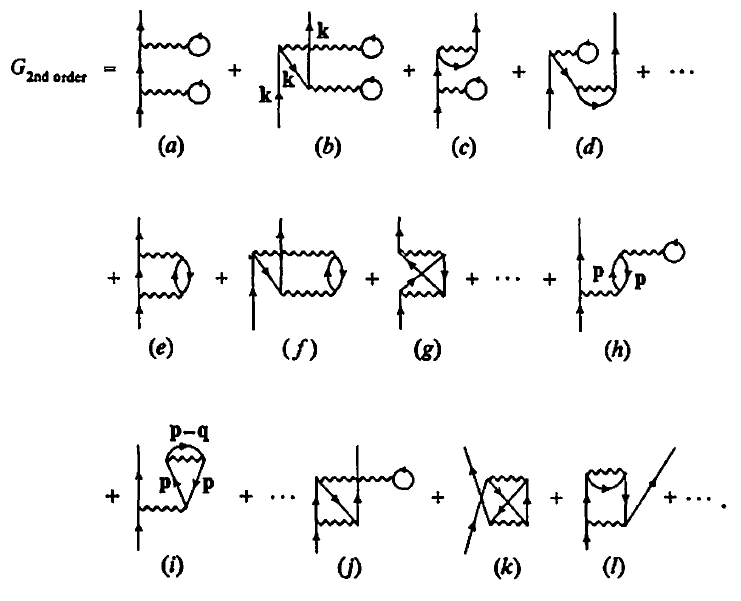
\includegraphics[width=0.8\textwidth]{screenshots/typical-2nd-order-diagrams.PNG}
    \label{typical-2nd-order-diagrams}
\end{equation}
\begin{equation}
    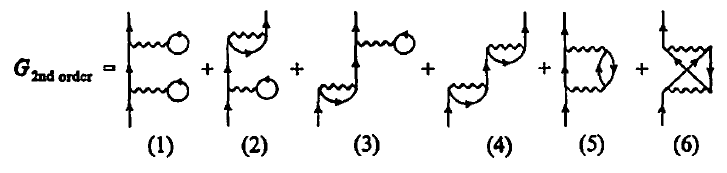
\includegraphics[width=0.8\textwidth]{screenshots/typical-2nd-order-diagrams-2.PNG}
    \label{typical-2nd-order-diagrams-2}
\end{equation}
\begin{equation}
    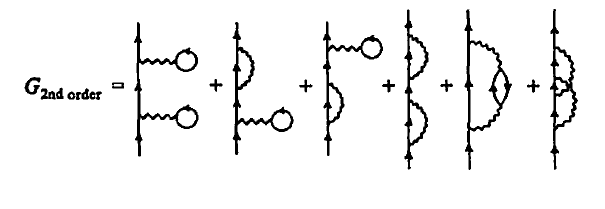
\includegraphics[width=0.8\textwidth]{screenshots/typical-2nd-order-diagrams-3.PNG}
    \label{typical-2nd-order-diagrams-3}
\end{equation}
Let us evaluate a typical second-order diagram using the Feynman method.
\begin{equation}
    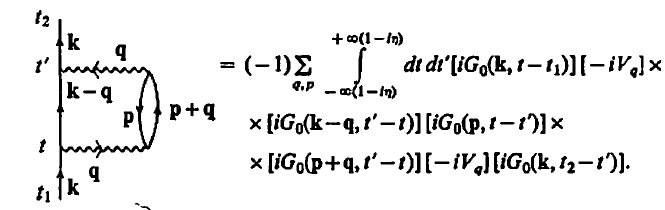
\includegraphics[width=0.8\textwidth]{screenshots/typical-feynman-diagrams-to-integral.PNG}
    \label{typical-feynman-diagrams-to-integral}
\end{equation}
Note that \redp{the order of the times in G is always: time at end of directed line minus time at beginning.} The Fourier transform of (\ref{typical-feynman-diagrams-to-integral}) is
\begin{equation}
    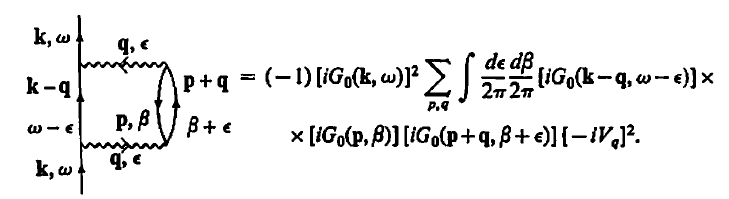
\includegraphics[width=0.8\textwidth]{screenshots/typical-feynman-diagrams-to-integral-fourier.PNG}
\end{equation}
It is seen that the frequencies, $\omega, \epsilon, \beta,$ etc., are conserved at the vertices, just like the momentum. This comes about because of the appearance of $\delta$ -functions similar to the $2 \pi \delta\left(\omega^{\prime}-\omega\right)$ when the transform is carried out. \bluep{\textbf{The "$2\pi$" in $\frac{d\epsilon}{2\pi}$ comes from Fourier transformation too.}}

One more thing, We can avoid treating the 'non-propagating' lines as a special case by including a convergence factor $exp(i\omega 0^+)$ when translating these lines into functions, where $0^+$ is a positive infinitesimal such that $0^{+} \times \infty=\infty$, thus
\begin{imp}
\begin{equation}
    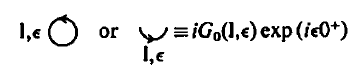
\includegraphics[width=0.8\textwidth]{screenshots/non-propagating-treatment.PNG}
\end{equation}
Hence the integral over the intermediate frequency $\epsilon$ gives:
\begin{equation}
\int_{-\infty}^{+\infty} \frac{d \epsilon}{2 \pi} \frac{i e^{i \epsilon 0^+}}{\epsilon-\epsilon_{l}+i \delta_l}=\begin{aligned}
-1 & \text { for } \quad l<k_{F} \\
0 & \text { for } \quad l>k_{F}
\end{aligned}\end{equation}
where $\delta_l=-\delta$ when $l<k_F$. The integral is done by contour residues theorem. The contour is closed in the upper half-complex-plane where the convergence factor makes the arc integral vanish.
\end{imp}
Thus, for example
$$
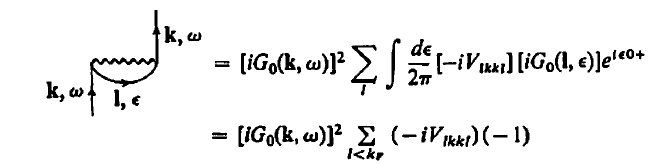
\includegraphics[width=0.8\textwidth]{screenshots/non-propagating-treatment-example.PNG}
$$

\subsection{Diagram rules for single-particle propagator}
We have now reached the point where we can present in summary form the rules for drawing and evaluating the type of graphs which will be used in the next two chapters. These are the diagrams describing a system of mutually interacting fermions with no external field and they will always be drawn in $(\mathbf{k},\omega)$-space, using the Feynman method. The rules are:

\begin{easylist}
\NewList
@ In nth order, drawn wiggly lines with vertex dots and two external points

@ Join all vertex dots and external points to each other with directed lines in all linked topologically distinct (in the Feynman sense) ways, with one line entering and one leaving each vertex dot and a line entering one external point and leaving the other. Two diagrams are topologically distinct if they are visualized as made of rubber bands, and one cannot be deformed into the other.

@ Label each line and wiggle with a momentum, k (short for $\mathbf{k}, \sigma,$ where $\boldsymbol{\sigma}=\operatorname{spin}),$ and frequency $\omega,$ such that the sum of momenta (and frequencies) entering each vertex = sum of those leaving. Eliminate all 'anomalous' or 'momentum-non-conserving' diagrams, i.e., which have a hole and a particle in the same state.

@ Evaluate graphs by means of the dictionary in the following table
\end{easylist}
\begin{table}[H]
    \centering
    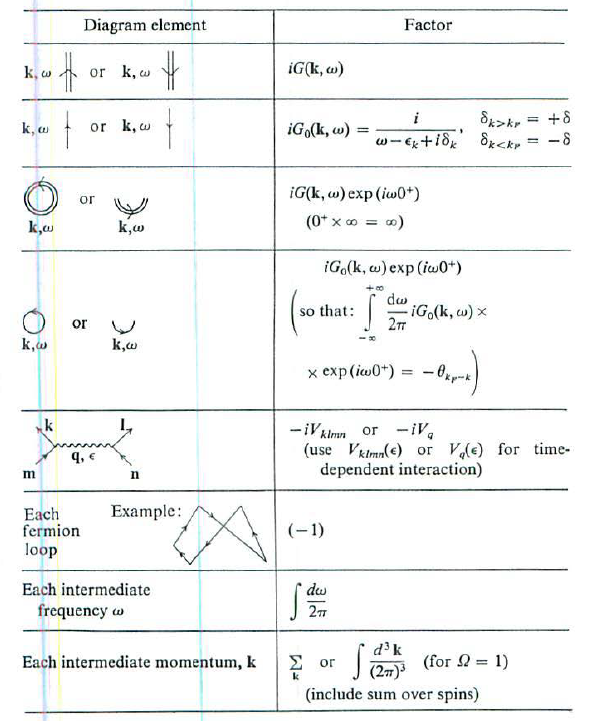
\includegraphics[width=0.6\textwidth]{screenshots/table-feynman-diagram-rules.PNG}
    \caption{Diagram dictionary for interacting many-fermion system with
no external potential (Feynman method)}
    \label{tab:feynman-diagram-rules}
\end{table}
Some physicists use abbreviated diagram in which the interaction wiggles are compressed to points or little squares. Thus, for example
\begin{equation}
    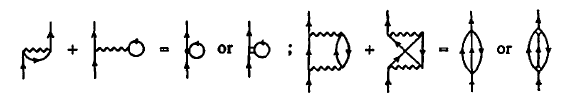
\includegraphics[width=0.8\textwidth]{screenshots/Hugenholtz-diagrams.PNG}
\end{equation}
Those drawn with points are called "Hugenholtz diagrams", while those with squares are "Abrikosov diagrams".

\subsection{Modified propagator formallsm using chemical potential,\texorpdfstring{$\mu$}{TEXT}}
The formalism just described can be somewhat inconvenient in actual calculations because, unless special precautions are taken, it may produce approximations for $G$ which yield the wrong total number of particles for the system.

In order to understand this, let us first derive the relation between the propagator $G$ and the total particle number N. The quantity N is the expectation value of the total number  operator $2\sum_k c^{\dagger}_k c_k$(factor of 2 for spin) in the interacting ground state:
\begin{equation}N=\left\langle\Psi_{0}\left|2 \sum_{k} c^{\dagger}_{k} c_{k}\right| \Psi_{0}\right\rangle=2 \sum_{k}\left\langle\Psi_{0}\left|c^{\dagger}_{k} c_{k}\right| \Psi_{0}\right\rangle\end{equation}
The summand is easily expressed in terms of $G(k_2,k_1,t_2-t_1)$ by setting $t_2=t,t_1=0,k_1=k_2=k$, then letting t approach zero from the left. This yields
\begin{equation}N=2 \sum_{k}(-i) \times \lim _{t \rightarrow 0^{-}} G(k, t)=-2 i \lim _{t \rightarrow 0^{-}} \int \frac{d^{3} \mathbf{k}}{(2 \pi)^{3}} \int \frac{d \omega}{2 \pi} G(\mathbf{k}, \omega) e^{-i \omega t}
\label{N-G-relation}
\end{equation}
which is the desired relation.

Imagine that we calculate an approximate G for the system by a partial summation over some types of diagrams in 
\begin{equation}
    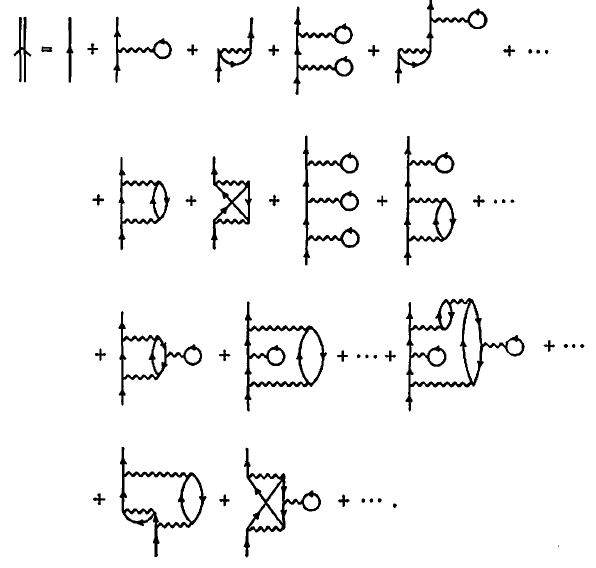
\includegraphics[width=0.8\textwidth]{screenshots/single-propagator-feynman-method.PNG}
    \label{single-propagator-feynman-method}
\end{equation}
and then place this G in (\ref{N-G-relation}) to check and see if it yields $N=N_0$. Evidently, $G$ will be a function of $N_0$, because each $G_0$ entering the calculation of $G$(approx.) depends on $k_F$, and $k_F$ is related to $N_0$ by
\begin{equation}N_{0}=2 \sum_{k<k_{P}} 1=\frac{2}{(2 \pi)^{3}} \int_{k<k=} d^{3} \mathbf{k}=k_{F}^{3} / 3 \pi^{2}, \quad \text { or } \quad k_{F}=\left(3 \pi^{2} N_{0}\right)^{1/3}\end{equation}
Note that the Fermi energy is
\begin{equation}c_{F}=k_{F}^{2} / 2 m=\frac{\left(3 \pi^{2} N_{0}\right)^{2/3}}{2 m}\end{equation}
\bluep{Hence N will be function of $N_0$. But, since $G$ is only approximate, there is no guarantee that $N$ will equal $N_0$}.

It is simple to remove this difficulty by slightly modify the formalism. The method of doing this is to \redp{use the "grand canonical ensemble" at zero temperature. In this method we no longer regard the system as isolated, with definite particle number $N_0$, but instead put it in contact with a particle reservior, so that it can gain or lose particles. Thus, particle number, N is variable throughout the calculation.} The chemical potential of system, $\mu$ is fixed but unknown; its value is determined at the end of the calculation by setting the total particle number equal to $N_0$.
\begin{imp}
The modified Hamiltonian for this case is
\begin{equation}H^{\prime}=H-\mu N=H_{0}^{\prime}+H_{1}\end{equation}
where
\begin{equation}\begin{aligned}
&H_{0}^{\prime}=\sum_{k}\left(\epsilon_{k}-\mu\right) c_{k}^{\dagger} c_{k}\\
&H_{1}=\frac{1}{2} \sum_{k l m n} V_{k l m n} c_{l}^{\dagger} c_{k}^{\dagger} c_{m} c_{n}
\end{aligned}\end{equation}
where N is the total particle number operator.
\end{imp}
The ground state of the modified unperturbed Hamiltonian, $H^{\prime}_{0},$ is obtained by selecting that number of particles, and that way of filling the energy levels which minimizes the energy. \textbf{\redp{It is easily seen that this means all levels filled up to $\epsilon_{k}=\mu, \text { i.e., up to } k_{F}^{\mu}=\sqrt{( 2 m \mu)}$}} The corresponding particle number is $N=\left(3 \pi^{2}\right)^{-1} \times(2 m \mu)^{3/2} .$ The free propagator for $H_{0}^{\prime}$ is
\begin{equation}G_{0}^{\mu}(\mathbf{k}, \omega)=\frac{1}{\omega-\left(\epsilon_{k}-\mu\right)+i \delta_{k}^{\mu}}, \quad \delta_{k}^{\mu}=\left\{\begin{array}{ll}
+\delta & \text { for } \epsilon_{k}>\mu \\
-\delta & \text { for } \epsilon_{k}<\mu
\end{array}\right.\end{equation}
It will be convenient to define a new $\omega$ such that $\omega_{\text {new }} \equiv \omega+\mu .$ In addition, in order to get the correct result when we do self-consistent Hartrec-Fock, it is necessary to re-write the infinitesimal in the form $i \operatorname{sign}(\omega-\mu) \delta$ or $i(\omega-\mu) \delta$ for short, where $\omega \equiv \omega_{\text {new }} .$ These two changes yield $\left(\omega \equiv \omega_{\text {new }}\right)$
\begin{equation}G_{0}^{\mu}(\mathbf{k}, \omega)=\frac{1}{\omega-\epsilon_{k}+i(\omega-\mu) \delta}
\label{G-0-mu}
\end{equation}
Now $N$ becomes a function of $\mu$. If $\mu$ is now determined by setting
\begin{equation}
N(\mu)=N_0
\label{N=N-0}
\end{equation}
we guarantee that $G$(approx.) yields the correct number of particles. Using (\ref{N-G-relation}), (\ref{G-0-mu}), and (\ref{N=N-0}), and ignoring interactions we have:
\begin{equation}N(\mu)=\frac{\left(k_{P}^{\mu}\right)^{3}}{(3 \pi)^{2}}=\frac{(2 m \mu)^{3/2}}{3 \pi^{2}}=N_{0}
\label{N0-kF-relation}
\end{equation}
so that $\mu=\epsilon_F$.
\newpage
\appendix
\section{Mismatch in subscript sequence}
In chapter 7 we have shown that the "two-body" interaction in occupation number formalism is:
\begin{equation}\mathcal{O}^{\mathrm{occ}}=\frac{1}{2} \sum_{k l m n} \mathcal{O}_{k l m n} c_{l}^{\dagger} c_{k}^{\dagger} c_{m} c_{n}\end{equation}
where
\begin{equation}\mathcal{O}_{k l m n}=\int d^{3} \mathbf{r} \int d^{3} \mathbf{r}^{\prime} \phi_{k}^{*}(\mathbf{r}) \phi_{l}^{*}\left(\mathbf{r}^{\prime}\right) \mathcal{O}\left(\mathbf{r}, \mathbf{r}^{\prime} ; \mathbf{p}, \mathbf{p}^{\prime}\right) \phi_{m}(\mathbf{r}) \phi_{n}\left(\mathbf{r}^{\prime}\right)\end{equation}
This appendix is dedicated to deal with the mismatch between the subscript of $O_{klmn}$ and that of $c^{\dagger}_lc^{\dagger}_kc_mc_n$.

Using the Dirac notation, we have, for a state in the occupation number formalism: 
\begin{equation}\left\langle n_{1}, n_{2}, \ldots, n_{i} \ldots|=| \overline{\left.n_{1}, n_{2}, \ldots, n_{i}\right\rangle}\right.\end{equation}
where the overline means the Hermitian adjoint. However, for a product of operators we have
\begin{equation}\left(\hat{\phi}_{k} \hat{\phi}_{l}\right)^{\dagger}=\hat{\phi}_{l}^{\dagger} \hat{\phi}_{k}^{\dagger}\end{equation}
Thus, for a two-body interaction $\hat{V}$ we have:
\begin{equation}\begin{aligned}
\hat{V} &=\frac{1}{2} \sum_{k l m n}\langle k, l|V| m, n\rangle=\frac{1}{2} \sum_{k l m n} \iint d \mathbf{r} d \mathbf{r}^{\prime}\left(\hat{\phi}_{k} \hat{\phi}_{l}\right)^{\dagger} V\left(\mathbf{r}-\mathbf{r}^{\prime}\right) \hat{\phi}_{m} \hat{\phi}_{n} \\
&=\frac{1}{2} \sum_{k l m n} \iint d \mathbf{r} d \mathbf{r}^{\prime} \hat{\phi}_{l}^{\dagger} \hat{\phi}_{k}^{\dagger} V\left(\mathbf{r}-\mathbf{r}^{\prime}\right) \hat{\phi}_{m} \hat{\phi}_{n}=\frac{1}{2} \sum_{k l m n} V_{k l m n} c_{l}^{\dagger} c_{k}^{\dagger} c_{m} c_{n}
\end{aligned}\end{equation}
where 
\begin{equation}V_{k l m n}=\iint d \mathbf{r} d \mathbf{r}^{\prime} \phi_{k}^{\dagger} \phi_{l}^{\dagger} V\left(\mathbf{r}-\mathbf{r}^{\prime}\right) \phi_{m} \phi_{n}\end{equation}
Thus we \textbf{don't have mismatches in Dirac notation to keep things intuitive, but we do need to take care of the effects of " † " when we translate the notation into integrals.}
\end{document}